
\chapter{Analisi}

Lo scopo di questo capitolo è quello di fornire un'analisi del sistema da proporre. Verrà specificato il contesto nel quale l'artefatto dovrà operare, mettendo in evidenzia l'insieme dei requisiti che dovranno risultare soddisfatti. 
%Per la struttura di questo capitolo verranno utilizzate le specifiche suggerite in \cite{ieee830-1998} come riferimenti.

\section{Scopo del sistema}

Il progetto \emph{MyCLIPS} si prefigge lo scopo di sviluppare un software di tipo \emph{Expert System Environment}, mediante la realizzazione di un ambiente multi-paradigmatico che unisca al classico modello dichiarativo basato su regole, meccanismi di  supporto alla programmazione procedurale.


% e basata su regole, un regime di controllo di tipo \emph{forward chaining} e un'implementazione dell'algoritmo RETE per le operazione di \emph{pattern-matching}.
Affiancato al sistema principale, verrà inoltre progettato un modulo aggiuntivo che consenta la distribuzione dei servizi offerti dal software principale tramite un modello d'architettura \emph{client-server}.

L'artefatto derivante dal progetto, inteso come unione del software principale e del modulo server aggiuntivo, non sarà un prodotto con fini commerciali, ma piuttosto uno strumento con finalità didattiche, di supporto alla ricerca nell'ambito degli \emph{environment per sistemi esperti} e all'integrazione degli stessi con tecnologie orientate al Web.

Nel campo degli \emph{environment}, il software CLIPS rappresenta un punto di riferimento sia nell'ambito dell'efficienza, che del numero di funzionalità offerte. La gratuità e la facile reperibilità del sistema ha garantito una larga adozione in ambito accademico. Il confronto fra il sistema proposto nell'ambito di questo progetto e il software CLIPS rappresenta una metrica per la valutazione del prototipo stesso. Un buon grado di compatibilità fra i due sistemi consentirebbe l'accesso ad un grande bacino di artefatti già prodotti per il sistema CLIPS.

%%%%% ATTIVARE PER COMPILAZIONE RAPPORTO-TECNICO %%%%%
% Include:
% 	- Sezione: Definizioni, acronimi, abbreviazioni
%\section{Definizioni, acronimi, abbreviazioni}

\begin{itemize}
	\item \emph{Ambiente di sviluppo integrato}:
	\item \emph{Analisi dei requisiti}:
	\item \emph{API}:
	\item \emph{Best Practice}:
	\item \emph{Bug}:
	\item \emph{C}:	
	\item \emph{Client}:
	\item \emph{Casi d'uso}:
	\item \emph{Codice sorgente}:
	\item \emph{CPU}:
	\item \emph{Design Pattern}:
	\item \emph{Eclipse}:
	\item \emph{Expert System Environment}:
	\item \emph{Forward Chaining}:
	\item \emph{GUI}:
	\item \emph{IDE}:
	\item \emph{Incapsulamento}:
	\item \emph{Incrementale}:
	\item \emph{Java}:
	\item \emph{Javadoc}:
	\item \emph{Listener}:
	\item \emph{Multipiattaforma}:
	\item \emph{MyCLIPS}:
	\item \emph{Multi-slot}:
	\item \emph{Open source}:
	\item \emph{Overhead}:
	\item \emph{Package}:
	\item \emph{Pattern Matching}:
	\item \emph{Plugin}:
	\item \emph{PyDev}:
	\item \emph{Python}:
	\item \emph{RETE}:
	\item \emph{Slot}:
	\item \emph{Strategia di risoluzione dei conflitti}:
	\item \emph{Rule-Based Systems}:
	\item \emph{Server}:
	\item \emph{Sistema Operativo}:
	\item \emph{Skeleton}:
	\item \emph{Standalone}:
	\item \emph{Stub}:
	\item \emph{Thread}:
	\item \emph{UML}:
	\item \emph{Unificazione}:
	\item \emph{Use Case}:
	\item \emph{XML}:
	\item \emph{XMLRPC}:
\end{itemize}


%%%%% ATTIVARE PER COMPILAZIONE RAPPORTO-TECNICO %%%%%
% Include:
% 	- Sezione: Riferimenti
%\include{Rapp-tecnico/riferimenti}

\section{Capacità}

Il tipo di software che il progetto MyCLIPS punta a realizzare è un \emph{environment} multi-paradigmatico per sistemi esperti. In quanto tale deve offrire strumenti per la realizzazione di sistemi esperti, associando all'uso delle regole di produzione come metodo di rappresentazione della conoscenza, la possibilità di specifica di strutture di controllo tramite un paradigma procedurale.


Si riassumono schematicamente le funzionalità principali richieste al sistema, offrendo anche un riferimento al paragrafo nel quale la capacità viene approfondita e analizzata nel dettaglio:

\begin{enumerate}
	\item l'uso di un linguaggio di specifica che consenta:
		\begin{enumerate}
			\item la definizione di regole di produzione (\ref{par:linguaggio-regole})
			\item l'utilizzo di un paradigma procedurale (\ref{par:linguaggio-funzioni})
			\item la specifica di funzioni utente (\ref{par:linguaggio-funzioni})
			\item la specifica di moduli (\ref{par:linguaggio-moduli})
			\item definizione di template di fatti (\ref{par:linguaggio-template})
			\item la specifica della conoscenza fattuale tramite:
				\begin{enumerate}
					\item fatti in notazione Ordered-Fact (\ref{par:linguaggio-fatti})
					\item fatti in notazione Template-Fact (\ref{par:linguaggio-fatti})
				\end{enumerate}
		\end{enumerate}
	\item la possibilità di aggiungere strategie di risoluzione dei conflitti (\ref{par:strategie-crs})
	\item la possibilità di integrare nuove funzioni di sistema (\ref{par:motore-inferenziale})
	\item compatibilità con i sistemi sviluppati per CLIPS:
		\begin{enumerate}
			\item compatibilità del linguaggio di specifica (\ref{par:linguaggio})
			\item compatibilità delle strategie di risoluzione dei conflitti (\ref{par:strategie-crs})
			\item compatibilità con un \emph{sub-set} delle funzioni di sistema
		\end{enumerate}
	\item l'utilizzo dell'algoritmo RETE per le operazioni di \emph{Pattern-Matching}~(\ref{par:algoritmo-rete})
	\item la possibilità di accedere alle funzionalità del sistema tramite un terminale~(\ref{par:terminale})
	\item la distribuzione delle funzionalità del software tramite un modulo server~(\ref{par:server})
\end{enumerate}


\subsection{Linguaggio di specifica}\label{par:linguaggio}

La compatibilità fra l'\emph{environment} prodotto e il sistema CLIPS rappresenta una delle capacità desiderate. Per realizzarla è necessario consentire l'utilizzo degli artefatti precedentemente prodotti utilizzando il linguaggio di specifica fornito da CLIPS. La restrizione delle capacità richieste alla sola fornitura delle meccaniche di definizione delle regole di produzione e delle strutture di controllo procedurali, consente di restringere l'insieme dei costrutti che è necessario definire escludendo i formalismi di specifica relativi al paradigma di sviluppo orientato agli oggetti concentrati nel sotto-sistema COOL di CLIPS.

%Fra le capacità del sistema è richiesta la fornitura di un linguaggio di specifica che permetta l'utilizzo di sistemi esperti realizzati per il software CLIPS. Il livello di compatibilità previsto richiede di fornire all'utente i costrutti di base utilizzati da CLIPS per la definizione di regole, della conoscenza fattuale (in formato \emph{Ordered-Fact} e \emph{Template-Fact}), dei moduli, delle funzioni utente e delle variabili globali.

Il linguaggio utilizzato deve risultare compatibile sia a livello semantico che a livello sintattico con quello fornito da CLIPS, offrendo in questo modo il massimo livello di portabilità degli artefatti.

\subsubsection{Moduli}\label{par:linguaggio-moduli}
Il formalismo previsto da CLIPS e che dovrà essere supportato dal software prodotto, consente la definizione di moduli attraverso l'utilizzo del costrutto \emph{defmodule}.
Il modulo è un'unità di programma che racchiude e organizza la definizione di ulteriori costrutti. Lo scambio delle definizioni fra moduli differenti è previsto attraverso un protocollo di \emph{import/export}.

\begin{program}
\verbatimtabinput[3]{Capitoli/capitolo-2/bnf/defmodule.txt}
\caption{Specifica \emph{BNF} del costrutto \emph{defmodule}}
\end{program}

La sintassi prevede di associare un nome univoco ad ogni modulo, oltre alla possibilità di specificare un elenco di costrutti da rendere disponibili all'esterno del modulo stesso (tramite l'attributo \emph{export}), oppure un elenco di definizioni da importare da un modulo precedentemente creato (tramite l'attributo \emph{import}).


\subsubsection{Funzioni utente}\label{par:linguaggio-funzioni}
All'utente, in maniera alternativa all'integrazione di funzioni scritte in linguaggio nativo, deve essere offerta la possibilità di aggiungere funzioni personalizzate all'interno del sistema utilizzando il costrutto \emph{deffunction} (Codice~\ref{code:deffunction}). La definizione di funzioni consente di specificare strutture di controllo procedurali che eseguano sequenze di operazioni guidate dai parametri di chiamata.

\begin{program}
\verbatimtabinput[3]{Capitoli/capitolo-2/bnf/deffunction.txt}
\caption{Specifica \emph{BNF} del costrutto \emph{deffunction}}\label{code:deffunction}
\end{program}


Le funzioni cosi integrate potranno essere utilizzate nelle stesse modalità previste dalle altre funzioni di sistema, con l'eccezione relativa ai vincoli di visibilità fra moduli.

\begin{program}
\begin{verbatimtab}

(defmodule A
	(export deffunction Funzione_Di_Prova))
	
(deffunction A::Funzione_Di_Prova () )

(defmodule B
	(import A deffunction Funzione_Di_Prova))
\end{verbatimtab}
\caption{Esempio di scambio di una definizione fra moduli}\label{code:deffunction-import}
\end{program}

Le definizioni di funzioni devono essere esportate dal modulo in cui sono definite e successivamente importate da quello che intende utilizzarle (Codice~\ref{code:deffunction-import}).

\subsubsection{Regole}\label{par:linguaggio-regole}
La specifica di regole deve essere resa disponibile tramite l'utilizzo del costrutto \emph{defrule}~(Codice~\ref{code:defrule}).

\begin{program}
\verbatimtabinput[3]{Capitoli/capitolo-2/bnf/defrule.txt}
\caption{Specifica \emph{BNF} del costrutto \emph{defrule}}\label{code:defrule}
\end{program}

La porzione \emph{LHS} e \emph{RHS} della regola sono separati dal simbolo $=>$. I \emph{pattern} della \emph{LHS} sono definiti con riferimento ai formalismi utilizzati per la specifica di \emph{Ordered-Fact} e \emph{Template-Fact}. Le variabili vengono specificate attraverso l'uso di \emph{wildcard}, identificate dalla presenza del simbolo ''?'' come primo carattere. I \emph{pattern} possono essere ulteriormente specificati tramite l'utilizzo di connettivi logici come \emph{not}, \emph{or} e \emph{and}, oppure espressioni logiche come \emph{exists} o \emph{test}.
La porzione \emph{RHS} contiene chiamate a procedure di sistema o definite dall'utente tramite il costrutto \emph{deffunction}.


\subsubsection{Fatti}\label{par:linguaggio-fatti}

I \emph{fatti} costituiscono il contenuto della \emph{working memory}. Il linguaggio fornito deve prevedere, parallelamente a quanto previsto da CLIPS, la definizione dei fatti attraverso la notazione \emph{Ordered-Fact} e \emph{Template-Fact}.

\begin{program}
\verbatimtabinput[3]{Capitoli/capitolo-2/bnf/deffacts.txt}
\caption{Specifica \emph{BNF} del costrutto \emph{deffacts}}\label{code:deffacts}
\end{program}


La specifica dei fatti deve essere riunita all'interno di costrutti \emph{deffacts}~(Codice~\ref{code:deffacts}). Questo consente di inserire un elenco di definizioni che verranno automaticamente asserite durante la fase di inizializzazione del sistema esperto.

Il primo formato di specifica dei fatti, chiamato \emph{Ordered-Fact}, prevede la definizione degli stessi come vettori di elementi simbolici o numerici di lunghezza arbitraria. Il formato del primo elemento è richiesto che sia di tipo \emph{SYMBOL}\footnote{SYMBOL rappresenta un tipo elementare presente in CLIPS. Appartengono a questo tipo tutte le sequenze alfanumeriche non delimitate da apici e che abbiano come primo elemento un carattere alfabetico}, il formato dei successivi elementi è arbitrario.

La seconda modalità di specifica, denominata \emph{Template-Fact}, prevede la definizione dei fatti tramite l'utilizzo di un \emph{template} e una sequenza di \emph{slot}. Gli slot rappresentano delle caratteristiche definite nella specifica del \emph{template}.
La definizione del fatto può prevedere l'avvaloramento di tutti o solo una porzione degli \emph{slot} previsti dal \emph{template}.
I valori inseribili negli \emph{slot} possono essere singoli elementi o multipli. Nel secondo caso si farà riferimento allo \emph{slot} con il nome di \emph{multi-slot}.

\subsubsection{Template}\label{par:linguaggio-template}

La specifica dei fatti in formato \emph{Template-Fact} prevede la definizione preventiva di un \emph{template} che definisca una ''tipologia'' di fatti, indicata con un nome univoco e una sequenza di caratteristiche: \emph{slot} e \emph{multi-slot}~(Codice~\ref{code:deftemplate}).

\begin{program}
\verbatimtabinput[3]{Capitoli/capitolo-2/bnf/deftemplate.txt}
\caption{Specifica \emph{BNF} del costrutto  \emph{deftemplate}}\label{code:deftemplate}
\end{program}

La specifica prevede la definizione di valori di \emph{default}, da attribuire nei casi in cui non venga fornito un valore durante l'asserzione, oppure di restrizioni sul tipo di valori utilizzabili nello \emph{slot}.

\subsection{Parser}\label{par:parser}

Le funzionalità di analisi ed interpretazione dei costrutti specificati tramite il linguaggio di definizione sono racchiuse all'interno del \emph{parser}. Utilizzando una serie di regole sintattiche, questo componente è in grado di leggere le definizioni dei costrutti previsti dal linguaggio e convertirle in elementi computabili dal motore inferenziale.

Ad ogni costrutto definito dal linguaggio vengono associate una serie di regole sintattiche che descrivono i vincoli di validità e come convertire le varie definizioni, una volta individuate. Le regole vengono specificate attraverso l'alternanza di sequenze simboliche predefinite e campi variabili, che rappresentano le proprietà dei singoli costrutti.

Le regole vengono organizzate in strutture nidificate. Il riconoscimento di determinate sequenze simboliche relative ad una regola principale, spesso delimitate da parole chiave, attiva la possibilità di utilizzare sotto-regole associate a quella principale.

Il linguaggio di definizione prevede la possibilità di definire elementi in grado di alterare le regole sintattiche utilizzate dal \emph{parser}, come \emph{template} o \emph{funzioni}. Questo comporta la necessità di strutturare il processo di conversione come un'alternanza di fasi di analisi ed interpretazione, eseguite su singoli costrutti individualmente.

\subsection{Motore inferenziale}\label{par:motore-inferenziale}

Il motore inferenziale controlla il processo di ragionamento alla base di un sistema esperto. Il ragionamento è strutturato attraverso meccanismi di inferenza, che in questo sistema vengono esplicitati nella forma di regole di produzione.

L'utilizzo del motore inferenziale è regolato da quattro fasi:

\begin{enumerate}
	\item \emph{l'inizializzazione}, caricando conoscenza procedurale e fattuale. Il caricamento avviene attraverso la definizione di regole e gruppi di fatti iniziali. Le modalità con le quali gli elementi vengono specificati possono essere legate all'utilizzo del linguaggio di definizione o alla specifica diretta dei costrutti in una forma direttamente utilizzabile dal motore inferenziale. Nel primo caso sarà necessaria una fase di conversione delle definizioni, onere del parser.
	\item la \emph{preparazione}, nella quale il motore inferenziale organizza gli elementi ottenuti nella fase precedente all'interno di strutture specifiche che agevolino le elaborazioni successive. 
	%In questa fase l'insieme di regole viene trasformato nelle strutture utilizzate dall'algoritmo RETE per le operazioni di pattern-matching.
	\item l'\emph{esecuzione}, nella quale viene eseguito il ciclo \emph{recognize-act}.
	\item la \emph{valutazione}, una fase nella quale può essere analizzato lo stato finale nel quale ha avuto termine l'elaborazione.
\end{enumerate}

%Le fasi di preparazione ed esecuzione previste dal motore inferenziale garantiscono un utilizzo dello stesso
La realizzazione del ciclo di controllo \emph{recognize-act} prevede il confronto fra le condizioni espresse nelle porzioni \emph{LHS} delle regole e l'insieme di fatti memorizzato all'interno della memoria di lavoro. La verifica dell'applicabilità delle regole deve essere ripetuta come conseguenza di ogni modifica, anche minima, della memoria di lavoro. Per ridurre lo sforzo elaborativo richiesto dalle operazioni di confronto è possibile utilizzare l'algoritmo RETE~\cite{forgy1979}~\cite{forgy1982}~\cite{Doorenbos95productionmatching}.

\subsubsection{Algoritmo RETE}\label{par:algoritmo-rete}

\begin{figure}[h]
\centering
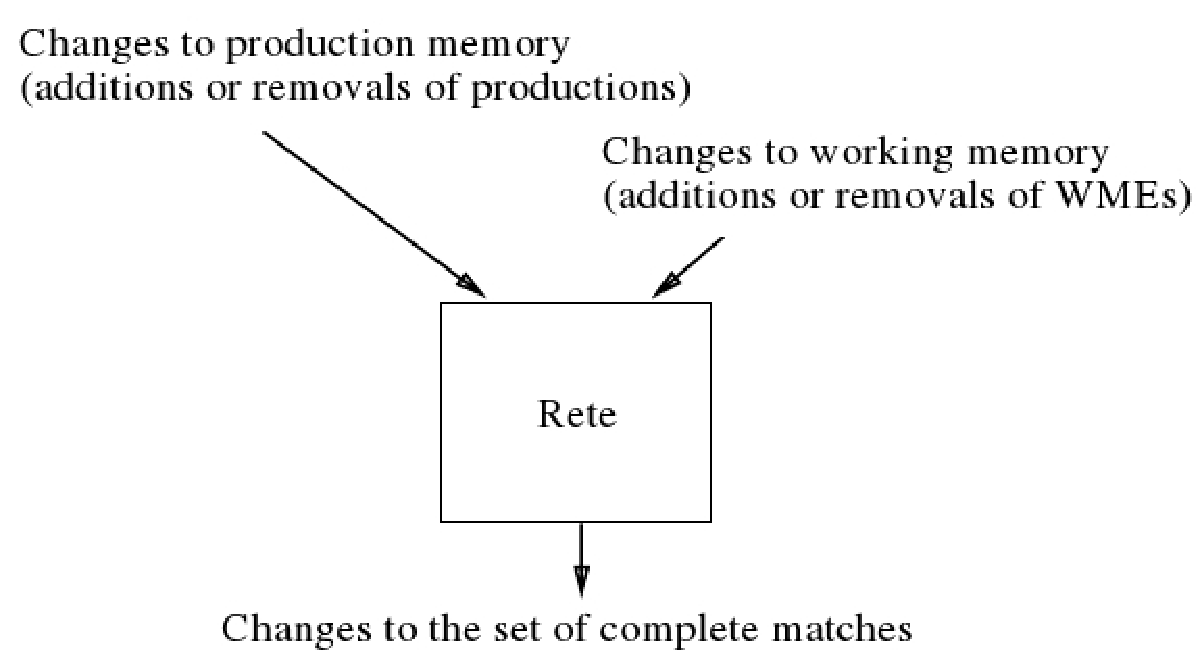
\includegraphics[scale=0.5, viewport=0 0 574 307]{Immagini/Capitolo2/Rete-blackbox.pdf}
\caption[RETE come una \emph{black-box}]{RETE come una \emph{black-box}: immagine originale tratta da \cite{Doorenbos95productionmatching}.}\label{fig:rete-black-box}
\end{figure}

L'algoritmo di \emph{pattern-matching} RETE consente un confronto efficiente fra il \emph{rules-set} e lo stato della \emph{working-memory}. Le attività svolte dall'algoritmo sono assimilabili a quelle di una \emph{black-box}~(\figurename~\ref{fig:rete-black-box}) alla quale vengono sottoposte due categorie di eventi: l'aggiunta o rimozione di regole e la modifica della \emph{working-memory}, intesa come asserzioni e ritrattazioni di fatti. Il risultato è in ogni caso un \emph{delta} delle attivazioni, un insieme di attivazioni da aggiungere o rimuovere dal \emph{conflict-set}~\cite{Doorenbos95productionmatching}.

Le attività legate alla modifica del \emph{rules-set} vengono normalmente svolte nelle fasi di preparazione del motore inferenziale, anche se questa assunzione non lede minimamente le possibilità di modifica del \emph{network} durante l'esecuzione. Le attività di valutazione delle modifiche alla \emph{working-memory} sono svolte sia nelle fasi di preparazione, valutando l'insieme di fatti iniziali, che di esecuzione, valutando asserzioni e ritrattazioni eseguite durante il ciclo \emph{recognize-act}.

\paragraph{Compilazione delle regole}

Il processo di \emph{compilazione} di una regola prevede la conversione dei \emph{pattern} presenti nella porzione \emph{LHS} delle regole in un grafo di valutazione. Ad ogni singolo \emph{pattern} deve essere fatto corrispondere un circuito che valuti le componenti statiche del pattern e che non richiedono un confronto con altri elementi della \emph{LHS}. Questo genere di confronti si definisce \emph{intra-element}. Le espressioni variabili vengono ignorate nell'esecuzione di questa classe di valutazioni.

I singoli circuiti vengono riuniti attraverso strutture che consentano di verificare la coerenza dei valori associati alle parti variabili, qualora queste ultime siano presenti in più di un \emph{pattern}. Questa classe di confronti viene definita \emph{inter-element}.

Il tipo di strutture che è possibile utilizzare durante il processo di conversione delle regole determina il tipo di confronti e operazioni che verranno effettuati durante fase di valutazione delle modifiche. Il processo di conversione può essere realizzato tramite la creazione di espressioni statiche, eseguite in sequenza per valutare le modifiche della \emph{working-memory}~\cite{forgy1979}~\cite{forgy1982} realizzando in questo modo una rappresentazione implicita di un grafo di valutazione. Questa forma di implementazione prende il nome di formulazione compilata. Una variante alternativa~\cite{Doorenbos95productionmatching} prevede la generazione esplicita del grafo attraverso la realizzazione di strutture che rappresentino i nodi, prendendo il nome di formulazione interpretata.

Il linguaggio di specifica~(Codice~\ref{code:defrule}) permette di esplicitare sia \emph{pattern} che verifichino l'esistenza diretta di fatti nella \emph{working-memory} (\texttt{Template\--Pattern\--CE}, \texttt{Ordered-Pattern-CE} e \texttt{Assigned-Pattern-CE}), che utilizzare connettivi logici per alterare il significato delle \emph{pattern}. I connettivi vengono esplicitati tramite \texttt{Not-CE} (negazione), \texttt{And-CE} (congiunzione), \texttt{Or-CE} (disgiunzione inclusiva). Queste condizioni possono essere valutate realizzando strutture apposite che eseguano i test tenendo conto del contesto offerto dal connettivo logico nel quale sono valutati. La formulazione proposta in \cite{Doorenbos95productionmatching} copre questi casi.
L'unica eccezione riguarda la disgiunzione inclusiva, la quale richiede invece una valutazione più approfondita per poter essere supportata dall'algoritmo.

\subparagraph{Compilazione di disgiunzioni inclusive}

La struttura della \emph{LHS} è implicitamente inclusa all'interno di un elemento condizionale \texttt{and} che verifichi la validità contemporanea di tutti i \emph{pattern}. La topologia dell'algoritmo RETE base~\cite{forgy1979}~\cite{forgy1982}~\cite{Doorenbos95productionmatching} però non consente la combinazione di elementi condizionali \texttt{and} e \texttt{or}. Per risolvere questo problema, garantendo l'utilizzo degli elementi \texttt{or-CE} nella specifica della \emph{LHS}, è possibile generare regole multiple per le quali sia garantita la conformità alla topologia di RETE da una singola regola contenente l'elemento \texttt{or}. 
L'operazione di compilazione deve essere preceduta da tre fasi: trasformazione, riduzione e scomposizione.

\begin{figure}[h]
\centering
\begin{minipage}[t]{5.5cm}
\begin{lstlisting}[numbers=none]
(and
	(or <CE1> <CE2>)
	(or <CE3> <CE4>))
\end{lstlisting}
\end{minipage}
\ \hspace{2mm} \hspace{3mm} \
\begin{minipage}[t]{5.5cm}
\begin{lstlisting}[numbers=none]
(or	
	(or
		(and <CE1> <CE3>)
		(and <CE1> <CE4>))
	(or
		(and <CE2> <CE3>)
		(and <CE2> <CE4>)))
\end{lstlisting}
\end{minipage}
\caption[Applicazione delle proprietà dei connettivi logici]{Applicazione delle proprietà dei connettivi logici per eseguire una normalizzazione dei \emph{pattern}. A sinistra la forma iniziale, a destra quella convertita}\label{fig:esempio-normalizzazione}
\end{figure}

La fase di trasformazione consiste nello sfruttare le proprietà dei connettivi logici per eseguire una conversione dei \emph{pattern} della \emph{LHS}~(\figurename~\ref{fig:esempio-normalizzazione}) fino ad ottenere una forma normalizzata che assicuri l'eventuale presenza di elementi \texttt{or} solo come elementi radice o contenuti in ulteriori \texttt{or}.

\begin{figure}[h]
\centering
\begin{minipage}[t]{5.5cm}
\begin{lstlisting}[numbers=none]
(or	
	(or
		(and <CE1> <CE3>)
		(and <CE1> <CE4>))
	(or
		(and <CE2> <CE3>)
		(and <CE2> <CE4>)))
\end{lstlisting}
\end{minipage}
\ \hspace{2mm} \hspace{3mm} \
\begin{minipage}[t]{5.5cm}
\begin{lstlisting}[numbers=none]
(or	
	(and <CE1> <CE3>)
	(and <CE1> <CE4>)
	(and <CE2> <CE3>)
	(and <CE2> <CE4>))
\end{lstlisting}
\end{minipage}
\caption[Riduzione dei connettivi \texttt{or} adiacenti]{Riduzione dei connettivi \texttt{or} adiacenti. A sinistra la forma iniziale, a destra quella ridotta}\label{fig:esempio-riduzione}
\end{figure}


La fase di riduzione consente di eliminare connettivi logici ridondanti, riducendo connettivi \texttt{or} e \texttt{and} adiacenti~(\figurename~\ref{fig:esempio-riduzione}).

Come ultima fase, quella della scomposizione, i singoli \texttt{and-CE} contenuti all'interno della clausola \texttt{or} vengono scomposti come fossero regole differenti. Ad ognuna di esse verrà associato la medesima porzione \emph{RHS}. Le regole scomposte verranno collegate alla regola principale e rimosse contemporaneamente come fossero una singola istanza.


\paragraph{Valutazione delle modifiche}

Durante la fase di esecuzione del ciclo \emph{recognize-act} ha invece luogo la seconda attività prevista dall'algoritmo RETE: la valutazione delle modifiche della \emph{working-memory}. L'aggiunta o la rimozione di elementi dalla memoria di lavoro viene valutata tramite l'\emph{attraversamento} del grafo di valutazione generato nella fase di preparazione. Gli elementi \emph{WME} verranno riuniti durante l'attraverso della regione \emph{beta} di valutazione all'interno di strutture complesse, i \emph{Token}.
Le attivazioni parziali di pattern singoli vengono memorizzati in memorie locali poste come terminali della regione \emph{alpha}, realizzando una frontiera.
Le attivazioni parziali di sequenze di pattern vengono riunite nei \emph{Token} e stoccate in memorie locali poste come conseguente della struttura che ha eseguito \emph{Join} fra i pattern.
L'output offerto dalla valutazione, ottenuto dai nodi terminali, consiste nell'elenco di attivazioni da aggiungere o rimuovere dall'agenda delle attivazioni.

\subsubsection{Risoluzione dei conflitti}\label{par:strategie-crs}

La selezione dell'attivazione da eseguire viene effettuata utilizzando una serie di criteri. L'entità che racchiude questi criteri e li organizza prende il nome di \emph{strategia di risoluzione dei conflitti} (CRS). La CRS organizza l'elenco di attivazioni disponibili per ogni stato del sistema in base ad un ordinamento specifico. L'aggiunta o la rimozione di un fatto può determinare l'aggiornamento dell'intera sequenza. Per ogni iterazione del ciclo \emph{recognize-act} possono essere aggiunte o rimosse un numero arbitrario di attivazioni determinate dalla modifica allo stato del sistema eseguita nella fase \emph{act}. All'inizio di ogni ciclo, l'attivazione con priorità maggiore (sempre determinata in base ai criteri della CRS in uso) viene selezionata, rimossa dalla sequenza e quindi eseguita.

Il software deve fornire diverse strategie di risoluzione di conflitti:
\begin{description}
	\item[Depth:] ad attivazioni più recenti viene associata una priorità maggiore.
	
	\item[Breadth:] le nuove attivazioni vengono inserite nella sequenza con priorità inferiore a quelle già esistenti.
	
	\item[Simplicity:] viene utilizzato come criterio per determinarne la priorità un indice di generalità della regola. A quelle con un minor grado di specializzazione verrà attribuita una priorità maggiore. Il coefficiente di complessità di ogni regola viene determinato prendendo in esame il numero di pattern presenti nella LHS, il numero di variabili utilizzate in ogni pattern ed il numero di connettivi ed espressioni logiche presenti. Il coefficiente, espresso tramite un valore numerico intero, viene quindi computato sommando le singoli componenti.
	
	\item[Complexity:] la specificità della regola a cui fa riferimento l'attivazione determina la priorità di attivazione. Il coefficiente di complessità viene calcolato in maniera analoga a quanto fatto per la CRS \emph{Simplicity}, ma valori di complessità maggiori determineranno una maggiore priorità.
	\item[Lex:] la priorità di attivazione viene calcolata come segue:
		\begin{itemize}
			\item ad ogni fatto viene attribuita un'etichetta temporale per determinare una relazione d'ordine.
			\item i fatti relativi ad ogni attivazione vengono quindi riordinati in modo decrescente.
			\item le attivazioni vengono confrontate prendendo in esame le sequenze ordinate di etichette temporali e assegnando priorità maggiore alle attivazioni con sequenze più recenti.
		\end{itemize}
	\item[Mea:] la priorità di attivazione viene calcolata come segue:
		\begin{itemize}
			\item ad ogni fatto componente l'attivazione viene attribuita un'etichetta temporale per determinare una relazione d'ordine fra i fatti nella \emph{working-memory}.
			\item per ogni attivazione viene identificata l'etichetta temporale più recente
			\item le etichette vengono confrontate assegnando priorità maggiore all'attivazione con etichetta più recente.
		\end{itemize}
	\item[Random:] le attivazioni vengono ordinate in modo casuale.
\end{description}

Un ulteriore criterio discriminante comune a tutte le CRS è quello basato sulla valutazione della \emph{salience}. Ad ogni regola può essere associato un valore numerico intero per determinare esplicitamente una relazione d'ordine. Qualora questo valore non venga indicato durante la definizione, ne verrà attribuito uno di \emph{default}. La valutazione della \emph{salience} è il primo elemento discriminante per il computo della priorità. Per le attivazioni relative a regole con la stessa \emph{salience} viene utilizzata la strategia di risoluzione dei conflitti per effettuare l'ordinamento.

In aggiunta alle CRS fornite con il software, deve essere fornita la possibilità di integrare ulteriori strategie di risoluzione di conflitti.

\subsection{Terminale}\label{par:terminale}

Il terminale è la forma di utilizzo del sistema più immediata prevista. Permette ad un utente di inizializzare il motore inferenziale ed eseguire elaborazioni, rendendo il software un'applicazione a sé. 

Alla base del funzionamento del terminale ci sono le funzionalità offerte dal parser. L'utilizzo del linguaggio di definizione permette di caricare o definire i sistemi esperti o, più genericamente, impartire una sequenza di comandi al software.

Un comando non è altro che una funzione di sistema oppure una funzione utente definita attraverso il costrutto \emph{deffunction}. La chiamata di una procedura viene eseguita fornendo un nome univoco che rimandi alla funzione, la quale può essere accompagnata da un insieme di parametri che ne specifichino i dati di ingresso. Il numero ed il tipo dei parametri che è possibile fornire è definito dalla \emph{firma} della funzione. Questa è una struttura che definisce la funzione stessa indicando un nome univoco, il numero ed il tipo di parametri ammissibili come dati d'ingresso e il tipo dell'output fornito dalla funzione.

\subsection{Modulo Server}\label{par:server}

Il software deve essere accompagnato da un componente in grado di rendere fruibili le funzionalità offerte attraverso un modello di architettura distribuita \emph{client-server}.

Un sistema distribuito consiste di una collezione di componenti, suddivisi su diversi terminali (anche chiamati \emph{host}) connessi fra loro attraverso un canale di comunicazione. Questi componenti interagiscono fra loro al fine di scambiare dati od accedere reciprocamente a servizi disponibili~\cite{Mascolo:2002:MCM:770420.770423}.
La realizzazione di un sistema distribuito è soggetta alla predisposizione di un sistema di comunicazione fra i processi collocati nei vari \emph{host}.

\begin{figure}[h]
\centering
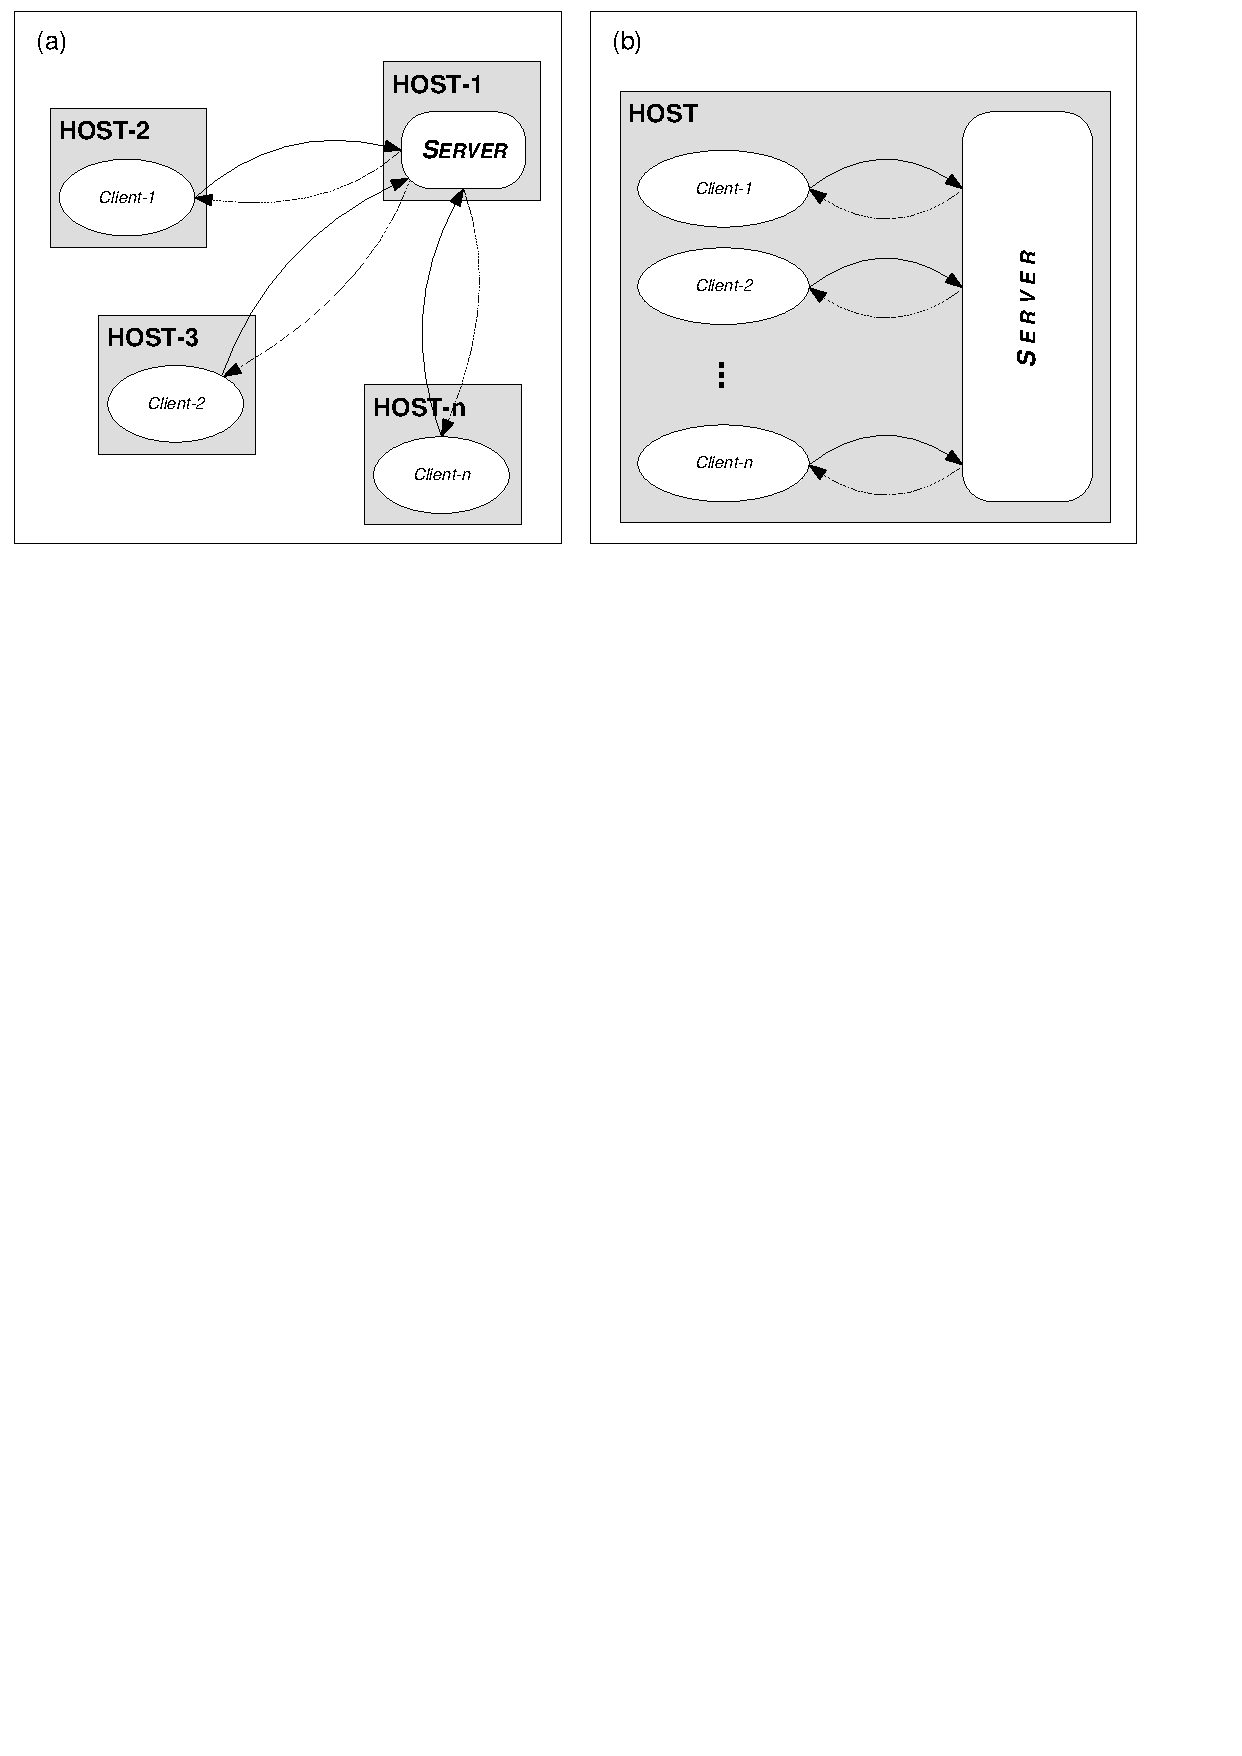
\includegraphics[scale=0.7, viewport=6 582 546 838]{Immagini/Capitolo2/Client-Server.pdf}
\caption[Architettura \emph{Client-Server}]{Architettura \emph{Client-Server}: in \emph{(a)} è mostrata una distribuzione su \emph{host} multipli, in \emph{(b)} una distribuzione in processi multipli}\label{fig:client-server}
\end{figure}

Il modello di architettura \emph{Client-Server} si basa sul partizionamento delle attività, risorse e responsabilità del sistema in due classi di componenti: \emph{Server} e \emph{Client}.
I componenti possono essere posizionati su \emph{host} fisicamente differenti, così come possono essere collocati in processi separati residenti sulla stessa macchina, in modo tale che non condividano direttamente risorse (\figurename~\ref{fig:client-server}). Lo scambio di informazioni avviene attraverso un protocollo noto ad entrambi i componenti.

Il modulo \emph{server} deve garantire la fruizione dei servizi offerti dall'\emph{en\-vi\-ron\-ment} a \emph{client} multipli contemporaneamente. \`E quindi necessario che i risultati intermedi di elaborazione, così le informazioni relative all'\emph{engine} e all'artefatto caricato, siano disponibili ed utilizzabili solo dal \emph{client} che ha eseguito il caricamento e le precedenti elaborazioni. Per supportare questo modello d'utilizzo, il \emph{server} deve essere in grado di associare un contesto univoco ad ogni richiesta che preveda l'utilizzo di risorse allocate in richieste precedenti.

L'inizializzazione del contesto deve essere richiesta dal \emph{client}: il \emph{server} provvederà all'allocazione delle risorse ed alla generazione di un identificativo di sessione univoco che verrà quindi fornito al \emph{client} e utilizzato dallo stesso per associare richieste successive al contesto inizializzato. Il server utilizza la sessione per memorizzare risultati parziali fra richieste successive, parametri di configurazione della comunicazione con il \emph{client} e, più genericamente, qualsiasi genere di informazione che possa essere ritenuta utile nel proseguo dell'elaborazione. Ogni sessione deve essere associata ad un tempo massimo di inattività oltre il quale la stessa venga rimossa automaticamente per consentire il recupero delle risorse allocate. Il tempo di inattività associato alla sessione deve essere calcolato tenendo presente l'ultima richiesta effettuata che abbia fornito l'identificativo come parametro di contesto. La rimozione della sessione può anche essere arbitrariamente richiesta dal \emph{client} che l'ha generata, nel momento in cui la stessa non sia ritenuta più necessaria.



%L'architettura \emph{Client-Server} descrive un modello di collaborazione fra sistemi. Il \emph{server} offre servizi o funzionalità a uno o più \emph{client}, mentre il \emph{client} effettua una richiesta e provvede ad elaborare i dati ottenuti come risposta dal \emph{server} per presentarli all'utente o proseguire con ulteriori elaborazioni.

%Lo stato della comunicazione fra \emph{client} e \emph{server} può essere di tipo volatile o persistente. Nel primo caso, il \emph{client} può utilizzare un servizio indicando semplicemente il nome della funzionalità e i parametri di elaborazione. La richiesta viene elaborata e i risultati restituiti. La connessione fra i componenti viene quindi chiusa. Nel secondo caso, l'utilizzo di una funzionalità deve essere preceduto dall'esecuzione di un preambolo, durante il quale venga inizializzata una sessione persistente fra \emph{client} e \emph{server}.
%La sessione viene archiviata e gestita dell'istanza \emph{server}: il componente farà uso della sessione per organizzare informazioni, risultati intermedi di elaborazioni   e risorse allocate relative ad un \emph{client}. Al \emph{client} invece, viene fornito un identificatore univoco di sessione che consentirà di relazionare ogni richiesta effettuata con un contesto di esecuzione univoco. La sessione viene archiviata per un tempo prefissato, oltre il quale viene distrutta. Ulteriore utilizzo di funzionalità sarà quindi nuovamente preceduto da un preambolo.

\section{Vincoli di sistema}
\vincoliinit
\subsection{Vincoli di interfaccia}

Si esplicitano i seguenti vincoli d'interfaccia.
\vincolistart
	\item Hardware\\	
	L'utente si interfaccia al sistema inserendo appositi comandi tramite tastiera. Inoltre acquisisce i risultati dell'elaborazione dei comandi attraverso il monitor. La tastiera viene inoltre utilizzata per l'inserimento di dati, qualora necessario.
	
	\item Utente\\
	L'interazione con il sistema avviene attraverso un'interfaccia testuale composta da una linea di comando, nella quale l'utente esplicita i comandi e attende i risultati dell'elaborazione. Anche i risultati vengono presentati nella medesima interfaccia testuale.
	
	\item Software\\
	L'utilizzo del sistema attraverso l'integrazione in applicazioni di terze parti prevede l'utilizzo di applicazioni per la scrittura di software o ambienti di sviluppo integrati (IDE).
	
	\item Software\\
	Il sistema prevede la possibilità di utilizzare applicazioni di \emph{text-editing} per la creazione dei sistemi esperti.
	
\vincoliend

\subsection{Vincoli operativi}

\vincolistart
	\item Hardware\\
	Per l'utilizzo in modalità \emph{Server}:
	\begin{itemize}
		\item 1GB di memoria RAM;
		\item Interfaccia di rete.
	\end{itemize}
	\item Software\\
	\`E previsto l'utilizzo del sistema su piattaforma PC con sistemi operativi
	\begin{itemize}
		\item Microsoft Windows XP, Vista, 7
		\item Ubuntu 12.04
	\end{itemize}
\vincoliend

\subsection{Vincoli prestazionali}
\vincolistart
	\item le prestazioni complessive del sistema devono permettere il completamento dei test di una \emph{benchmark-suite} in tempo ragionevole.
\vincoliend
\subsection{Vincoli di progetto}
\vincolistart
	\item il sistema deve permettere l'esecuzione di artefatti realizzati tramite CLIPS (escludendo quelli che utilizzano le estensioni del linguaggio COOL), richiedendo soltanto modifiche di lieve entità.
	
	\item il sistema deve prevedere la possibilità di integrare nuove funzionalità
\vincoliend

\subsection{Stabilità dei vincoli}

\begin{longtable}{|c|c|c|p{7cm}|}
\caption{Matrice di stabilità dei vincoli}\label{tab:stabilita-vincoli}\\
\hline\hline
\rowcolor{grigio-chiarissimo} \textbf{\#} & \textbf{Stabile} & \textbf{Instabile} & \textbf{Motivazione} \\
\hline\hline
\endfirsthead
\hline\hline
\rowcolor{grigio-chiarissimo} \textbf{\#} & \textbf{Stabile} & \textbf{Instabile} & \textbf{Motivazione} \\
\hline\hline
\endhead

Vincolo-1 &  & $\blacklozenge$ & Nuove tecnologie potrebbero far migrare il sistema verso nuove forme di interazione \\ 
\hline 
Vincolo-2 & $\blacklozenge$ &  &  \\ 
\hline 
Vincolo-3 & $\blacklozenge$ & & \\ 
\hline 
Vincolo-4 & $\blacklozenge$ & & \\ 
\hline 
Vincolo-5 &  & $\blacklozenge$ & Lo sviluppo tecnologico potrebbe portare a richieste hardware differenti come conseguenza di un ampliamento delle richieste software \\ 
\hline 
Vincolo-6 & $\blacklozenge$ & & \\ 
\hline 
Vincolo-7 & & $\blacklozenge$ & Lo sviluppo del sistema potrebbe portare all'introduzione di vincoli prestazionali \\ 
\hline 
Vincolo-8 & & $\blacklozenge$ & Lo sviluppo del sistema potrebbe portare all'ampliamento della compatibilità o a modifiche del linguaggio che riducano la portabilità degli artefatti\\ 
\hline 
Vincolo-9 & $\blacklozenge$ & & \\ 
\hline

\end{longtable}


\section{Attori e Casi d'uso}

\subsection{Attori}

In seguito ad un'analisi preliminare, sono state individuate sette classi di attori principali e relative relazioni di specializzazione (\figurename~\ref{fig:attori}).

\begin{figure}[h]
\centering
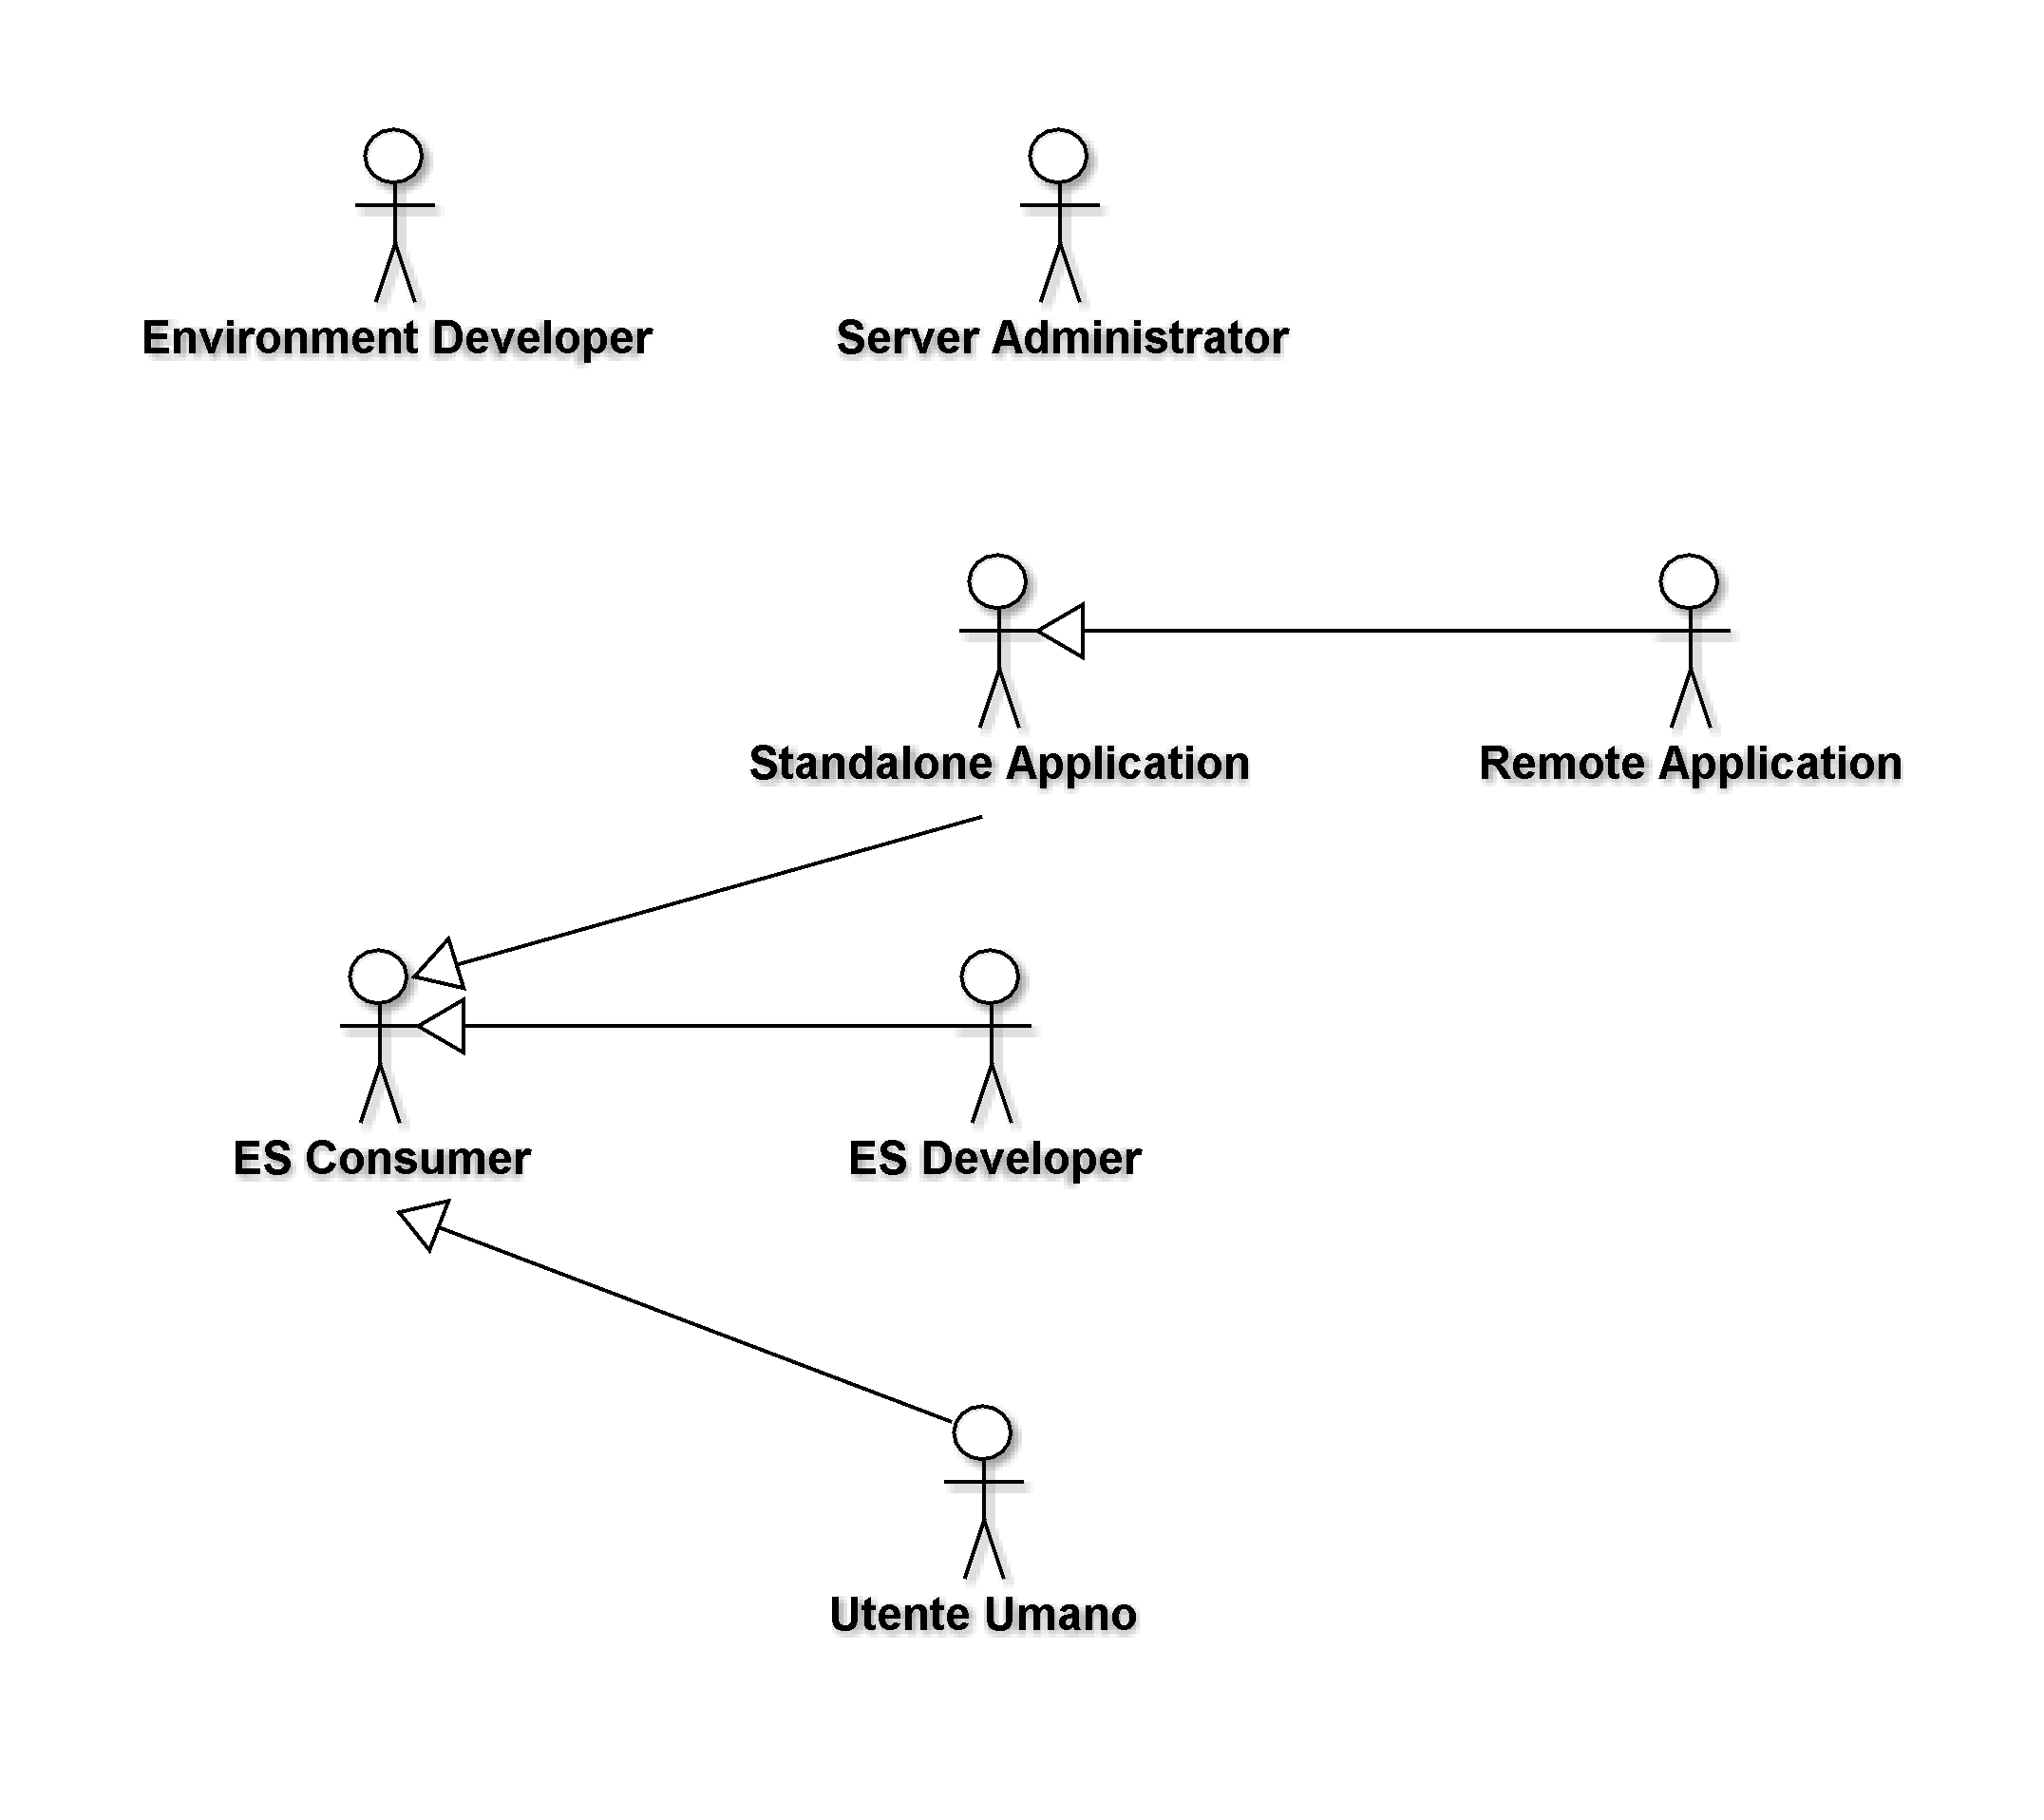
\includegraphics[width=0.9\textwidth]{Immagini/Capitolo2/UseCases/Attori.png}
\caption{Gerarchia degli attori}\label{fig:attori}
\end{figure}

\begin{description}
	\item[ES Consumer:] rappresenta un attore generalizzato in grado di utilizzare i servizi principali offerti dall'\emph{environment} per caricare, eseguire ed interagire con un artefatto precedentemente creato tramite i protocolli offerti dall'\emph{environment} stesso.
	
	\item[ES Developer:] servendosi del linguaggio di specifica fornito dall'\emph{environment} realizza artefatti eseguibili. Tramite l'utilizzo di apposite interfacce è anche in grado di testare l'artefatto prodotto analizzando rappresentazioni grafiche delle strutture interpretate e registri d'attività dell'esecuzione dell'artefatto.
	\item[Utente Umano]
	
	\item[Standalone Application:] utilizza i servizi offerti dall'\emph{environment} all'interno di applicazioni \emph{stand-alone}. Esegue artefatti e valuta i risultati dell'esecuzione analizzando eventi e lo stato finale del sistema.
	
	\item[Remote Application:] esegue attività analoghe a quelle di \emph{Standalone Application}, ma utilizzando i servizi tramite appositi protocolli di comunicazione. Per supportare questi protocolli l'attore può creare, configurare o distruggere sessioni.
	
	\item[Environment Developer:] utilizzando la documentazione di sistema e le apposite \emph{API} fornite, estende le funzionalità dell'\emph{environment} aggiungendo nuove funzioni di sistema, strategie di risoluzione dei conflitti o \emph{event-listener}. Utilizzando un framework per l'esecuzione di test d'unità, può verificare il funzionamento delle funzioni integrate.
	
	\item[Server Administrator:] configura e gestisce un'istanza server dell'\emph{en\-vi\-ron\-ment}.
	
\end{description}

\subsection{Organizzazione dei Casi d'uso}

\begin{figure}
\centering
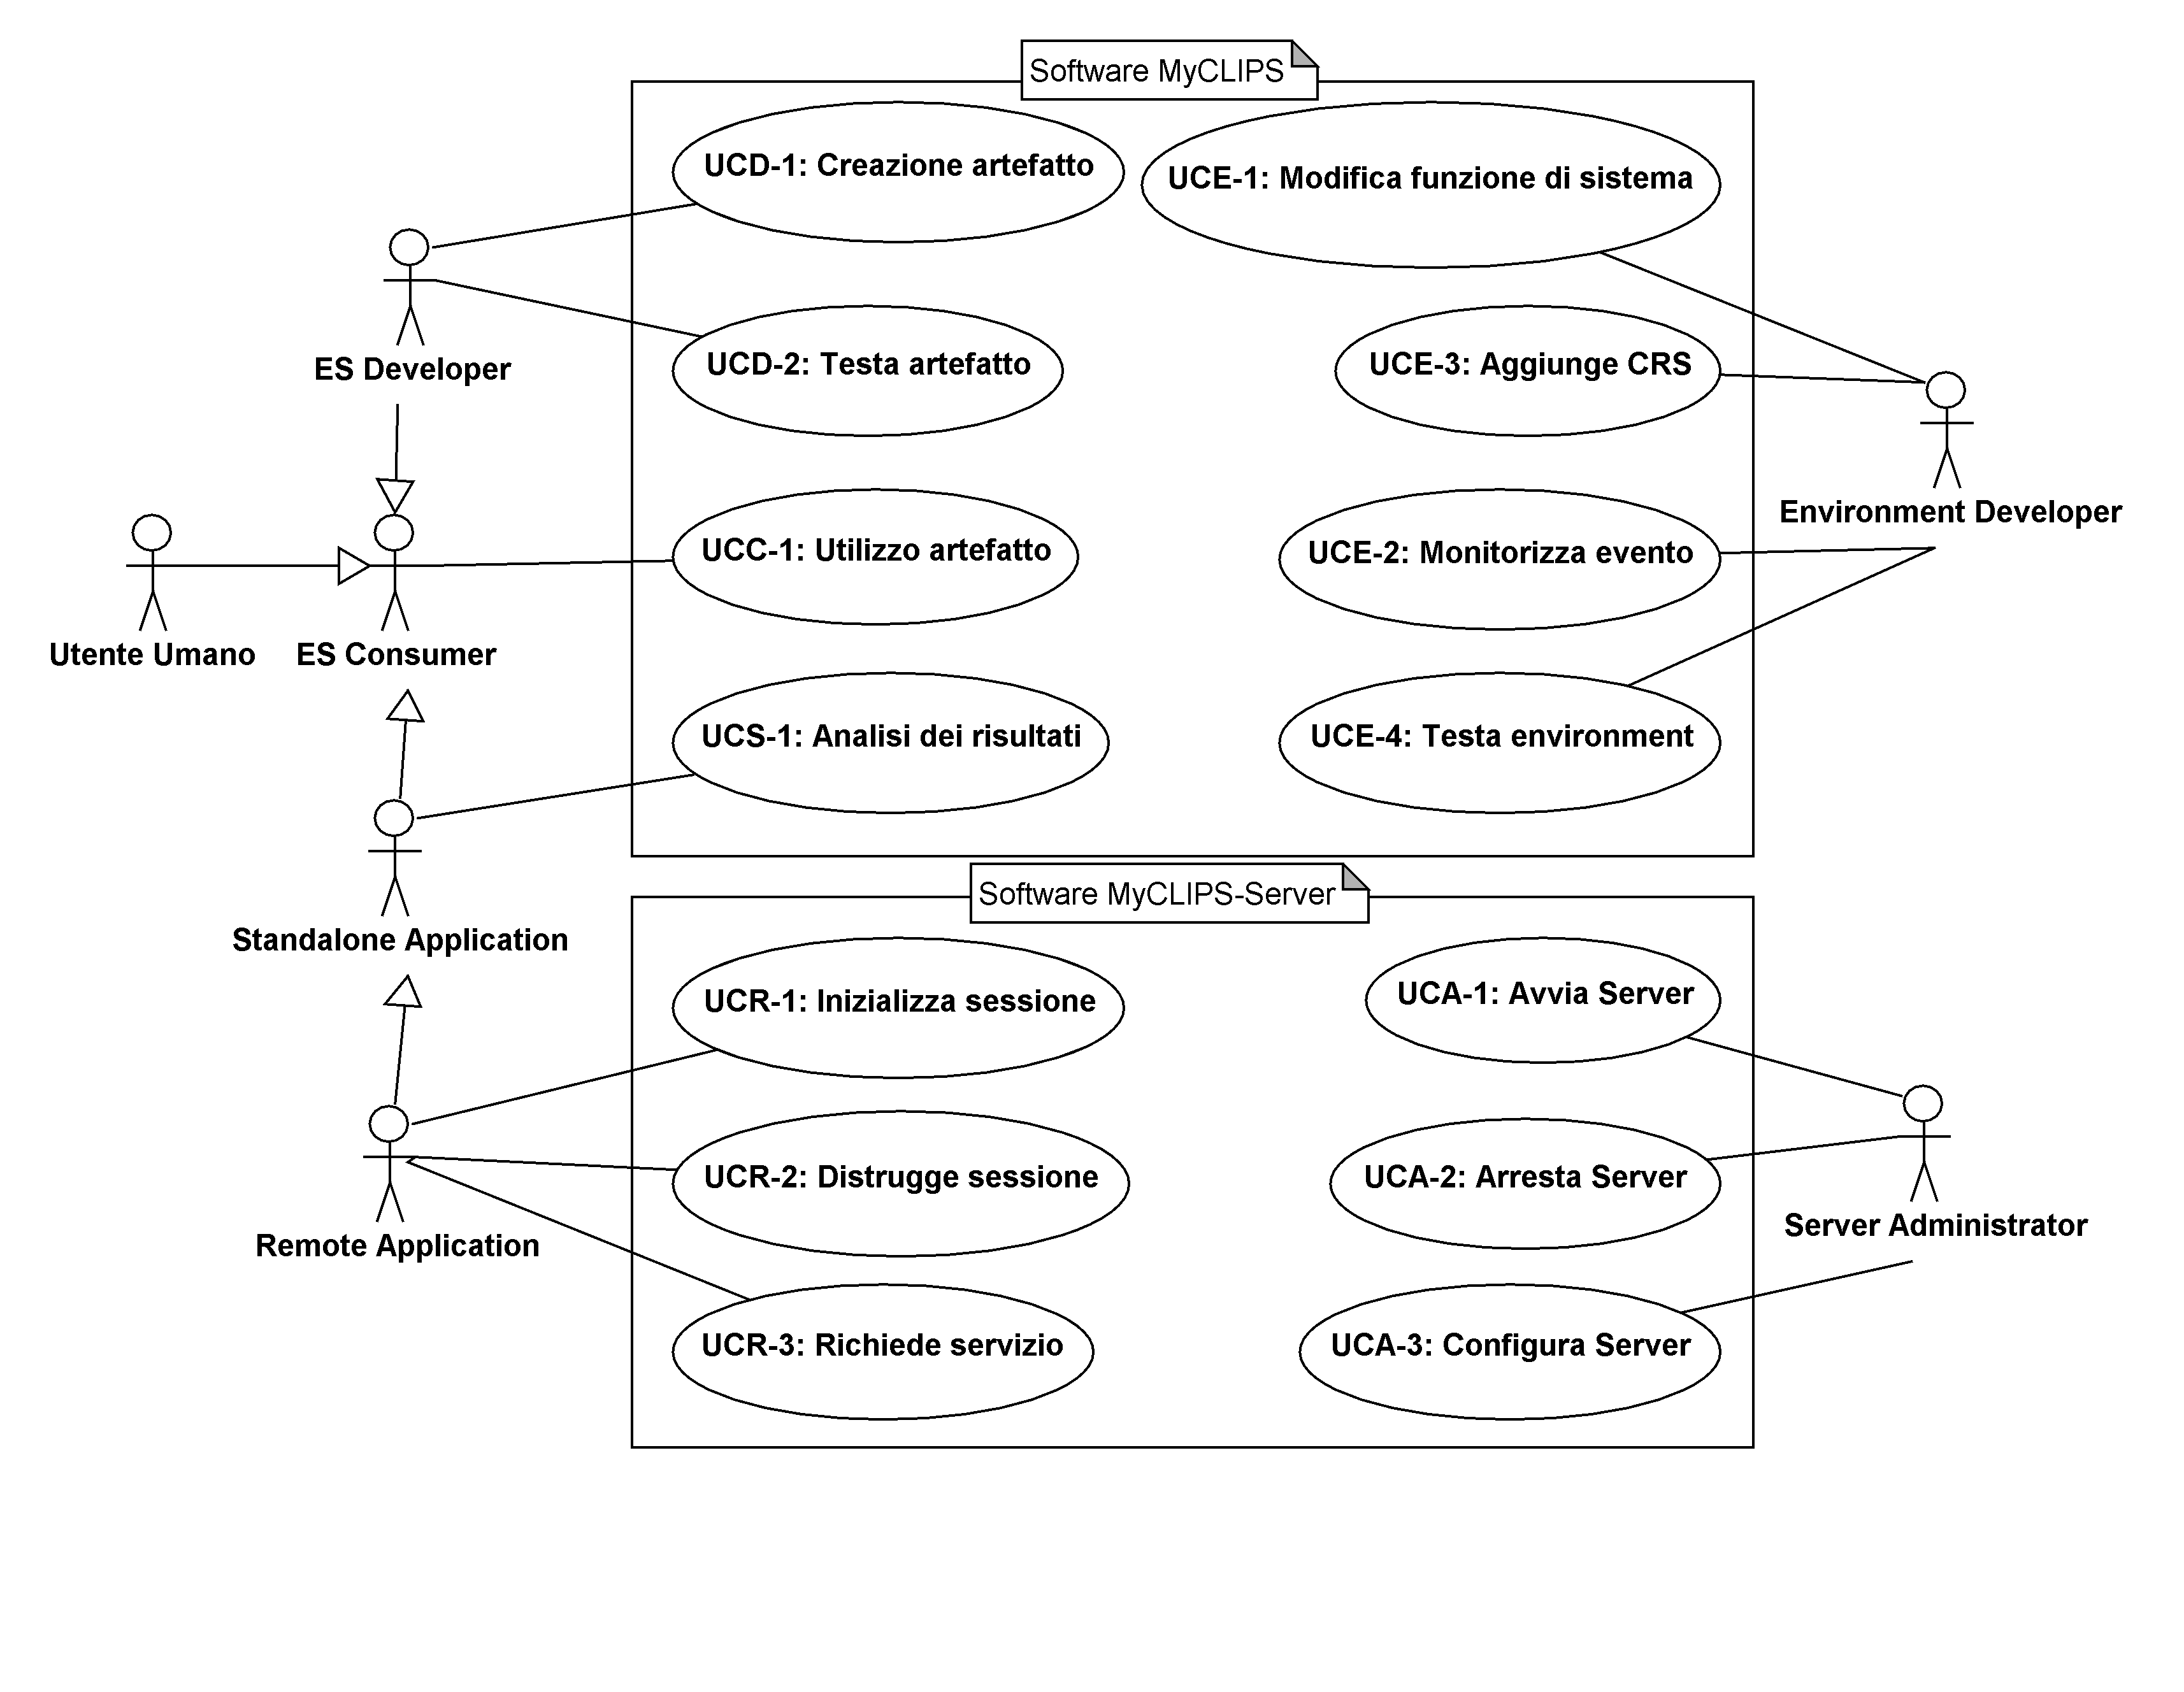
\includegraphics[width=1.2\textwidth, angle=270]{Immagini/Capitolo2/UseCases/Vista-generale.png}
\caption{Vista generale dei casi d'uso principali}\label{fig:uc-vista-generale}
\end{figure}


I casi d'uso vengono organizzati in quattro gruppi  (\figurename~\ref{fig:uc-vista-generale}). Il gruppo di appartenenza di ognuno, indicato dal prefisso inserito nel nome, viene associato tenendo conto dell'attore principale al quale l'\emph{use case} fa riferimento. Il formato del nome di ogni caso d'uso seguirà quindi questa convenzione:
\begin{center}
UC[\emph{Attore}]-[\emph{Sezione}].[\emph{Gruppo}].[\emph{SottoGruppo}]: [\emph{Descrizione breve}]
\end{center}
dove:


\begin{description}
	\item[Attore] indica l'attore principale relazionato con il caso d'uso: \textbf{E} per \emph{Environment Developer}, \textbf{A} per \emph{Server Administrator}, \textbf{S} per \emph{Standalone Application}, \textbf{R} per \emph{Remote Application}, \textbf{D} per \emph{ES Developer} e \textbf{C} per \emph{ES Consumer}. Non è presente nessuno codice per l'attore \emph{Utente umano} in quanto non esiste alcun caso d'uso relativo esclusivamente ad esso.

	\item[Sezione] indica una delle sezioni principali presenti nella vista generale fornita in \figurename~\ref{fig:uc-vista-generale}.
	
	\item[Gruppo] e \textbf{SottoGruppo} esplicitano un'organizzazione gerarchica dei casi d'uso.

\end{description}

\pagebreak

\subsubsection{UCC-1: Utilizzo artefatto}

%UCC-1: Utilizzo artefatto

\begin{figure}
\centering
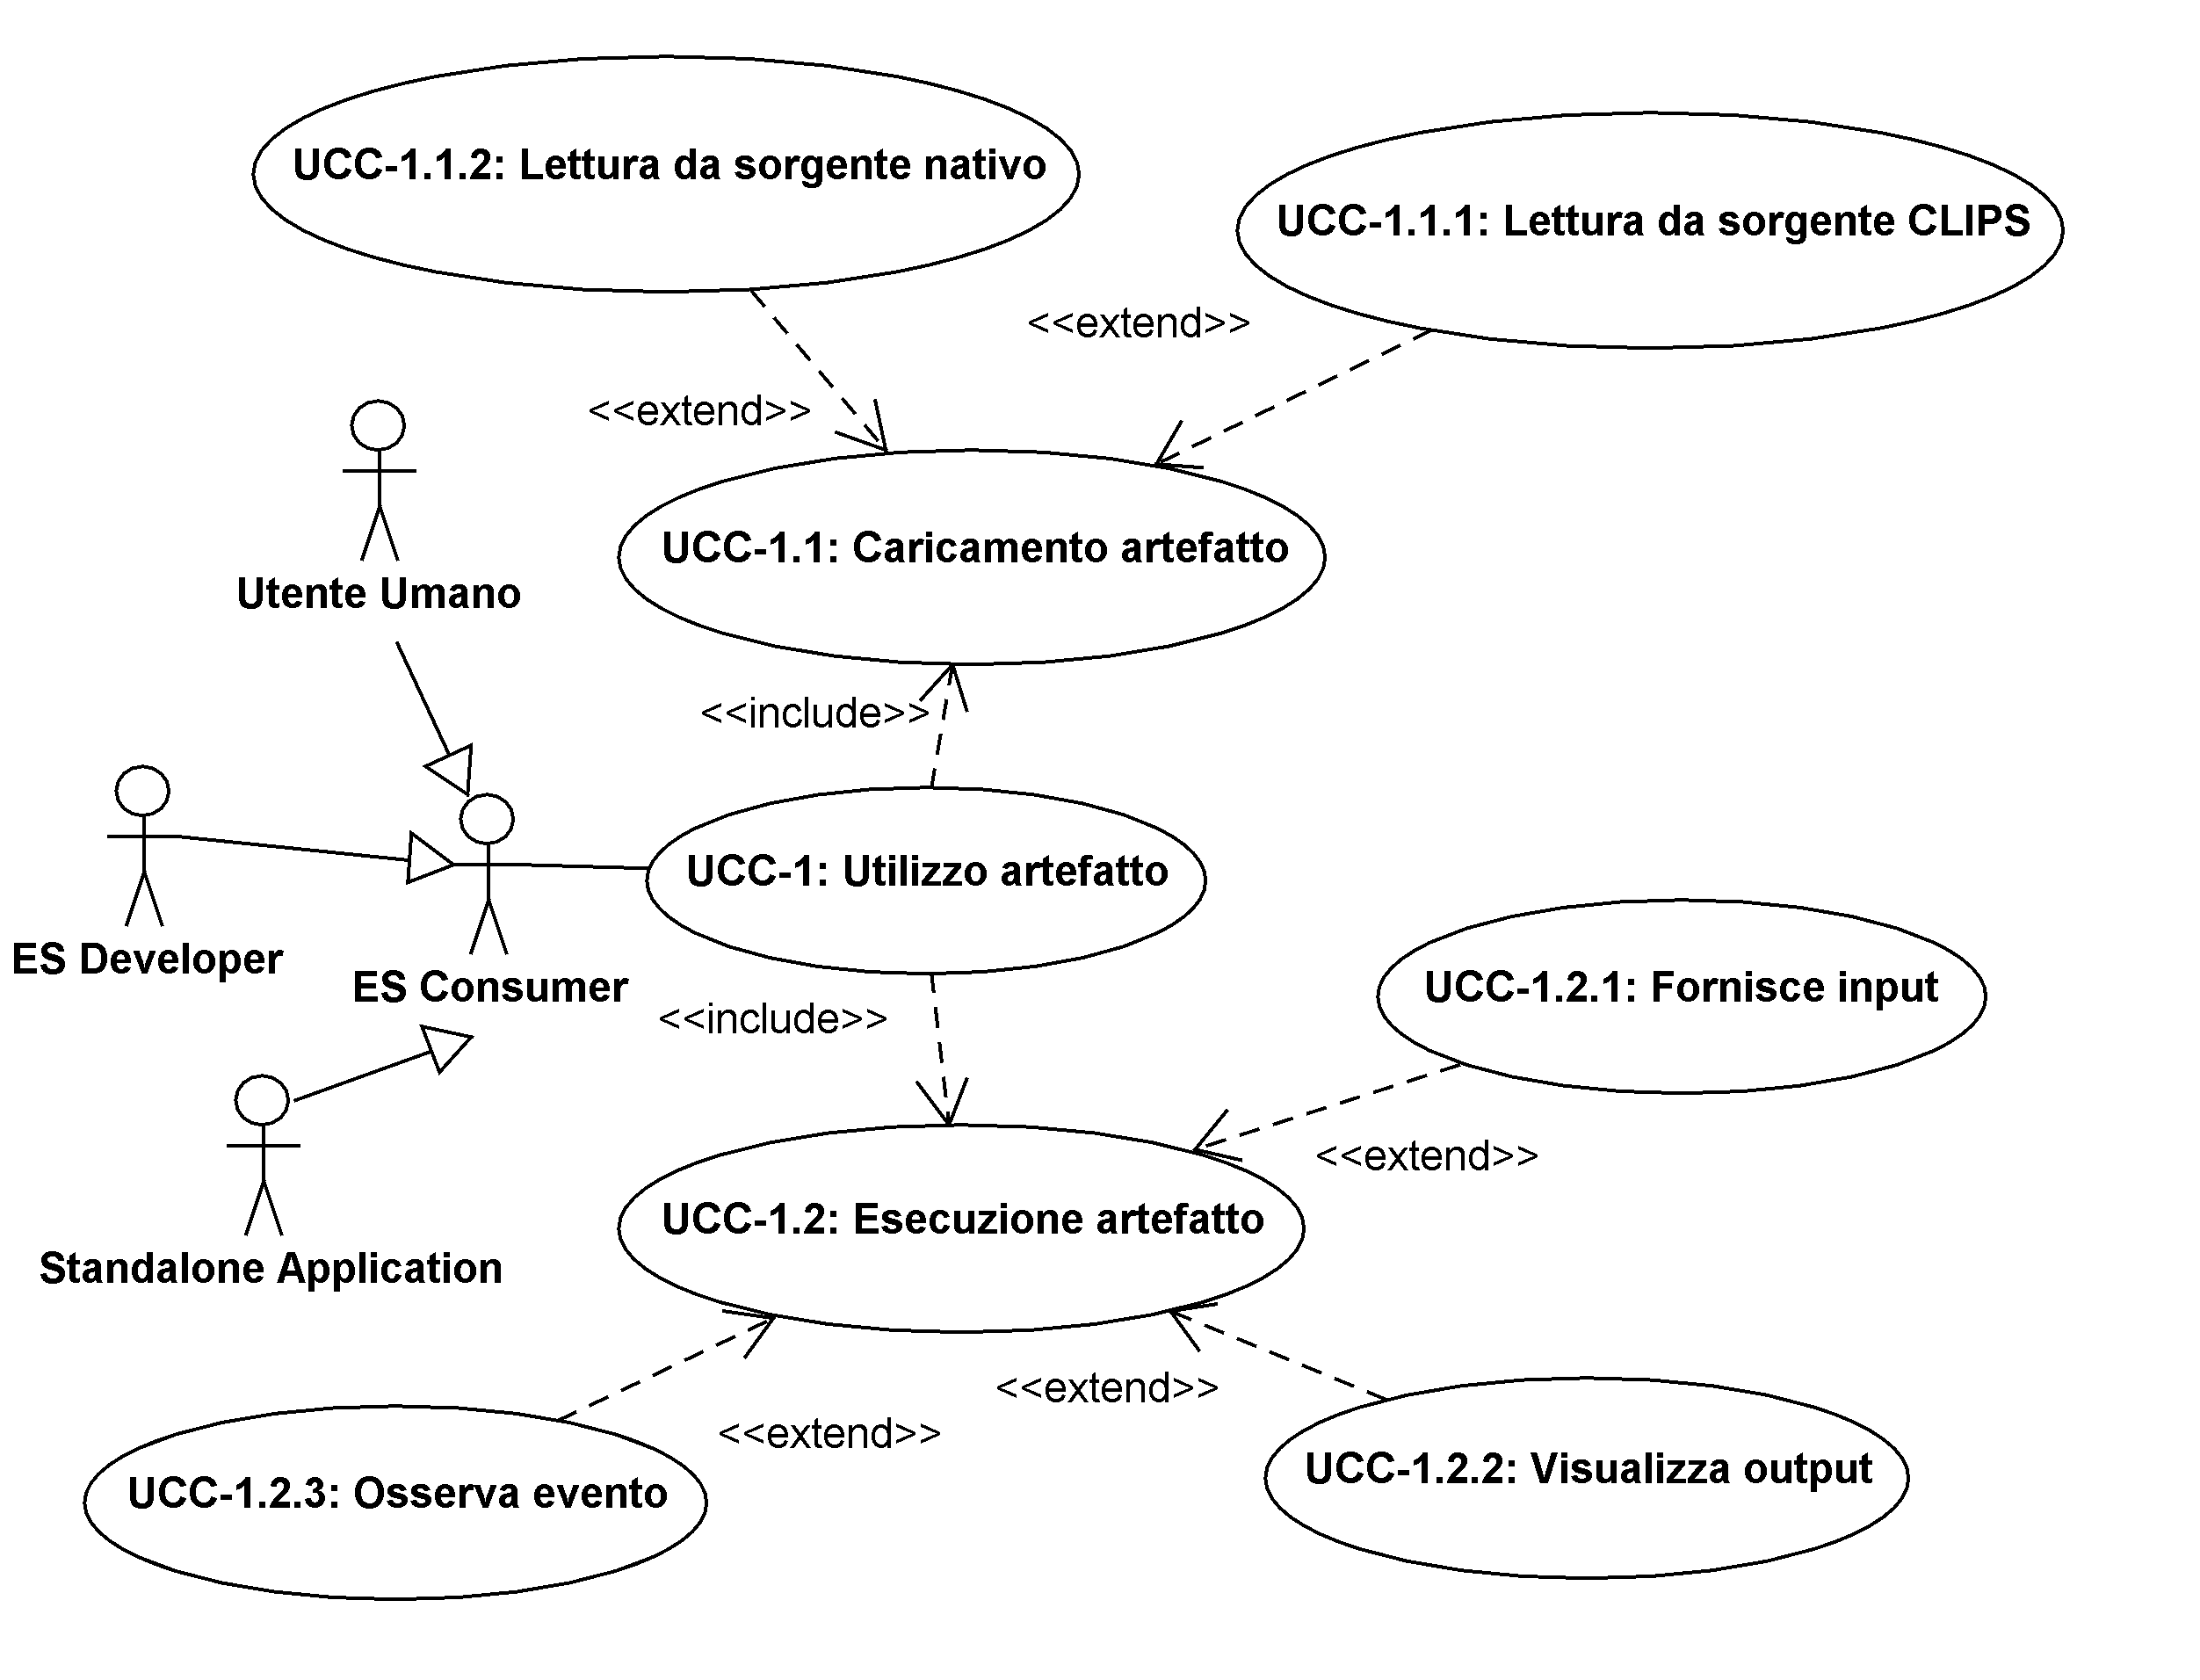
\includegraphics[width=1\textwidth]{Immagini/Capitolo2/UseCases/UCC-1.png}
\caption{Diagramma dei casi d'uso UCC-1}\label{fig:uc-ucc-1}
\end{figure}


\begin{itemize}
	\item \textbf{Attori:} ES Consumer
	\item \textbf{Scopo e descrizione:} un ES Consumer deve poter utilizzare un artefatto precedentemente creato, caricandolo e successivamente eseguendolo.
	\item \textbf{Pre-condizioni:} il software è correttamente configurato nel sistema
	\item \textbf{Post-condizioni:} il software ha eseguito tutte le operazioni desiderate
	\item \textbf{Flusso principale degli eventi:}
		\begin{enumerate}
			\item l'ES Consumer richiede al software di effettuare il caricamento di un artefatto (si veda caso d'uso \emph{UCC-1.1}).
			\item l'ES Consumer richiede al software di eseguire un artefatto (si veda caso d'uso \emph{UCC-1.2}).
		\end{enumerate}
\end{itemize}


\paragraph{UCC-1.1: Caricamento artefatto}

La descrizione comprende quelle dei casi d'uso \emph{UCC-1.1.1} e \emph{UCC-1.1.2} in quanto identici, a meno del formato con il quale l'artefatto viene fornito.

\begin{itemize}
	\item \textbf{Attori:} ES Consumer
	\item \textbf{Scopo e descrizione:} un ES Consumer deve avere la possibilità di caricare nel sistema un artefatto formalizzato in codice sorgente nativo o codice sorgente CLIPS
	\item \textbf{Pre-condizioni:} il software è correttamente configurato nel sistema
	\item \textbf{Post-condizioni:} il software ha eseguito le operazioni di caricamento ed il suo stato rispecchia quello descritto nell'artefatto
	\item \textbf{Flusso principale degli eventi:}
		\begin{enumerate}
			\item l'ES Consumer richiede al software di caricare un artefatto
			\begin{itemize}
				\item l'ES Consumer può fornire un artefatto in formato nativo
				\item l'ES Consumer può fornire un artefatto in formatto CLIPS
			\end{itemize}
			\item Il software analizza l'artefatto
			\item Il software esegue il caricamento dei costrutti contenuti nell'artefatto
		\end{enumerate}
	\item \textbf{Flusso alternativo:}
		\begin{enumerate}
			\setcounter{enumi}{2}
			\item se l'ES Consumer ha fornito un artefatto in formato non valido, il software notifica l'errore fornendo la motivazione e la posizione del problema
		\end{enumerate}
\end{itemize}

\paragraph{UCC-1.2: Esecuzione artefatto}

\begin{itemize}
	\item \textbf{Attori:} ES Consumer
	\item \textbf{Scopo e descrizione:} l'ES Consumer deve poter eseguire un artefatto caricato nel sistema. Se l'interazione lo richiede, l'ES Consumer deve essere in grado di fornire informazioni aggiuntive, osservare l'accadimento di un evento e osservare l'output fornito dal sistema
	\item \textbf{Pre-condizioni:} il software ha correttamente caricato un artefatto ed attende istruzioni.
	\item \textbf{Post-condizioni:} il software ha correttamente eseguito le operazioni previste dall'artefatto.
	\item \textbf{Flusso principale degli eventi:}
		\begin{enumerate}
			\item l'ES Consumer richiede l'esecuzione di un artefatto
			\item il sistema esegue le operazioni previste dall'artefatto (si vedano i casi d'uso \emph{UCC-1.2.1}, \emph{UCC-1.2.3})
			\item il sistema fornisce all'ES Consumer i risultati dell'esecuzione		
		\end{enumerate}
	\item \textbf{Flusso alternativo:} 
		\begin{enumerate}
			\setcounter{enumi}{1}
			\item se un'operazione specificata nell'artefatto genera errori, il sistema notifica l'errore all'ES Consumer fornendo informazioni sulla natura del problema.
			\item il sistema ritorna nello stato iniziale
		\end{enumerate}
\end{itemize}


\subparagraph{UCC-1.2.1: Fornisce input}

\begin{itemize}
	\item \textbf{Attori:} ES Consumer
	\item \textbf{Scopo e descrizione:} l'ES Consumer fornisce informazioni aggiuntive 
	\item \textbf{Pre-condizioni:} il sistema richiede informazioni aggiuntive per completare l'esecuzione di un artefatto
	\item \textbf{Post-condizioni:} il sistema prosegue l'esecuzione
	\item \textbf{Flusso principale degli eventi:}
		\begin{enumerate}
			\item il sistema richiede informazioni aggiuntive
			\item l'ES Consumer fornisce le informazioni nelle forme previste dall'artefatto
			\item il sistema valuta le informazioni fornite
			\item il sistema elabora le informazioni fornite
		\end{enumerate}
	\item \textbf{Flusso alternativo:} 
		\begin{enumerate}
			\setcounter{enumi}{2}
			\item il sistema notifica l'invalidità delle informazioni fornite
			\item il flusso riprende dal punto 1 del flusso principale
		\end{enumerate}
\end{itemize}


\subparagraph{UCC-1.2.2: Visualizza output}

\begin{itemize}
	\item \textbf{Attori:} ES Consumer
	\item \textbf{Scopo e descrizione:} l'ES Consumer deve essere in grado di valutare l'output fornito dal sistema al termine di un'operazione
	\item \textbf{Pre-condizioni:} il sistema è pronto ad esegue un'operazione
	\item \textbf{Post-condizioni:} il sistema è pronto ad eseguire una nuova operazione
	\item \textbf{Flusso principale degli eventi:}
		\begin{enumerate}
			\item il sistema esegue un'operazione
			\item il sistema fornisce una visualizzazione del risultato
			\item l'ES Consumer valuta il risultato
		\end{enumerate}
\end{itemize}


\subparagraph{UCC-1.2.3: Osserva evento}

\begin{itemize}
	\item \textbf{Attori:} ES Consumer
	\item \textbf{Scopo e descrizione:} l'ES Consumer deve essere in grado di ricevere notifica del verificarsi di un evento
	\item \textbf{Pre-condizioni:} il sistema è pronto ad eseguire un'operazione
	\item \textbf{Post-condizioni:} il sistema è pronto ad eseguire un'operazione
	\item \textbf{Flusso principale degli eventi:}
		\begin{enumerate}
			\item l'ES Consumer richiede al sistema di eseguire un'operazione
			\item il sistema esegue un'operazione
			\item il sistema notifica all'ES Consumer il verificarsi di un evento
			\item l'ES Consumer valuta l'evento
		\end{enumerate}
\end{itemize}\pagebreak

\subsubsection{UCD-1: Creazione artefatto}

%UCD-1: Creazione artefatto

\begin{figure}
\centering
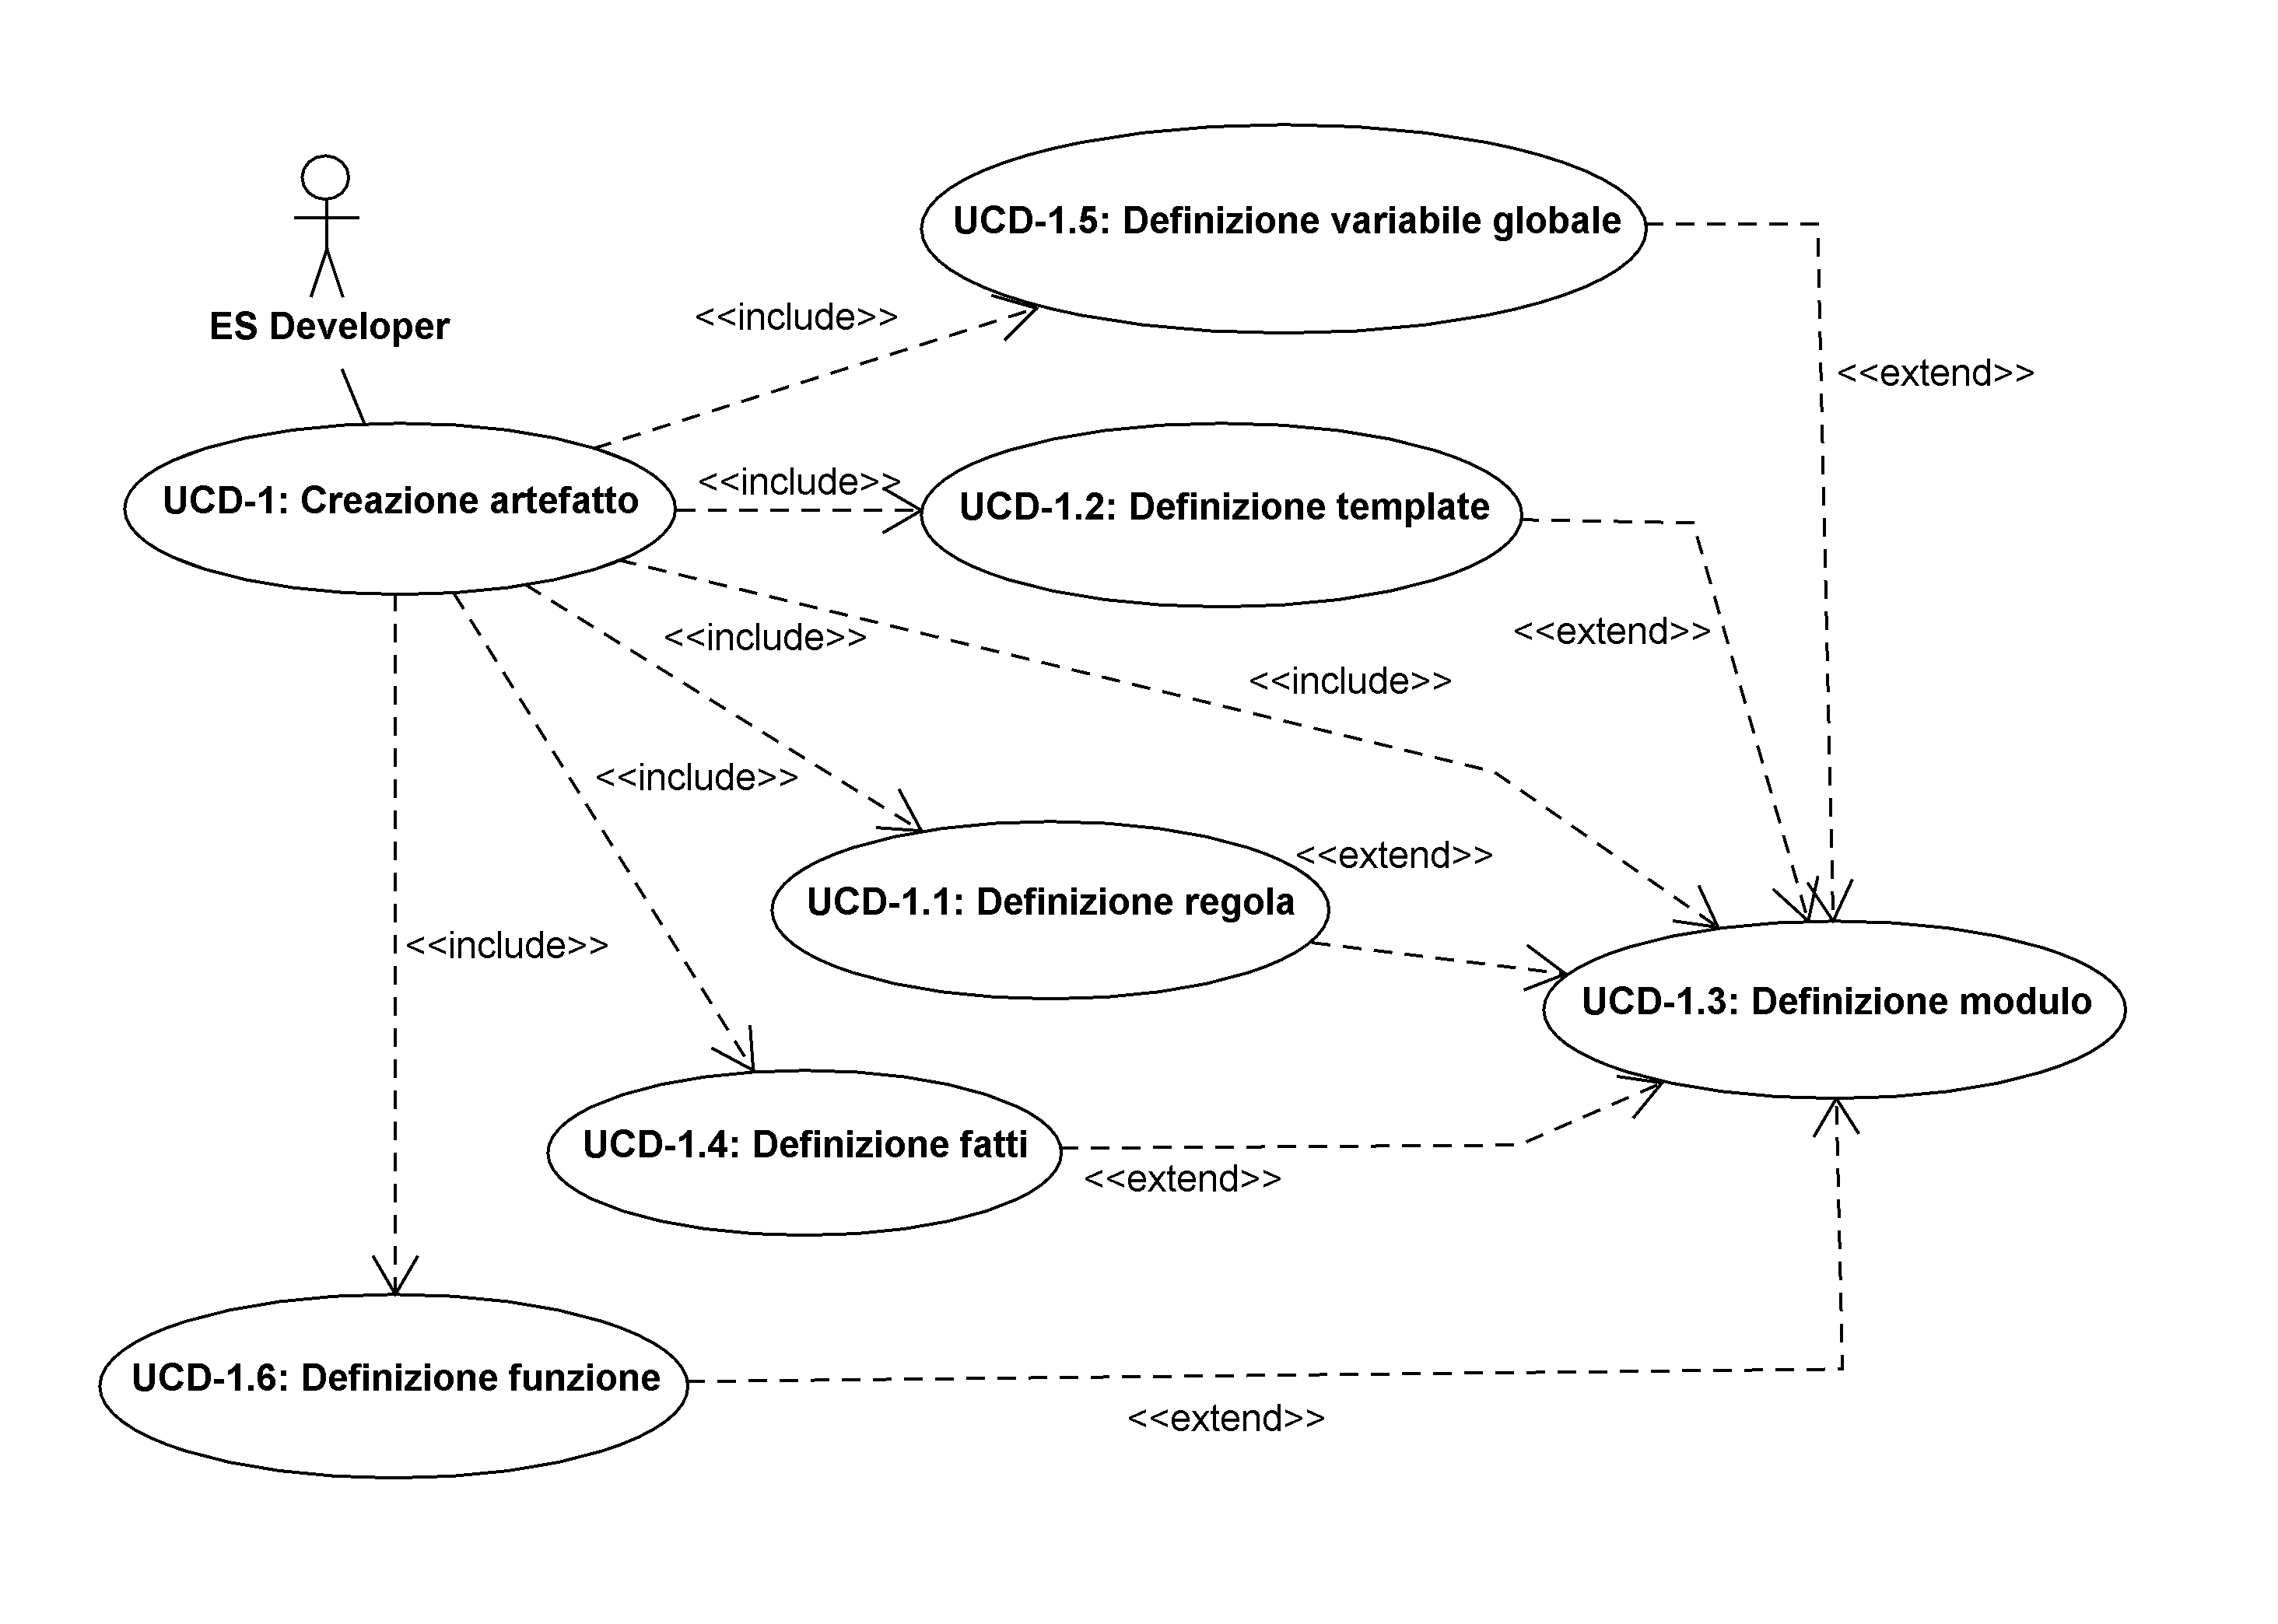
\includegraphics[width=1.1\textwidth]{Immagini/Capitolo2/UseCases/UCD-1.png}
\caption{Diagramma dei casi d'uso UCD-1}\label{fig:uc-ucd-1}
\end{figure}


\begin{itemize}
	\item \textbf{Attori:} ES Developer
	\item \textbf{Scopo e descrizione:} un ES Developer deve essere in grado di definire i costrutti necessari alla realizzazione di un artefatto.
	\item \textbf{Pre-condizioni:} il software fornisce almeno un linguaggio di specifica
	\item \textbf{Post-condizioni:} un artefatto è stato serializzato tramite il linguaggio di specifica
	\item \textbf{Flusso principale degli eventi:}
		\begin{enumerate}
			\item l'ES Developer definisce una serie di costrutti (si vedano i casi d'uso \emph{UCD-1.1}, \emph{UCD-1.2}, \emph{UCD-1.3}, \emph{UCD-1.4}, \emph{UCD-1.5}, \emph{UCD-1.6}).
			\begin{itemize}
				\item l'ES Developer può formalizzarlo in formato nativo
				\item l'ES Developer può formalizzarlo in formatto CLIPS
			\end{itemize}
			\item l'ES Consumer verifica la correttezza dell'artefatto (si veda il caso d'uso \emph{UCD-1.2}).
		\end{enumerate}
\end{itemize}


\paragraph{UCD-1.1: Definizione regola}

\begin{itemize}
	\item \textbf{Attori:} ES Developer
	\item \textbf{Scopo e descrizione:} un ES Developer deve essere in grado di definire una regola tramite un linguaggio di specifica fornito dal sistema.
	\item \textbf{Pre-condizioni:} il software fornisce almeno un linguaggio di specifica
	\item \textbf{Post-condizioni:} la definizione di una regola è stata aggiunta ad un artefatto
	\item \textbf{Flusso principale degli eventi:}
		\begin{enumerate}
			\item l'ES Developer definisce una regola
			\begin{itemize}
				\item l'ES Developer può formalizzarli in formato nativo
				\item l'ES Developer può formalizzarli in formatto CLIPS
			\end{itemize}
		\end{enumerate}
	\item \textbf{Flusso alternativo:}
		\begin{enumerate}
			\item se l'ES Developer ha definito precedentemente un modulo, l'ES Developer può definire una regola come componente del modulo.
		\end{enumerate}
\end{itemize}


\paragraph{UCD-1.2: Definizione template}

\begin{figure}[h]
\centering
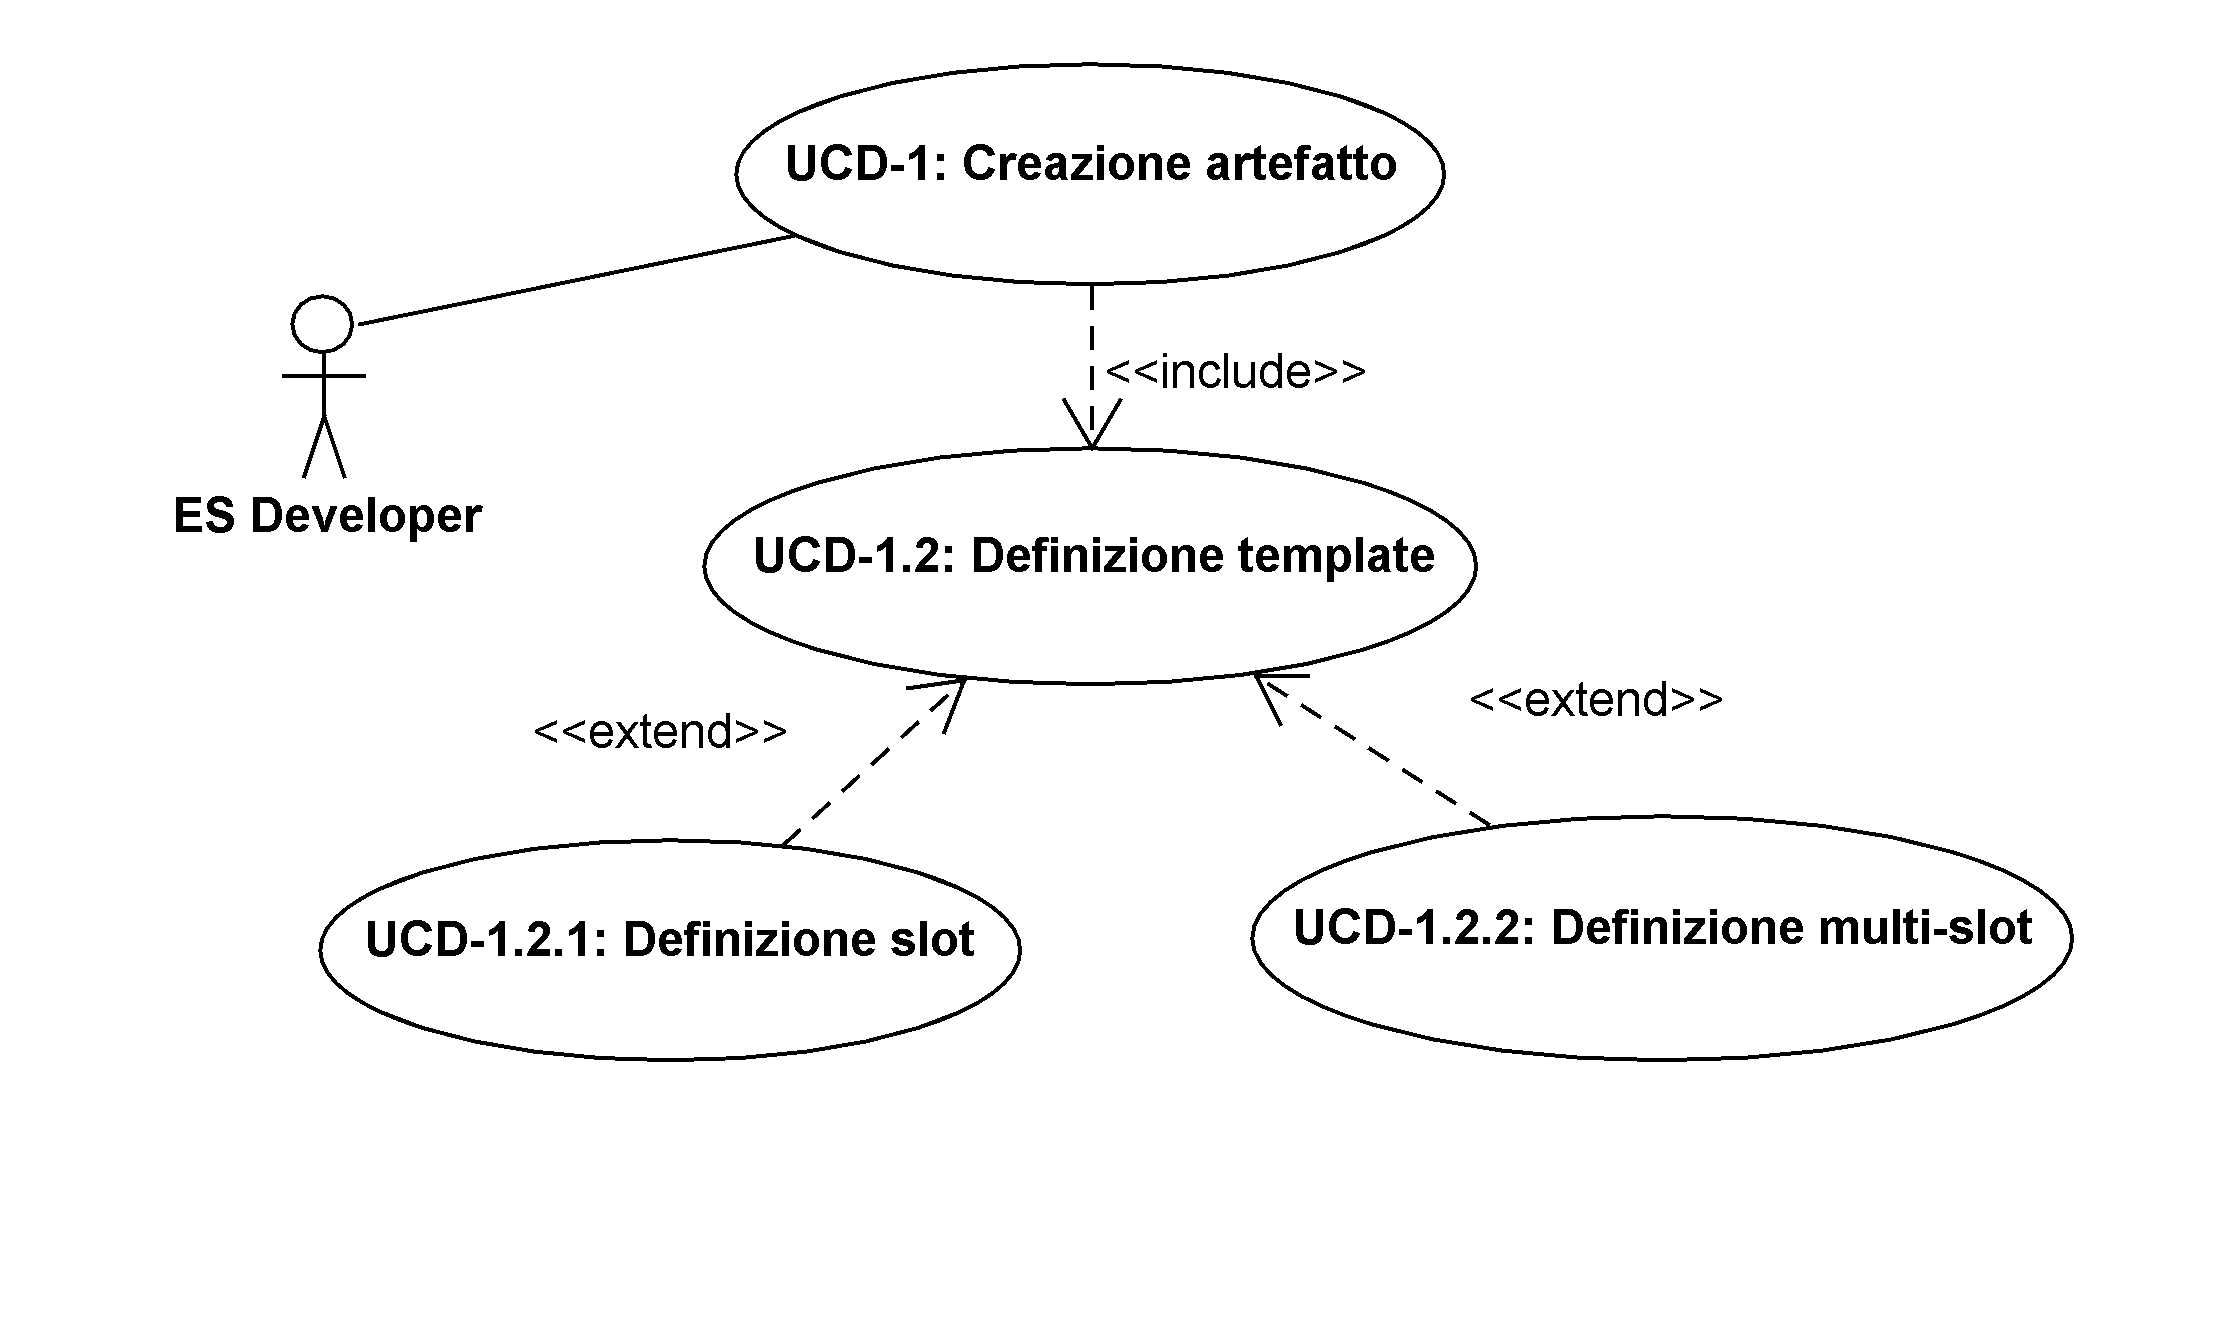
\includegraphics[width=1\textwidth]{Immagini/Capitolo2/UseCases/UCD-1_2.png}
\caption{Diagramma dei casi d'uso UCD-1.2}\label{fig:uc-ucd-1.2}
\end{figure}

\begin{itemize}
	\item \textbf{Attori:} ES Developer
	\item \textbf{Scopo e descrizione:} l'ES Developer deve essere in grado di definire un template di fatti tramite un linguaggio di specifica fornito dal sistema.
	\item \textbf{Pre-condizioni:} il software fornisce almeno un linguaggio di specifica.
	\item \textbf{Post-condizioni:} la definizione di un template di fatti è stato aggiunto ad un artefatto
	\item \textbf{Flusso principale degli eventi:}
		\begin{enumerate}
			\item l'ES Developer definisce un template di fatti
			\item l'ES Developer definisce il formato del template di fatti (si vedano i casi d'uso \emph{UCD-1.2.1}, \emph{UCD-1.2.2})
		\end{enumerate}
	\item \textbf{Flusso alternativo:} 
		\begin{enumerate}
			\item se l'ES Developer ha definito precedentemente un modulo, l'ES Developer può definire un template di fatti come componente di un modulo
		\end{enumerate}
\end{itemize}

\subparagraph{UCD-1.2.1: Definizione slot}

\begin{itemize}
	\item \textbf{Attori:} ES Developer
	\item \textbf{Scopo e descrizione:} l'ES Developer deve essere in grado di definire il formato di uno slot appartenente ad un template di fatti
	\item \textbf{Pre-condizioni:} il software fornisce un linguaggio di specifica, l'ES developer ha definito un template di fatti
	\item \textbf{Post-condizioni:} il formato dello slot è stato aggiunto alla definizione di template di fatti
	\item \textbf{Flusso principale degli eventi:}
		\begin{enumerate}
			\item l'ES Developer definisce un template
			\item l'ES Developer definisce un nuovo slot fornendo il nome (stringa alfanumerica) da attribuire allo stesso
			\begin{enumerate}
				\item l'ES Developer può definire una restrizione di tipo al contenuto dello slot
				\item l'ES Developer può definire un valore di \emph{default} per lo slot
			\end{enumerate}
		\end{enumerate}
	\item \textbf{Flusso alternativo:} 
		\begin{enumerate}
			\setcounter{enumi}{1}
			\item se l'ES Developer ha fornito un nome già usato da un altro slot o multi-slot presente, il sistema rifiuta la definizione notificando un errore.
		\end{enumerate}
\end{itemize}

\subparagraph{UCD-1.2.2: Definizione multi-slot}

\begin{itemize}
	\item \textbf{Attori:} ES Developer
	\item \textbf{Scopo e descrizione:} l'ES Developer deve essere in grado di definire il formato di un multi-slot appartenente ad un template di fatti
	\item \textbf{Pre-condizioni:} il software fornisce un linguaggio di specifica, l'ES Developer ha definito un template di fatti
	\item \textbf{Post-condizioni:} il formato del multi-slot è stato aggiunto alla definizione di template di fatti
	\item \textbf{Flusso principale degli eventi:}
		\begin{enumerate}
			\item l'ES Developer definisce un template
			\item l'ES Developer definisce un nuovo multi-slot fornendo il nome (stringa alfanumerica) da attribuire allo stesso
			\begin{enumerate}
				\item l'ES Developer può definire delle restrizioni di tipo al contenuto dello slot
				\item l'ES Developer può definire dei valori di \emph{default} per il multi-slot
			\end{enumerate}
		\end{enumerate}
	\item \textbf{Flusso alternativo:} 
		\begin{enumerate}
			\setcounter{enumi}{1}
			\item se l'ES Developer ha fornito un nome già usato da un altro slot o multi-slot presente, il sistema rifiuta la definizione notificando un errore.
		\end{enumerate}
\end{itemize}


\paragraph{UCD-1.3: Definizione modulo}

\begin{figure}[h]
\centering
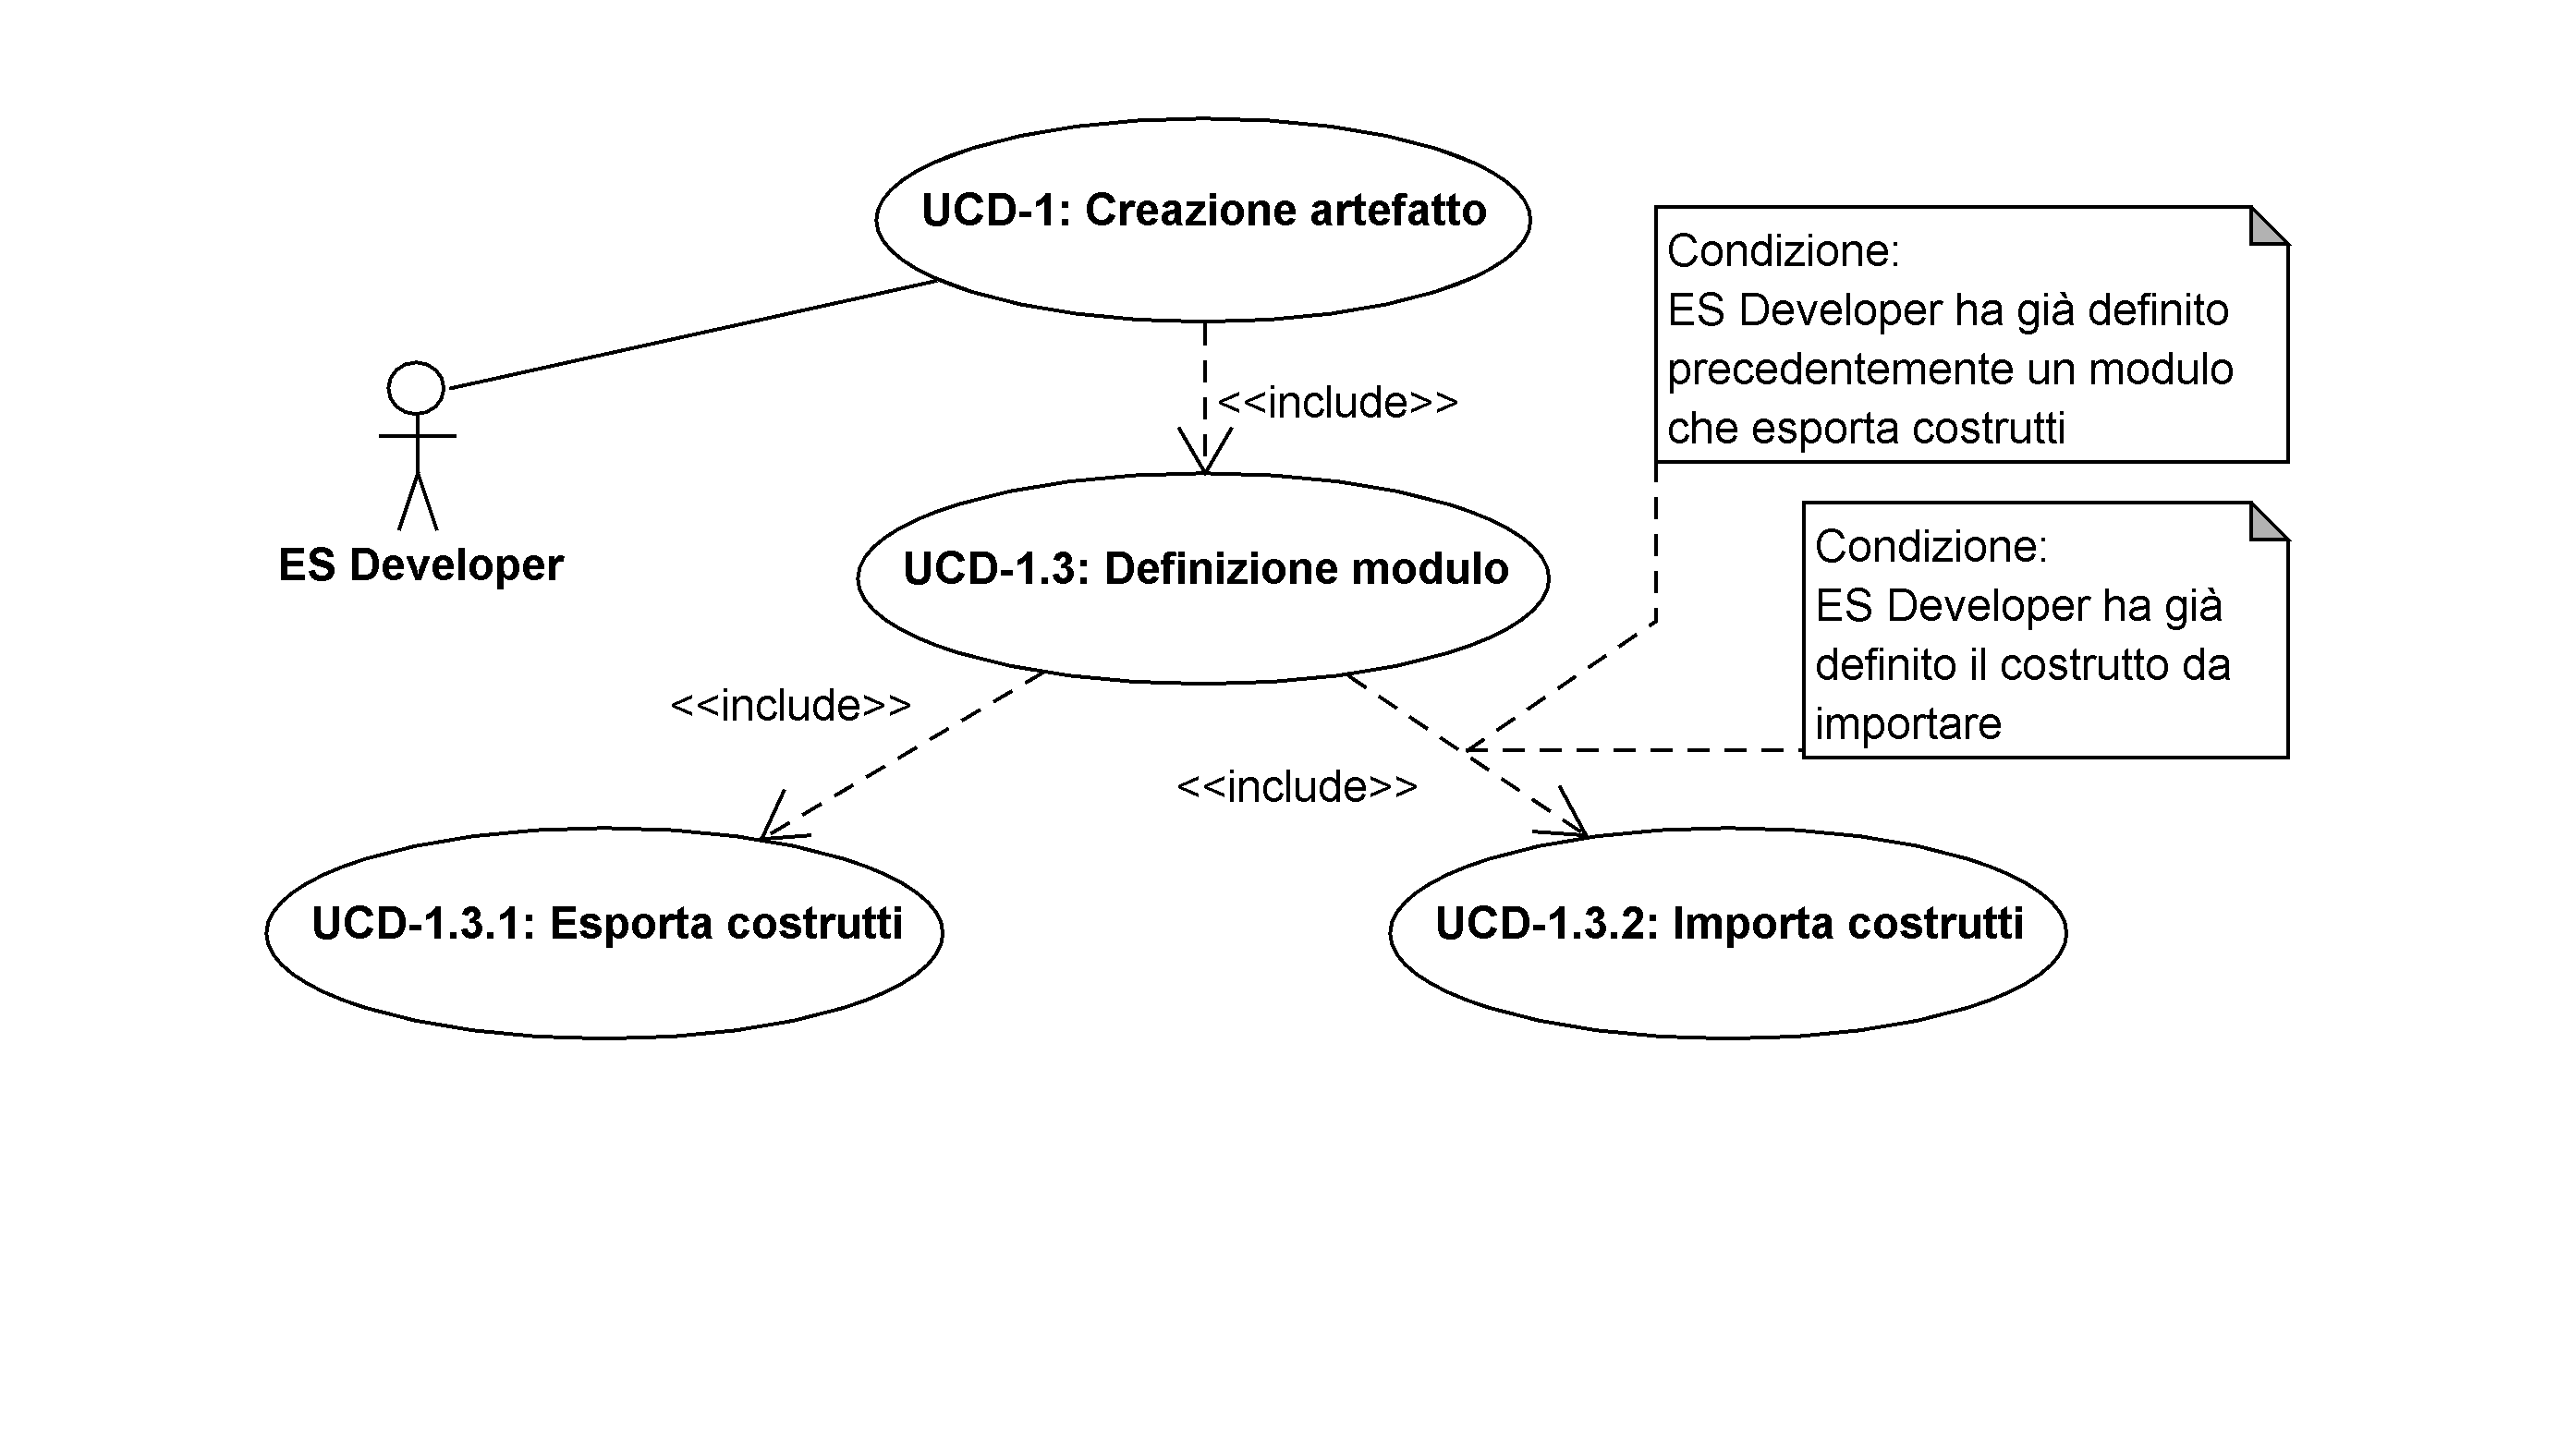
\includegraphics[width=1\textwidth]{Immagini/Capitolo2/UseCases/UCD-1_3.png}
\caption{Diagramma dei casi d'uso UCD-1.3}\label{fig:uc-ucd-1.3}
\end{figure}

\begin{itemize}
	\item \textbf{Attori:} ES Developer
	\item \textbf{Scopo e descrizione:} l'ES Developer deve essere in grado di definire un modulo tramite un linguaggio di specifica fornito dal sistema.
	\item \textbf{Pre-condizioni:} il software fornisce almeno un linguaggio di specifica.
	\item \textbf{Post-condizioni:} la definizione di un modulo è stata aggiunta ad un artefatto.
	\item \textbf{Flusso principale degli eventi:}
		\begin{enumerate}
			\item l'ES Developer definisce un modulo specificandone il nome
			\item l'ES Developer definisce una serie di costrutti da esportare (si veda il caso d'uso \emph{UCD-1.3.1})
			\item l'ES Developer definisce una serie di costrutti da importare da un altro modulo (si veda il caso d'uso \emph{UCD-1.3.2})
		\end{enumerate}
		
	\item \textbf{Flusso alternativo:} 
		\begin{enumerate}
			\setcounter{enumi}{0}
			\item se l'ES Developer fornisce un nome già utilizzato da un altro modulo, il sistema rifiuta la definizione e notifica l'errore.
			\item il sistema ritorna nello stato iniziale.
		\end{enumerate}
		
\end{itemize}

\subparagraph{UCD-1.3.1: Esporta costrutti}

\begin{itemize}
	\item \textbf{Attori:} ES Developer
	\item \textbf{Scopo e descrizione:} l'ES Developer deve essere in grado di specificare l'esportazione di un costrutto relativo al modulo tramite un linguaggio di specifica fornito dal sistema
	\item \textbf{Pre-condizioni:} il sistema fornisce un linguaggio di specifica, l'ES Developer ha definito un modulo
	\item \textbf{Post-condizioni:} il sistema aggiunge il nome del costrutto esportato in un insieme di elementi importabili da altri moduli
	\item \textbf{Flusso principale degli eventi:}
		\begin{enumerate}
			\item l'ES Developer definisce un modulo
			\item l'ES Developer definisce un costrutto appartenente al modulo come esportabile
				\begin{itemize}
					\item l'ES Developer può specificare il nome ed il tipo del costrutto
					\item l'ES Developer può specificare il tipo dei costrutti e un valore speciale per definire l'esportazione di tutti i costrutti del tipo indicato
					\item l'ES Developer può specificare un valore speciale per definire l'esportazione di tutti i costrutti di ogni tipo
					\item l'ES Developer può specificare il tipo ed un valore speciale per definire l'esclusione dei costrutti del tipo specificato dalla lista degli elementi esportati
				\end{itemize}
		\end{enumerate}
\end{itemize}


\subparagraph{UCD-1.3.2: Importa costrutti}

\begin{itemize}
	\item \textbf{Attori:} ES Developer
	\item \textbf{Scopo e descrizione:} l'ES Developer deve essere in grado di specificare l'importazione di un costrutto esportato da un modulo tramite un linguaggio di specifica fornito dal sistema
	\item \textbf{Pre-condizioni:} il sistema fornisce un linguaggio di specifica, l'ES Developer ha definito un modulo che esporta un costrutto, l'ES Developer ha definito un modulo
	\item \textbf{Post-condizioni:} il sistema aggiunge la definizione importata all'insieme di definizione del modulo.
	\item \textbf{Flusso principale degli eventi:}
		\begin{enumerate}
			\item l'ES Developer definisce un modulo
			\item l'ES Developer definisce un costrutto appartenente ad un secondo modulo come importabile.
				\begin{itemize}
					\item l'ES Developer può specificare il modulo, il nome ed il tipo del costrutto da importare
					\item l'ES Developer può specificare il modulo, il tipo ed un valore speciale per definite l'importazione di tutti i costrutti del tipo indicato dal modulo indicato
					\item l'ES Developer può specificare il modulo ed un valore speciale per definire l'importazione di tutti i costrutti dal modulo indicato
					
					\item l'ES Developer può specificare il modulo, il tipo ed un valore speciale per definire l'esclusione di tutti i costrutti del tipo indicato del modulo indicato dall'insieme di costrutti importati
				\end{itemize}
		\end{enumerate}
	\item \textbf{Flusso alternativo \#1:} 
		\begin{enumerate}
			\setcounter{enumi}{1}
			\item se l'ES Developer esegue un'importazione da un modulo non esistente, il sistema rifiuta la definizione e notifica l'errore.
			\item il sistema ritorna nello stato iniziale.
		\end{enumerate}
		
	\item \textbf{Flusso alternativo \#2:} 
		\begin{enumerate}
			\setcounter{enumi}{1}
			\item se l'ES Developer esegue un'importazione di un costrutto non ancora definito da un modulo che lo esporta preventivamente, il sistema rifiuta la definizione e notifica l'errore.
			\item il sistema ritorna nello stato iniziale.
		\end{enumerate}
		
\end{itemize}

\paragraph{UCD-1.4: Definizione fatti} % nome del caso d'uso Gruppo

\begin{figure}
\centering
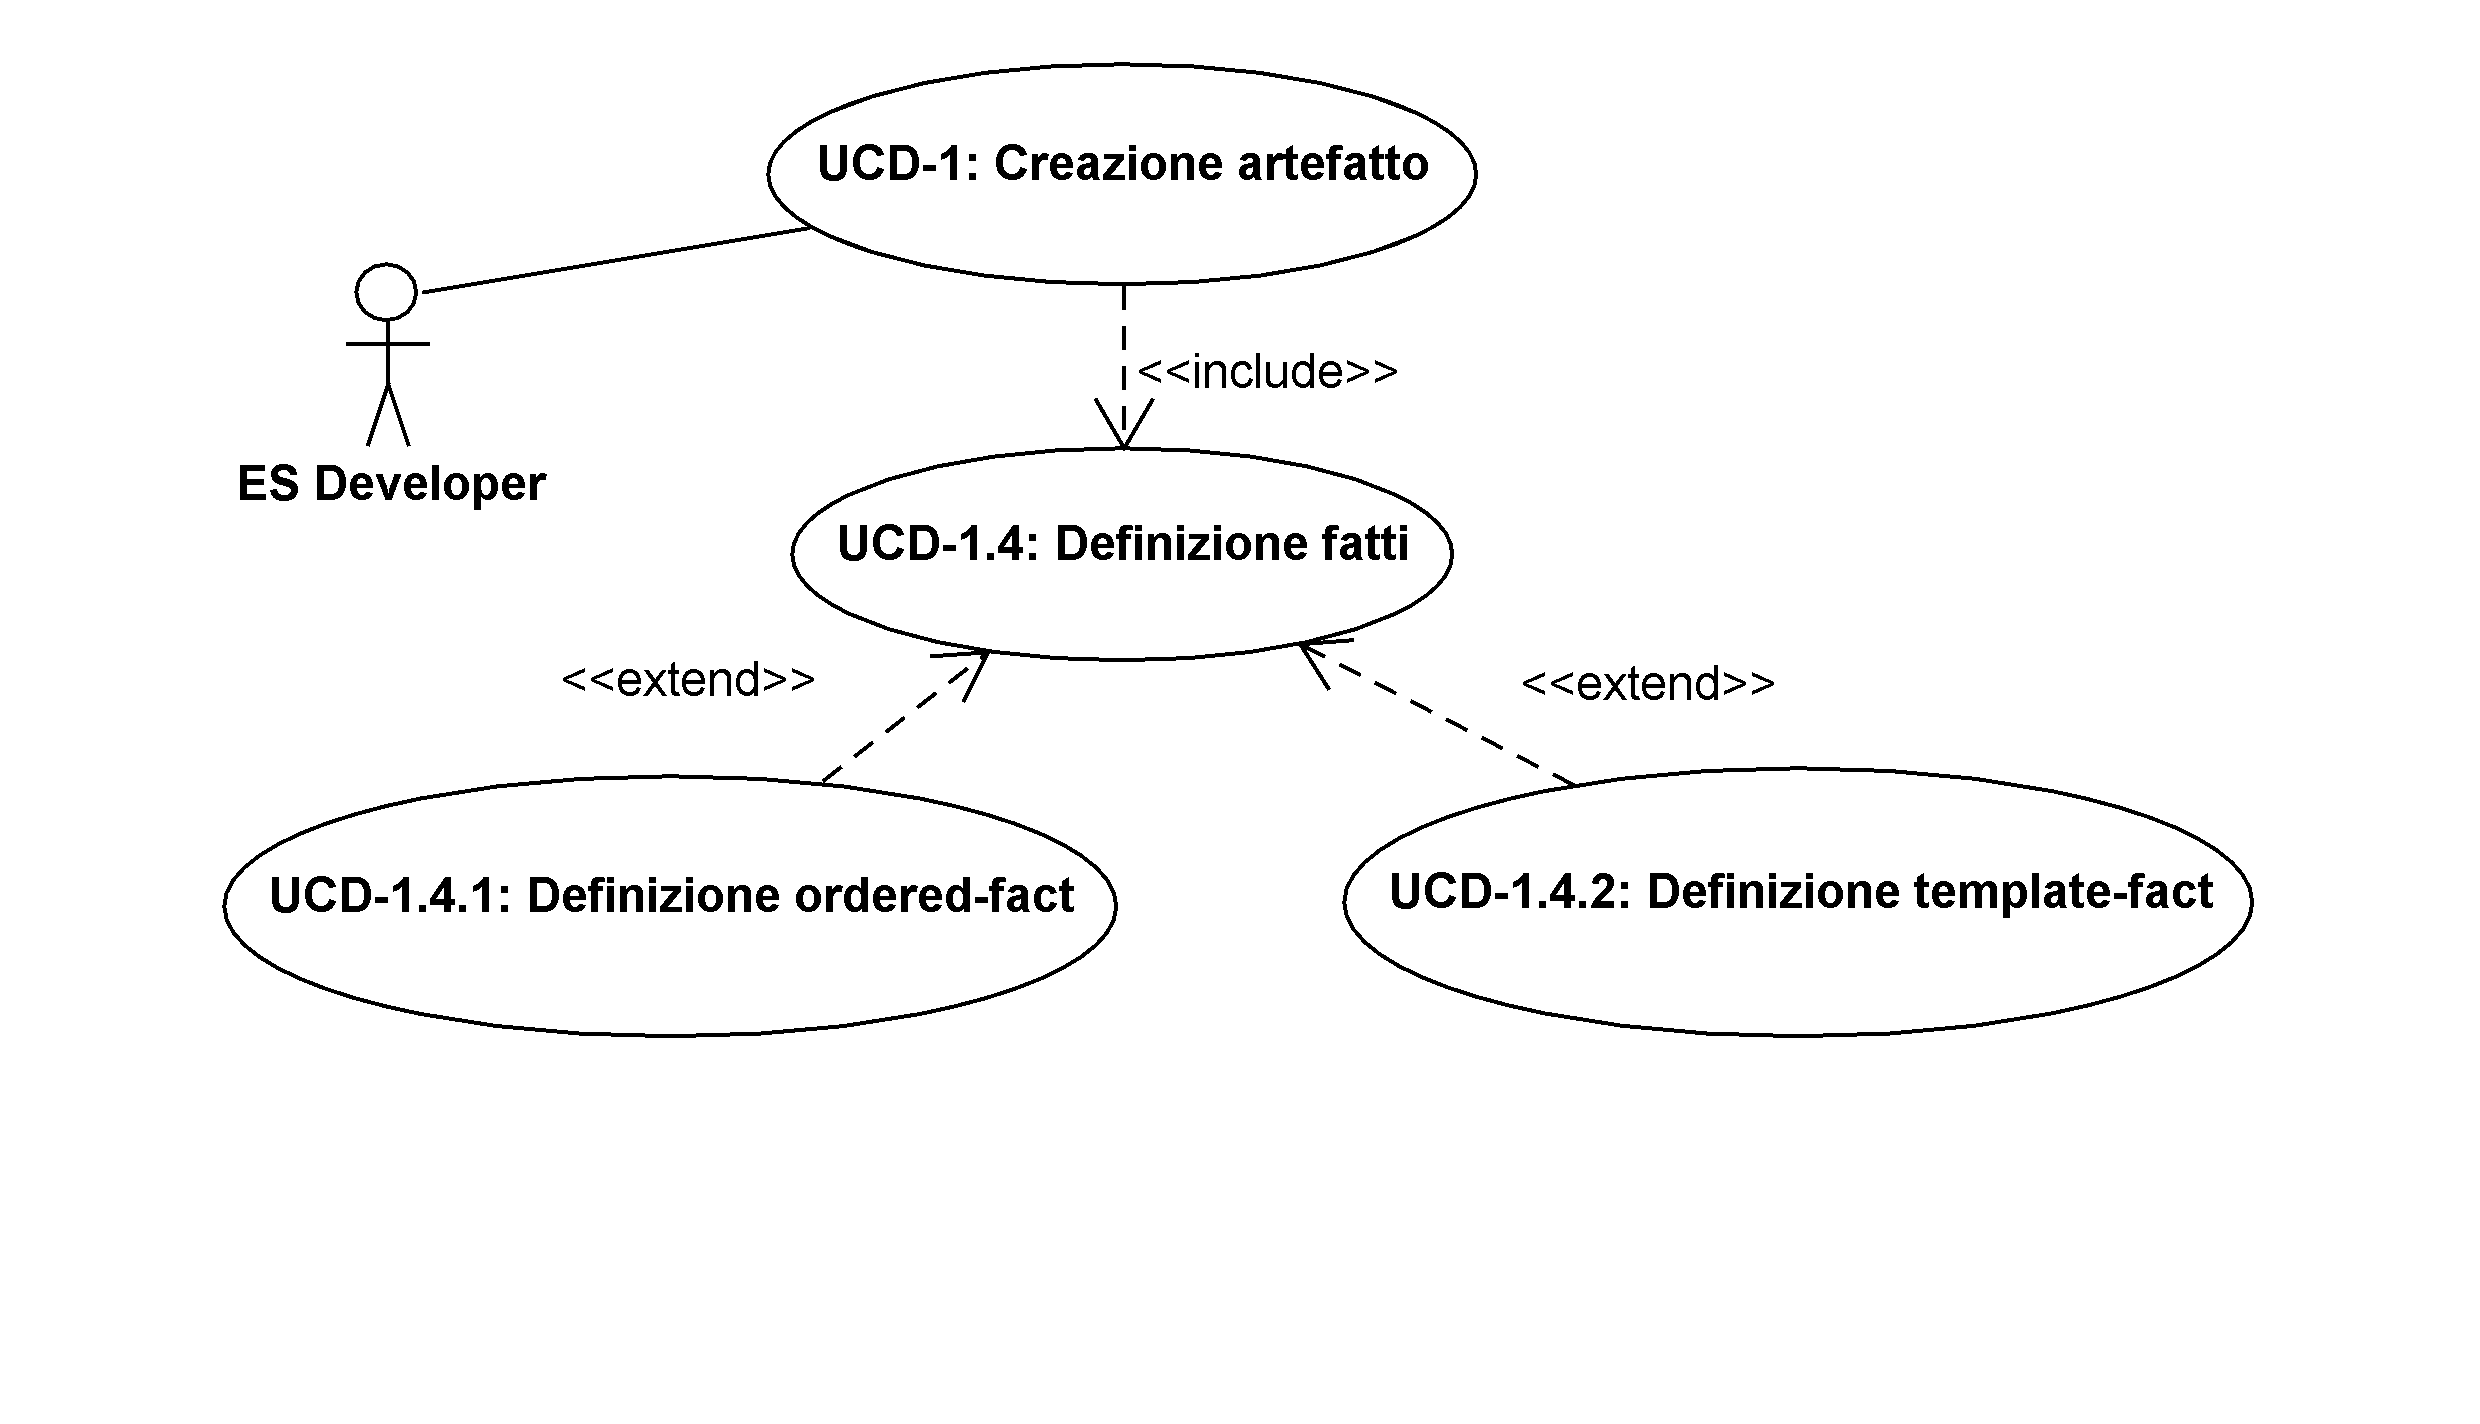
\includegraphics[width=1.1\textwidth]{Immagini/Capitolo2/UseCases/UCD-1_4.png}
\caption{Diagramma dei casi d'uso UCD-1.4}\label{fig:uc-ucd-1.4}
\end{figure}

\begin{itemize}
	\item \textbf{Attori:} ES Developer
	\item \textbf{Scopo e descrizione:} l'ES Developer deve essere in grado di definire un gruppo di fatti iniziali tramite un linguaggio di specifica fornito dal sistema
	\item \textbf{Pre-condizioni:} il software fornisce almeno un linguaggio di specifica
	\item \textbf{Post-condizioni:} la definizione del gruppo di fatti è stata aggiunta ad un artefatto
	\item \textbf{Flusso principale degli eventi:}
		\begin{enumerate}
			\item l'ES Developer definisce un gruppo di fatti specificando il nome
			\item l'ES Developer definisce una serie di fatti da associare al gruppo (si vedano i casi d'uso \emph{UCD-1.4.1} e \emph{UCD-1.4.2})
		\end{enumerate}
	\item \textbf{Flusso alternativo:}
		\begin{enumerate}
			\item se l'ES Developer ha definito precedentemente un modulo, l'ES Developer può definire il gruppo di fatti come componente del modulo.
			\item lo scenario prosegue dal punto 2 del flusso principale
		\end{enumerate}
\end{itemize}

\subparagraph{UCD-1.4.1: Definizione ordered-fact} % nome del caso d'uso SottoGruppo

\begin{itemize}
	\item \textbf{Attori:} ES Developer
	\item \textbf{Scopo e descrizione:}  l'ES Developer deve essere in grado di definire un fatto in notazione \emph{ordered-fact} tramite un linguaggio di specifica fornito dal sistema
	\item \textbf{Pre-condizioni:} il software fornisce almeno un linguaggio di specifica, l'ES Developer ha definito un gruppo di fatti iniziali
	\item \textbf{Post-condizioni:} il fatto in notazione \emph{ordered-fact} è aggiunto al gruppo di fatti iniziali
	\item \textbf{Flusso principale degli eventi:}
		\begin{enumerate}
			\item l'ES Developer definisce un gruppo di fatti iniziali
			\item l'ES Developer definisce un fatto in notazione \emph{ordered-fact} specificando l'elenco di componenti in sequenza
				\begin{itemize}
					\item l'ES Developer può specificare una sequenza di componenti di lunghezza arbitraria
					\item l'ES Developer può specificare una sequenza di componenti di tipo non omogeneo
				\end{itemize}
		\end{enumerate}
	\item \textbf{Flusso alternativo:}
		\begin{enumerate}
			\setcounter{enumi}{1}
			\item l'ES Developer definisce un fatto in notazione \emph{ordered-fact} con componenti identiche a quelle di un fatto specificato in precedenza
			\item il sistema ignora la definizione
		\end{enumerate}
\end{itemize}


\subparagraph{UCD-1.4.2: Definizione template-fact} % nome del caso d'uso SottoGruppo

\begin{itemize}
	\item \textbf{Attori:} ES Developer
	\item \textbf{Scopo e descrizione:}  l'ES Developer deve essere in grado di definire un fatto in notazione \emph{template-fact} tramite un linguaggio di specifica fornito dal sistema
	\item \textbf{Pre-condizioni:} il software fornisce almeno un linguaggio di specifica, l'ES Developer ha definito un gruppo di fatti iniziali
	\item \textbf{Post-condizioni:} il fatto in notazione \emph{template-fact} è aggiunto al gruppo di fatti iniziali
	\item \textbf{Flusso principale degli eventi:}
		\begin{enumerate}
			\item l'ES Developer definisce un gruppo di fatti iniziali
			\item l'ES Developer definisce un fatto in notazione \emph{template-fact} specificando il nome del \emph{template} di riferimento
			\item l'ES Developer definisce i valori degli slot (risp. multi-slot)
				\begin{itemize}
					\item l'ES Developer può specificare una sequenza di componenti di lunghezza arbitraria per i \emph{multi-slot}
					\item l'ES Developer può specificare un elemento per gli \emph{slot}
				\end{itemize}
			\item il sistema completa la definizione del fatto associando i valori di default agli \emph{slot} (risp. \emph{multi-slot}) non definiti.
		\end{enumerate}
	\item \textbf{Flusso alternativo \#1:}
		\begin{enumerate}
			\setcounter{enumi}{1}
			\item l'ES Developer fornisce un nome di template non valido
			\item il sistema rifiuta la definizione e notifica l'errore
			\item il sistema torna allo stato iniziale
		\end{enumerate}
	\item \textbf{Flusso alternativo \#2:}
		\begin{enumerate}
			\setcounter{enumi}{2}
			\item l'ES Developer assegna un valore ad uno \emph{slot} (risp. \emph{multi-slot}) non definito nella definizione del \emph{template}.
			\item il sistema rifiuta la definizione e notifica l'errore
			\item il sistema torna allo stato iniziale
		\end{enumerate}
\end{itemize}


\paragraph{UCD-1.5: Definizione variabile globale} % nome del caso d'uso Gruppo

\begin{itemize}
	\item \textbf{Attori:} ES Developer
	\item \textbf{Scopo e descrizione:}  l'ES Developer deve essere in grado di definire una variabile globale tramite un linguaggio di specifica.
	\item \textbf{Pre-condizioni:} il software fornisce almeno un linguaggio di specifica
	\item \textbf{Post-condizioni:} la definizione della variabile globale è stata aggiunta ad un artefatto
	\item \textbf{Flusso principale degli eventi:}
		\begin{enumerate}
			\item l'ES Developer definisce una variabile globale, indicando nome e valore iniziale
			\item il sistema valuta la definizione
		\end{enumerate}
	\item \textbf{Flusso alternativo \#1:} 
		\begin{enumerate}
			\setcounter{enumi}{1}
			\item se l'ES Developer ha indicato come nome per la variabile globale uno già utilizzato, il valore iniziale fornito viene sostituito a quello della definizione precedente
			\item lo scenario prosegue dal punto 2 del flusso principale
		\end{enumerate}
	\item \textbf{Flusso alternativo \#2:} 
		\begin{enumerate}
			\item se l'ES Developer ha definito precedentemente un modulo, l'ES Developer può definire la variabile globale come componente del modulo.
			\item lo scenario prosegue dal punto 2 del flusso principale
		\end{enumerate}
\end{itemize}

\paragraph{UCD-1.6: Definizione funzione} % nome del caso d'uso Gruppo

\begin{itemize}
	\item \textbf{Attori:} ES Developer
	\item \textbf{Scopo e descrizione:} l'ES Developer deve essere in grado di definire una funzione tramite un linguaggio di specifica
	\item \textbf{Pre-condizioni:} il software fornisce almeno un linguaggio di specifica
	\item \textbf{Post-condizioni:} la definizione della funzione è stata aggiunta ad un artefatto
	\item \textbf{Flusso principale degli eventi:}
		\begin{enumerate}
			\item l'ES Developer definisce una funzione utente, indicando nome, parametri e corpo della funzione
			\item il sistema valuta il nome della funzione
		\end{enumerate}
	\item \textbf{Flusso alternativo \#1:}
		\begin{enumerate}
			\setcounter{enumi}{1}
			\item se il nome fornito dall'ES Developer è già utilizzato da una definizione di funzione (di sistema o utente), il sistema rifiuta la definizione e notifica l'errore
			\item il sistema ritorna allo stato iniziale
		\end{enumerate}
	\item \textbf{Flusso alternativo \#2:}
		\begin{enumerate}
			\item se l'ES Developer ha definito precedentemente un modulo, l'ES Developer può definire la funzione utente come componente del modulo
			\item lo scenario procede dal punto 2 del flusso principale
		\end{enumerate}
\end{itemize}

\pagebreak

\subsubsection{UCD-2: Testa artefatto}

%UCD-2: Testa artefatto

\begin{figure}
\centering
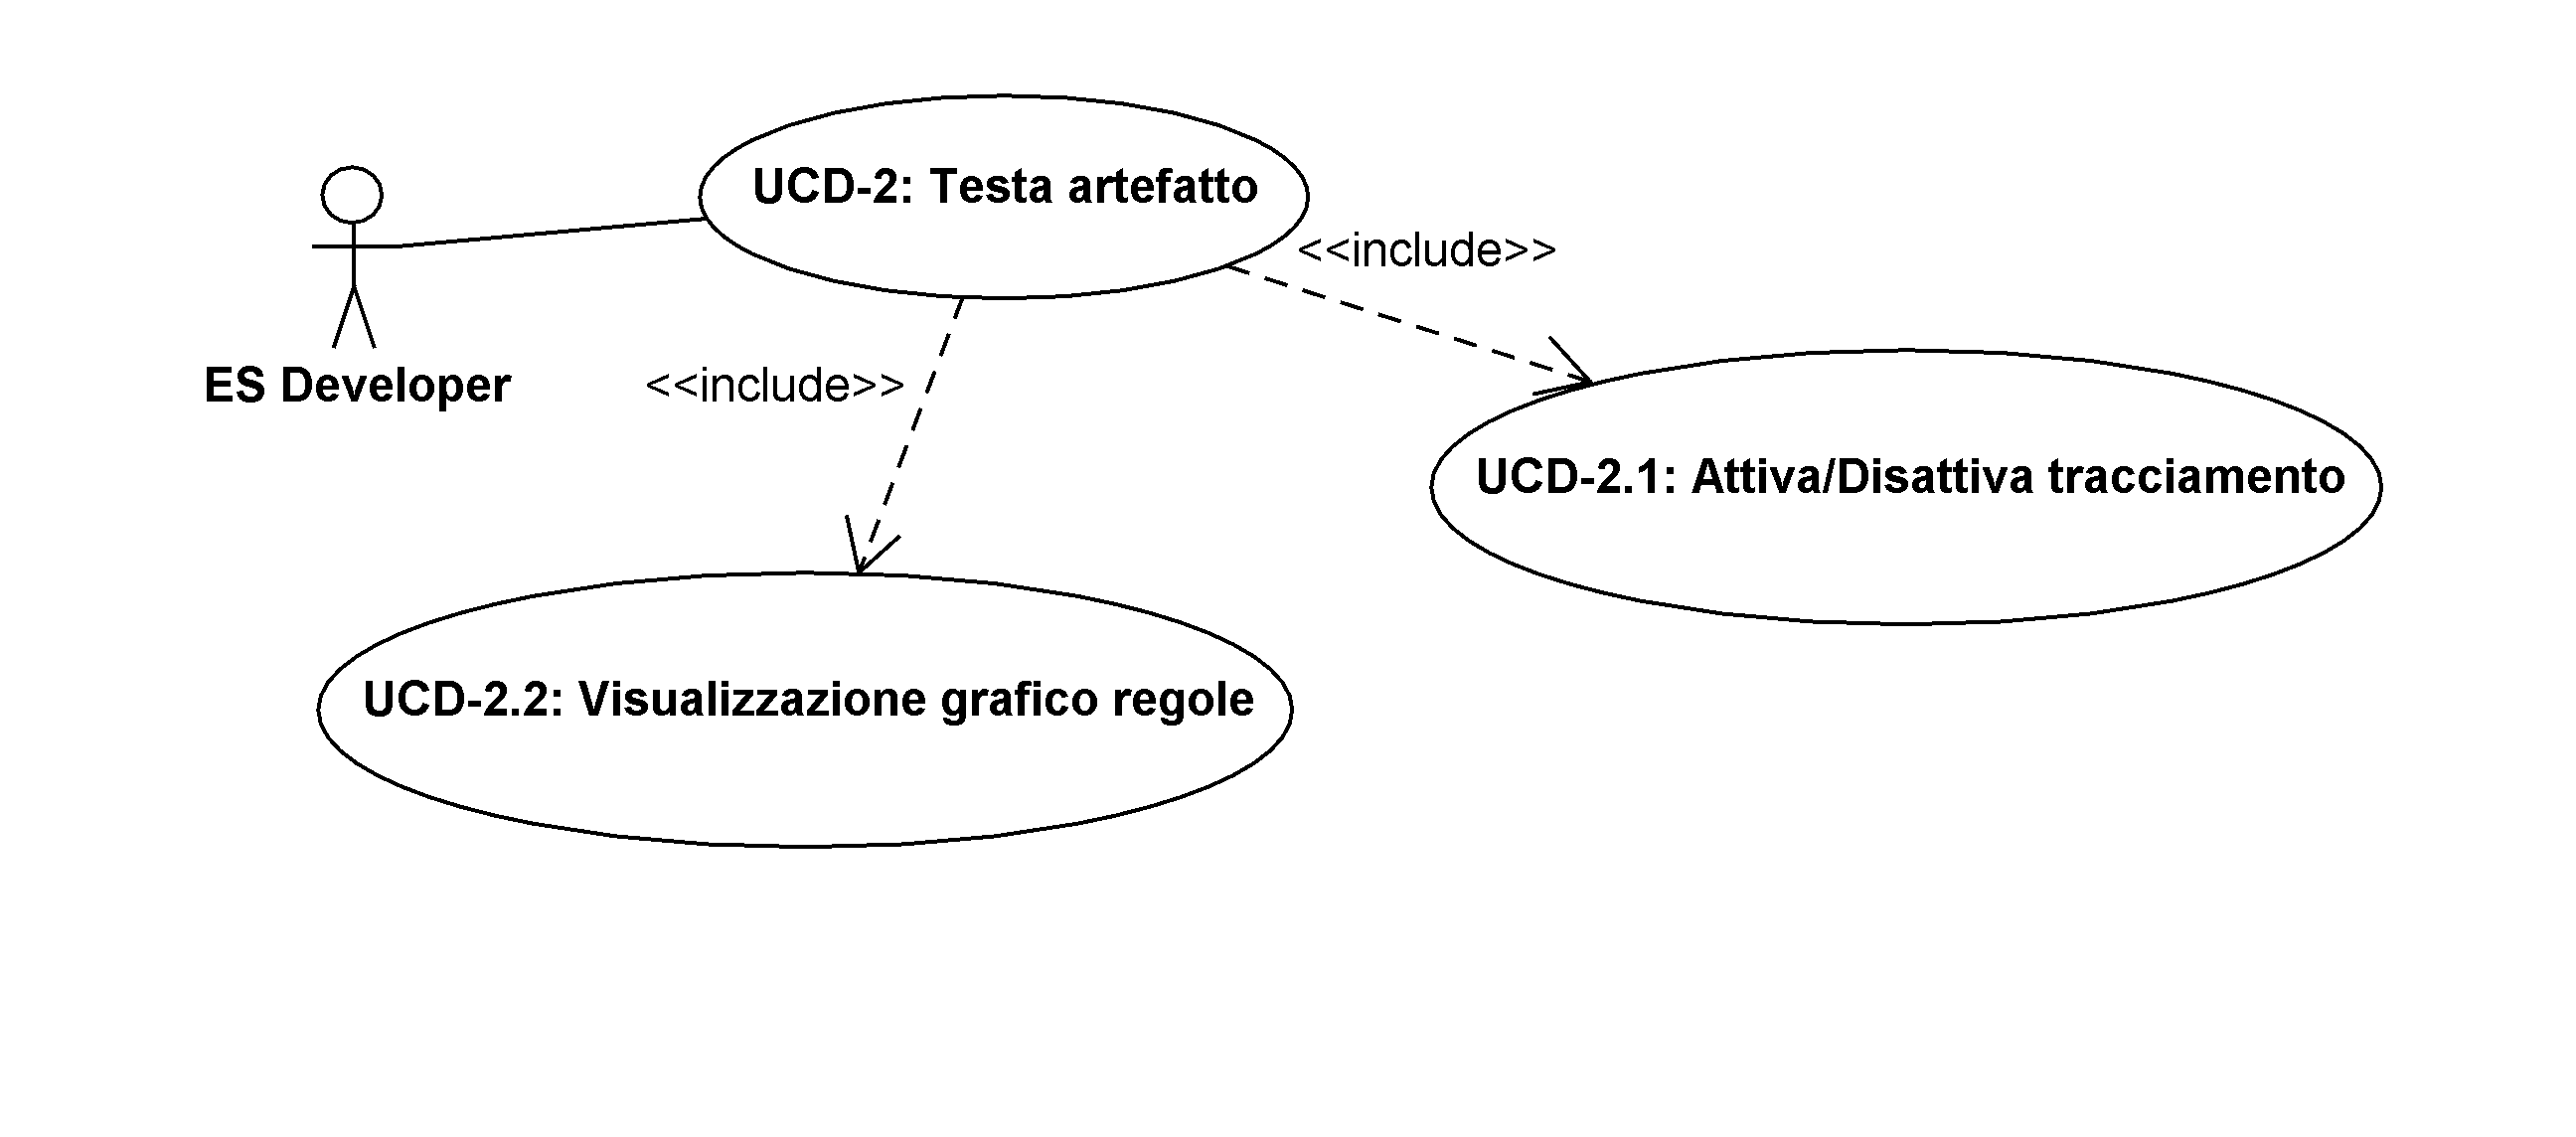
\includegraphics[width=1.1\textwidth]{Immagini/Capitolo2/UseCases/UCD-2.png}
\caption{Diagramma dei casi d'uso UCD-2}\label{fig:uc-ucd-2}
\end{figure}


\begin{itemize}
	\item \textbf{Attori:} ES Developer
	\item \textbf{Scopo e descrizione:} un ES Developer deve essere in grado di testare l'artefatto prodotto valutando un registro del funzionamento dello stesso e le modalità con le quali le definizioni appartenenti all'artefatto vengono interpretate.
	\item \textbf{Pre-condizioni:} l'ES Developer ha realizzato un artefatto, l'artefatto è stato caricato nel sistema. Il sistema attende istruzioni
	\item \textbf{Post-condizioni:} il funzionamento dell'artefatto è stato valutato
	\item \textbf{Flusso principale degli eventi:}
		\begin{enumerate}
			\item l'ES Developer richiede al sistema informazioni per valutare l'artefatto.
			\begin{itemize}
				\item l'ES Developer può richiedere informazioni sull'attività del sistema (si veda caso d'uso \emph{UCD-2.1})
				\item l'ES Developer può richiedere informazioni su come l'artefatto viene interpretato (si veda caso d'uso \emph{UCD-2.2}).
			\end{itemize}
			\item il sistema fornisce le informazioni richieste.
		\end{enumerate}
\end{itemize}


\paragraph{UCD-2.1: Attiva/Disattiva tracciamento}

\begin{figure}
\centering
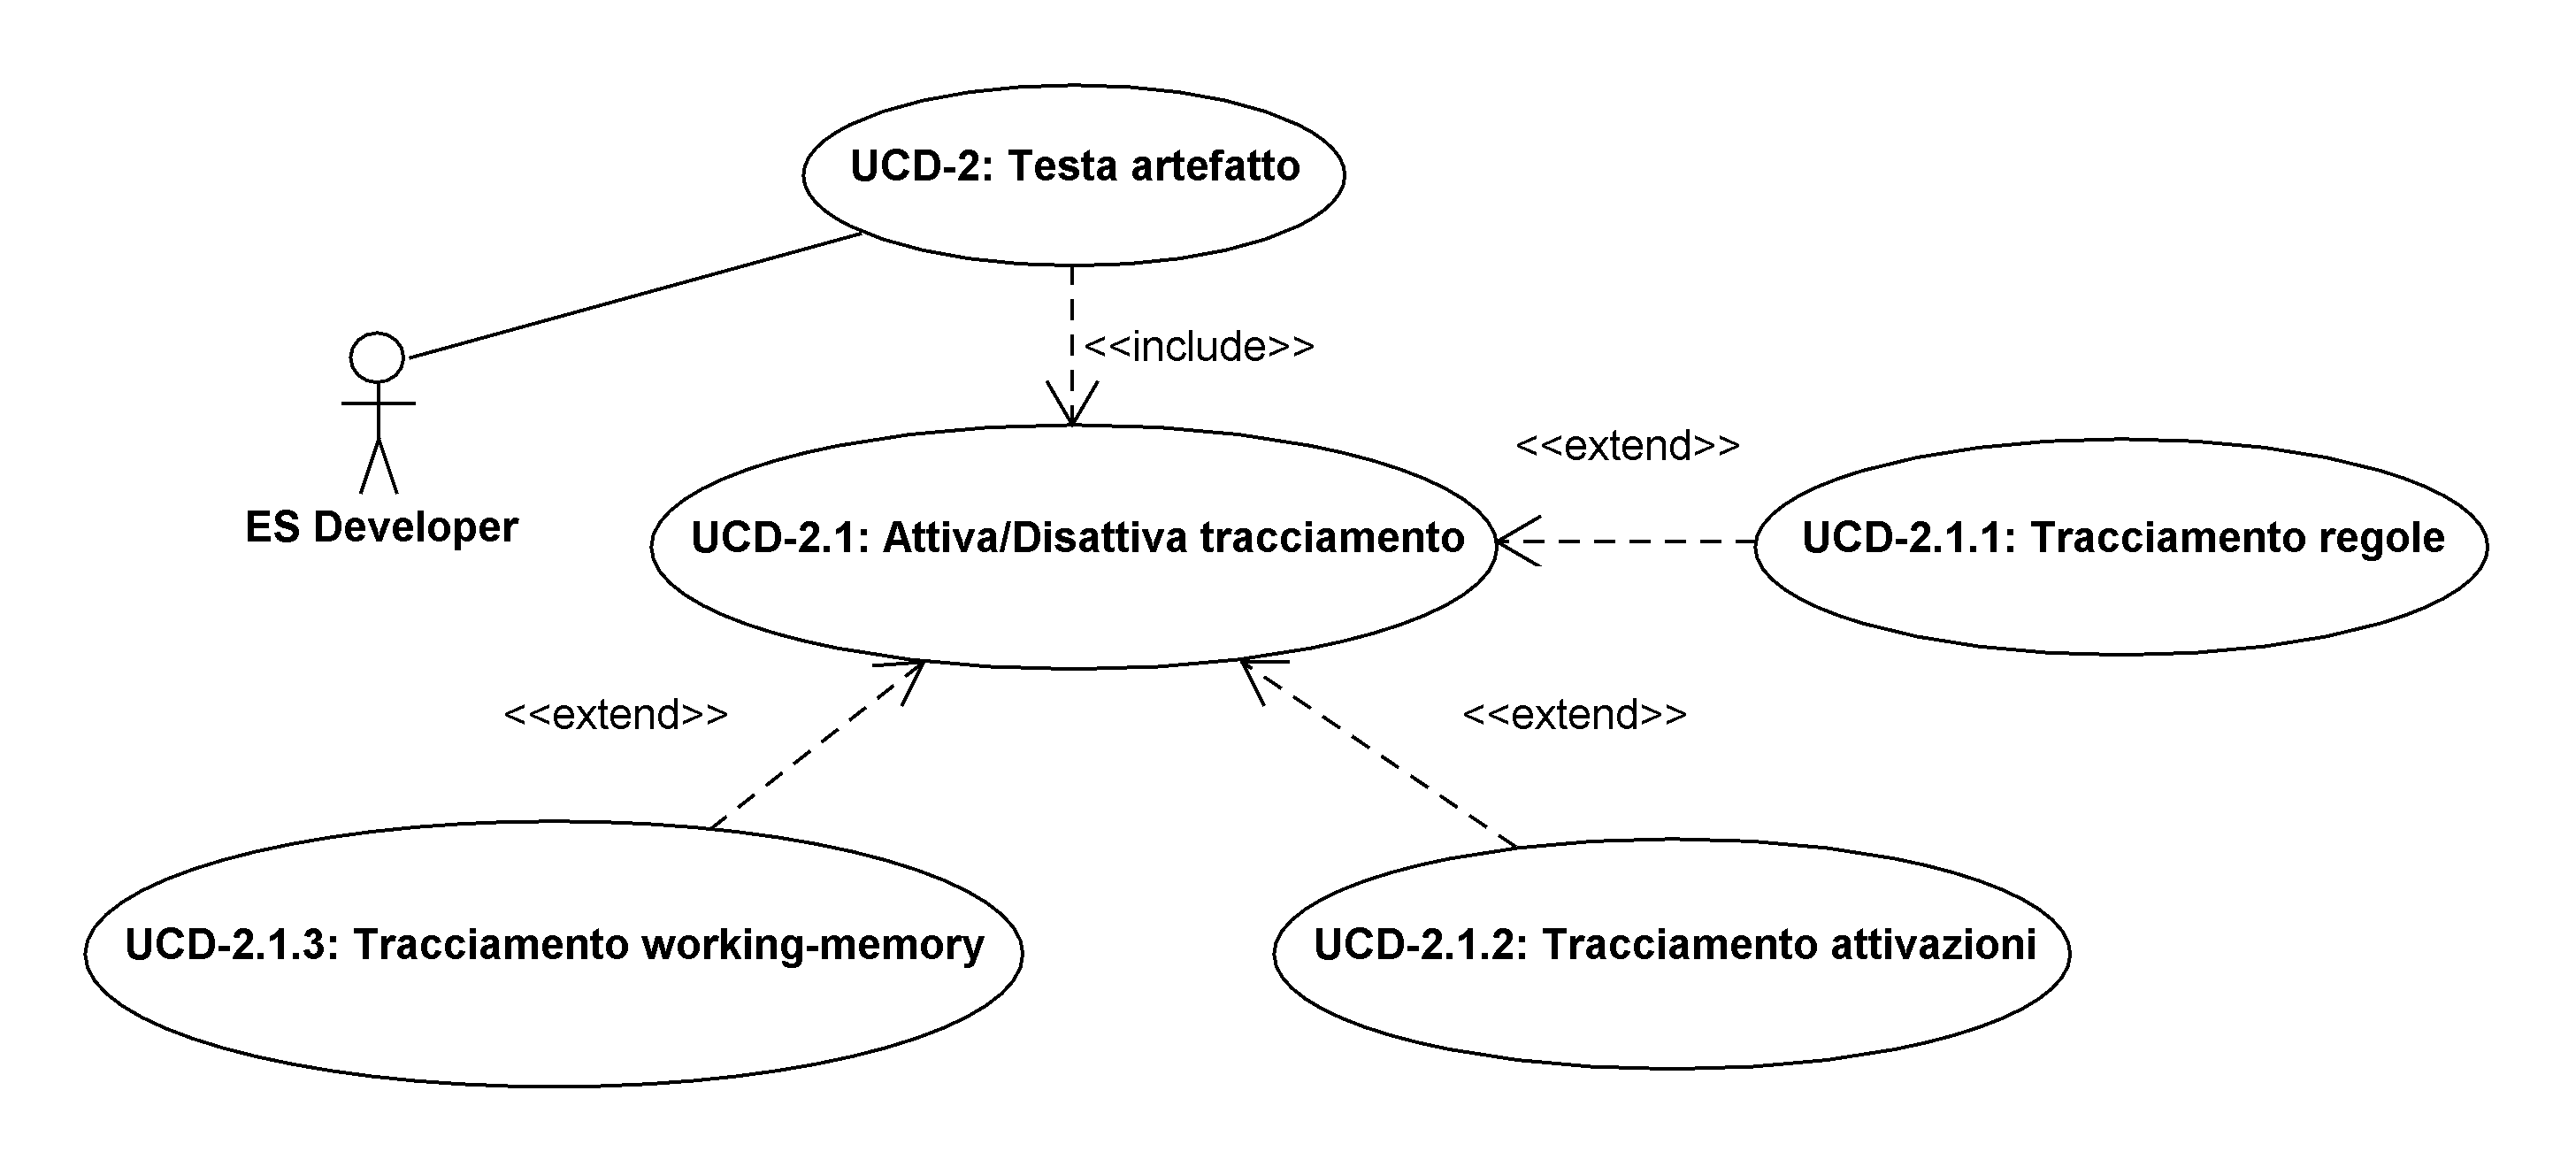
\includegraphics[width=1.1\textwidth]{Immagini/Capitolo2/UseCases/UCD-2_1.png}
\caption{Diagramma dei casi d'uso UCD-2.1}\label{fig:uc-ucd-2.1}
\end{figure}

La descrizione comprende quella dei casi d'uso \emph{UCD-2.1.1}, \emph{UCD-2.1.2}, \emph{UCD-2.1.3} in quanto identici, a meno del tipo di informazioni che vengono tracciate.

\begin{itemize}
	\item \textbf{Attori:} ES Developer
	\item \textbf{Scopo e descrizione:} un ES Developer deve essere in grado di modificare le impostazioni riguardo al tracciamento di regole, attivazioni e modifiche alla \emph{working-memory}.
	\item \textbf{Pre-condizioni:} ES Developer ha caricato un artefatto nel sistema. Il sistema attende istruzioni
	\item \textbf{Post-condizioni:} le impostazioni di tracciamento risultano modificate
	\item \textbf{Flusso principale degli eventi:}
		\begin{enumerate}
			\item l'ES Developer modifica le impostazioni riguardanti il tracciamento
			\begin{itemize}
				\item l'ES Developer può attivare (risp. disattivare) il tracciamento delle regole eseguite
				\item l'ES Developer può attivare (risp. disattivare) il tracciamento delle attivazioni disponibili
				\item l'ES Developer può attivare (risp. disattivare) il tracciamento delle modifiche alla \emph{working-memory}				
			\end{itemize}
			\item il sistema modifica le impostazioni di tracciamento dell'elemento indicato
		\end{enumerate}
	\item \textbf{Flusso alternativo:}
		\begin{enumerate}
			\item l'ES Developer richiede l'attivazione (risp. disattivazione) di un tracciamento già attivo (risp. non attivo).
			\item il sistema ignora la richiesta
		\end{enumerate}
\end{itemize}


\paragraph{UCD-2.2: Visualizzazione grafico regole}

\begin{itemize}
	\item \textbf{Attori:} ES Developer
	\item \textbf{Scopo e descrizione:} un ES Developer deve essere in grado di richiedere informazioni riguardanti le modalità con le quali il sistema interpreta una regola.
	\item \textbf{Pre-condizioni:} ES Developer ha caricato un artefatto nel sistema. Il sistema attende istruzioni
	\item \textbf{Post-condizioni:} Il sistema attende istruzioni
	\item \textbf{Flusso principale degli eventi:}
		\begin{enumerate}
			\item l'ES Developer richiede informazioni riguardanti l'interpretazione di una regola
			\begin{itemize}
				\item l'ES Developer può indicare una regola specificandone il nome
				\item l'ES Developer può indicare un insieme di regole specificandone i nomi
			\end{itemize}
			\item il sistema fornisce le informazioni richieste
		\end{enumerate}
	\item \textbf{Flusso alternativo \#1:}
		\begin{enumerate}
			\item l'ES Developer specifica un nome di regola non valido
			\item il sistema ignora la richiesta, notificando l'errore
		\end{enumerate}
	\item \textbf{Flusso alternativo \#2:}
		\begin{enumerate}
			\item l'ES Developer inserisce un nome non valido specificando un insieme di regole
			\item il sistema ignora la richiesta, notificando l'errore
		\end{enumerate}
\end{itemize}

\pagebreak

\subsubsection{UCE-1: Modifica funzioni di sistema}

%UCE-1: Modifica funzioni di sistema

Nel proseguo dei paragrafi relativi ai casi d'uso \emph{UCE}, il nome dell'attore \emph{Environment Developer} verrà abbreviato con la sigla \emph{ED}.

\begin{figure}
\centering
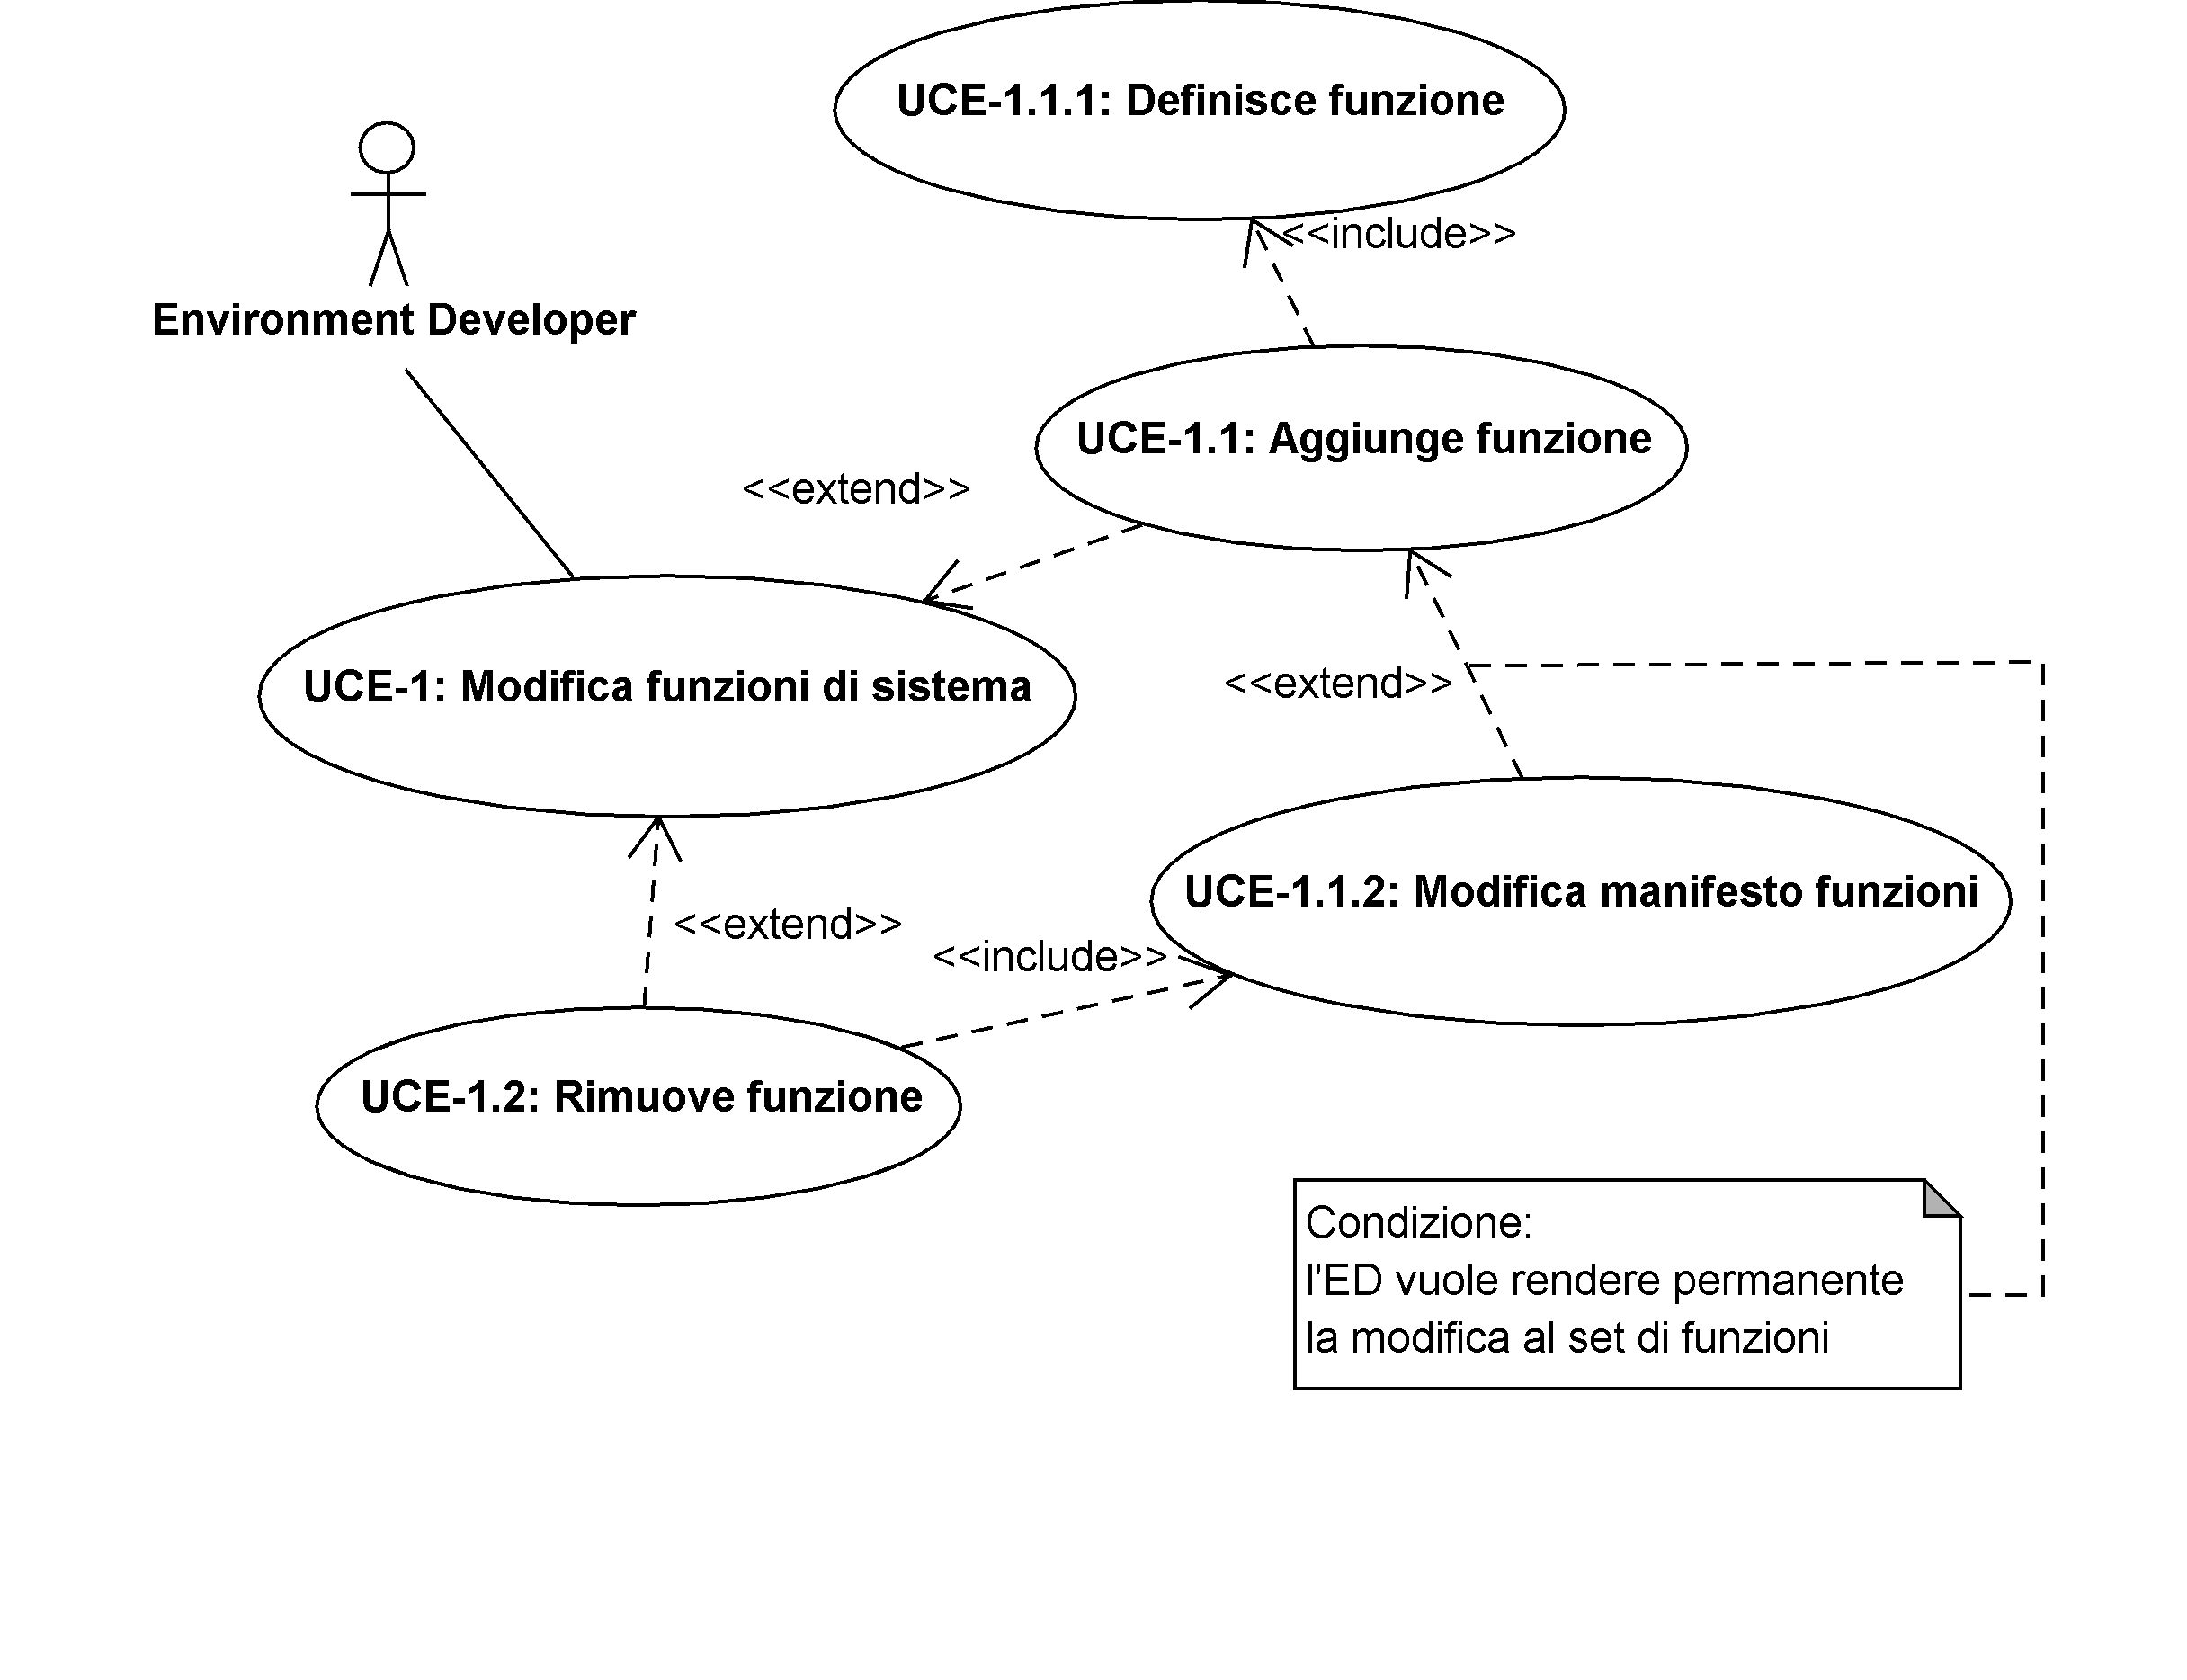
\includegraphics[width=1.1\textwidth]{Immagini/Capitolo2/UseCases/UCE-1.png}
\caption{Diagramma dei casi d'uso UCE-1}\label{fig:uc-uce-1}
\end{figure}


\begin{itemize}
	\item \textbf{Attori:} Environment Developer (\emph{ED})
	\item \textbf{Scopo e descrizione:} l'ED deve essere in grado di modificare il set di funzioni di sistema incluse nel software
	\item \textbf{Pre-condizioni:} il software fornisce meccanismi per estendere il set di funzioni di sistema
	\item \textbf{Post-condizioni:} il set di funzioni di sistema risulta modificato
	\item \textbf{Flusso principale degli eventi:}
		\begin{enumerate}
			\item l'ED esegue una modifica al set di funzioni di sistema.
			\begin{itemize}
				\item l'ED può rimuovere la definizione di una funzione esistente (si veda caso d'uso \emph{UCE-1.2})
				\item l'ED può aggiungere una nuova definizione di funzione di sistema (si veda caso d'uso \emph{UCE-1.1}).
			\end{itemize}
			\item il sistema carica il set modificato di funzioni sistema.
		\end{enumerate}
\end{itemize}


\paragraph{UCE-1.1: Aggiunge funzione}

La descrizione comprende quella del caso d'uso \emph{UCE-1.1.1}

\begin{itemize}
	\item \textbf{Attori:} ED
	\item \textbf{Scopo e descrizione:} un ED deve essere in grado di aggiungere una nuova funzione al set di funzioni di sistema.
	\item \textbf{Pre-condizioni:} il sistema è stato configurato correttamente. Il sistema non è attivo
	\item \textbf{Post-condizioni:} il sistema è attivo e una nuova funzione è disponibile nel set di funzioni di sistema
	\item \textbf{Flusso principale degli eventi:}
		\begin{enumerate}
			\item l'ED definisce il corpo di una nuova funzione di sistema (\emph{UCE-1.1.1})
			\item l'ED definisce la firma di una nuova funzione di sistema
				\begin{itemize}
					\item l'ED specifica un nome di funzione
					\item l'ED specifica un numero di parametri accettati (minimi, massimi, esatti)
					\item l'ED specifica il tipo dei parametri accettati
					\item l'ED specifica il tipo dei risultati
				\end{itemize}
			\item l'ED avvia il software
			\item l'ED richiede al software il caricamento della nuova funzione
				\begin{itemize}
					\item l'ED indica il file contenente il corpo della funzione
					\item l'ED indica la posizione della firma della funzione
				\end{itemize}
			\item la richiesta è valutata dal sistema
			\item la nuova definizione viene resa disponibile
		\end{enumerate}
	\item \textbf{Flusso alternativo \#1:}
		\begin{enumerate}
			\setcounter{enumi}{4}
			\item se l'ED ha specificato un nome di funzione già utilizzato, il sistema ignora la nuova definizione, notificando l'errore
		\end{enumerate}

	\item \textbf{Flusso alternativo \#2:}
		\begin{enumerate}
			\setcounter{enumi}{1}
			\item l'ED definisce la firma della nuova funzione indicando solo il nome e il tipo dei risultati della funzione
			\item \emph{analogo al punto 3 del flusso principale}
			\item \emph{analogo al punto 4 del flusso principale}
			\item \emph{analogo al punto 5 del flusso principale}						
			\item la firma viene integrata automaticamente dal sistema in modo che la funzione accetti un numero ed un tipo arbitrario di valori
			\item lo scenario prosegue con il punto 6 del flusso principale
		\end{enumerate}

	
\end{itemize}


\subparagraph{UCE-1.1.2: Modifica manifesto funzioni} % nome del caso d'uso SottoGruppo

\begin{itemize}
	\item \textbf{Attori:} ED
	\item \textbf{Scopo e descrizione:} ED deve essere in grado di apportare una modifica permanente al set di funzioni di sistema modificando un registro contenente l'elenco di funzioni di sistema
	\item \textbf{Pre-condizioni:} l'ED vuole rendere permanente l'aggiunta o la rimozione di una funzione di sistema. Il software non è attivo.
	\item \textbf{Post-condizioni:} il software è attivo, la modifica apportata al registro viene evidenziata nel set di funzioni di sistema disponibili
	\item \textbf{Flusso principale degli eventi:}
		\begin{enumerate}
			\item l'ED modifica il registro contenente l'elenco delle funzioni di sistema
				\begin{itemize}
					\item l'ED può aggiungere una nuova funzione all'elenco specificando il file contenente il corpo e la posizione della firma della funzione
					\item l'ED può rimuovere una funzione eliminandone le informazioni dall'elenco
				\end{itemize}
			\item l'ED salva le modifiche al registro
			\item l'ED avvia il sistema
			\item le modifiche vengono valutate dal sistema
			\item il set di funzioni disponibili viene modificato
			\item l'inizializzazione del software prosegue
		\end{enumerate}
	\item \textbf{Flusso alternativo:} 
		\begin{enumerate}
			\setcounter{enumi}{4}
			\item se l'ED ha apportato modifiche non valide al registro delle funzioni di sistema, il software notifica l'errore
			\item l'inizializzazione del software viene arrestata
		\end{enumerate}
\end{itemize}


\paragraph{UCE-1.2: Rimuove funzione}

\begin{itemize}
	\item \textbf{Attori:} ED
	\item \textbf{Scopo e descrizione:} ED deve essere in grado di rimuovere una funzione di sistema da quelle disponibili.
	\item \textbf{Pre-condizioni:} il software è configurato correttamente, il software non è attivo.
	\item \textbf{Post-condizioni:} Il software è attivo, la funzione di sistema non è presente fra quelle disponibili
	\item \textbf{Flusso principale degli eventi:}
		\begin{enumerate}
			\item l'ED modifica il manifesto delle funzioni di sistema rimuovendo le informazioni riguardanti la funzione (si guardi caso il d'uso \emph{UCE-1.1.2})
		\end{enumerate}
\end{itemize}

\pagebreak

\subsubsection{UCE-2: Monitorizza evento}

%UCE-2: Monitorizza evento

\begin{figure}
\centering
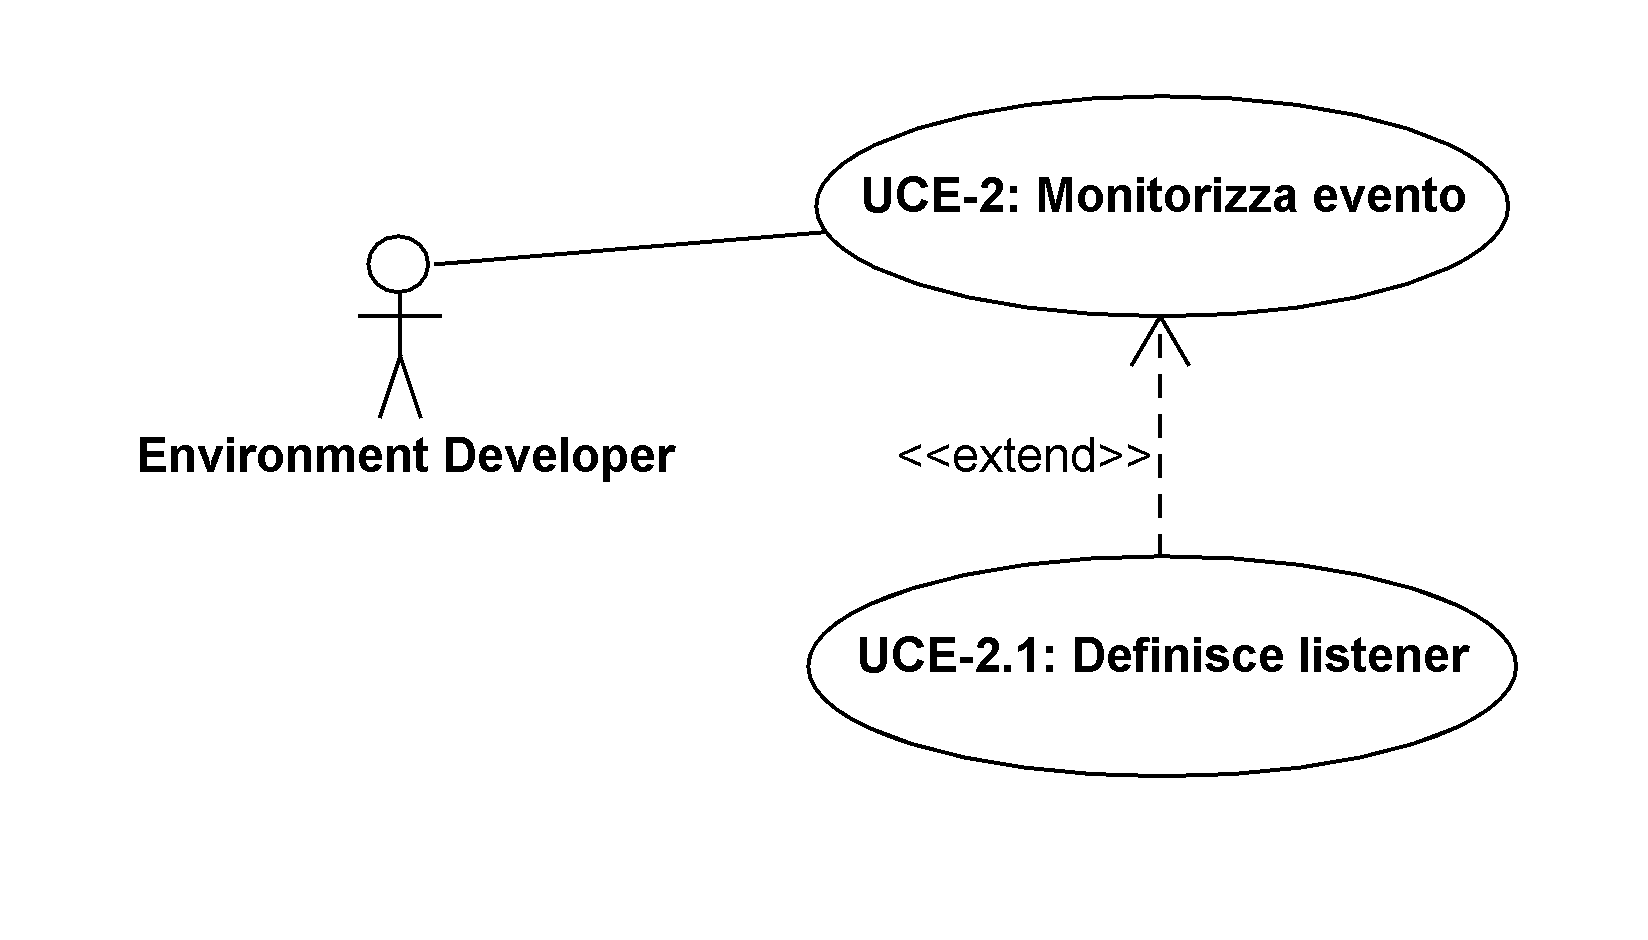
\includegraphics[width=1.1\textwidth]{Immagini/Capitolo2/UseCases/UCE-2.png}
\caption{Diagramma dei casi d'uso UCE-2}\label{fig:uc-uce-2}
\end{figure}


\begin{itemize}
	\item \textbf{Attori:} ED
	\item \textbf{Scopo e descrizione:} l'ED deve essere in grado di specificare un nuovo evento e definire un comportamento da associare al verificarsi dell'evento
	\item \textbf{Pre-condizioni:} il software fornisce meccanismi per la definizione e la notifica di un evento
	\item \textbf{Post-condizioni:} il comportamento specificato dall'ED viene eseguito al verificarsi dell'evento atteso
	\item \textbf{Flusso principale degli eventi:}
		\begin{enumerate}
			\item l'ED specifica un nuovo evento
			\item l'ED specifica un \emph{listener} che realizzi un comportamento al verificarsi di un evento (si guardi il caso d'uso \emph{UCE-2.1})
			\item l'ED avvia il sistema
			\item l'ED avvia un'elaborazione
			\item il verificarsi dell'evento provoca l'esecuzione del comportamento definito
		\end{enumerate}
\end{itemize}


\paragraph{UCE-2.1: Definisce listener}

\begin{itemize}
	\item \textbf{Attori:} ED
	\item \textbf{Scopo e descrizione:} un ED deve essere in grado di specificare un comportamento da eseguire al verificarsi di un evento
	\item \textbf{Pre-condizioni:} il sistema è stato configurato correttamente. Il sistema non è attivo
	\item \textbf{Post-condizioni:} il sistema è attivo e un comportamento è associato all'accadere di un evento
	\item \textbf{Flusso principale degli eventi:}
		\begin{enumerate}
			\item l'ED definisce un comportamento nella forma di un entità \emph{listener}
			\item l'ED registra il \emph{listener} nel sistema
		\end{enumerate}
	
\end{itemize}

\pagebreak

\subsubsection{UCE-3: Aggiunge CRS}

%UCE-3: Aggiunge CRS

\begin{figure}
\centering
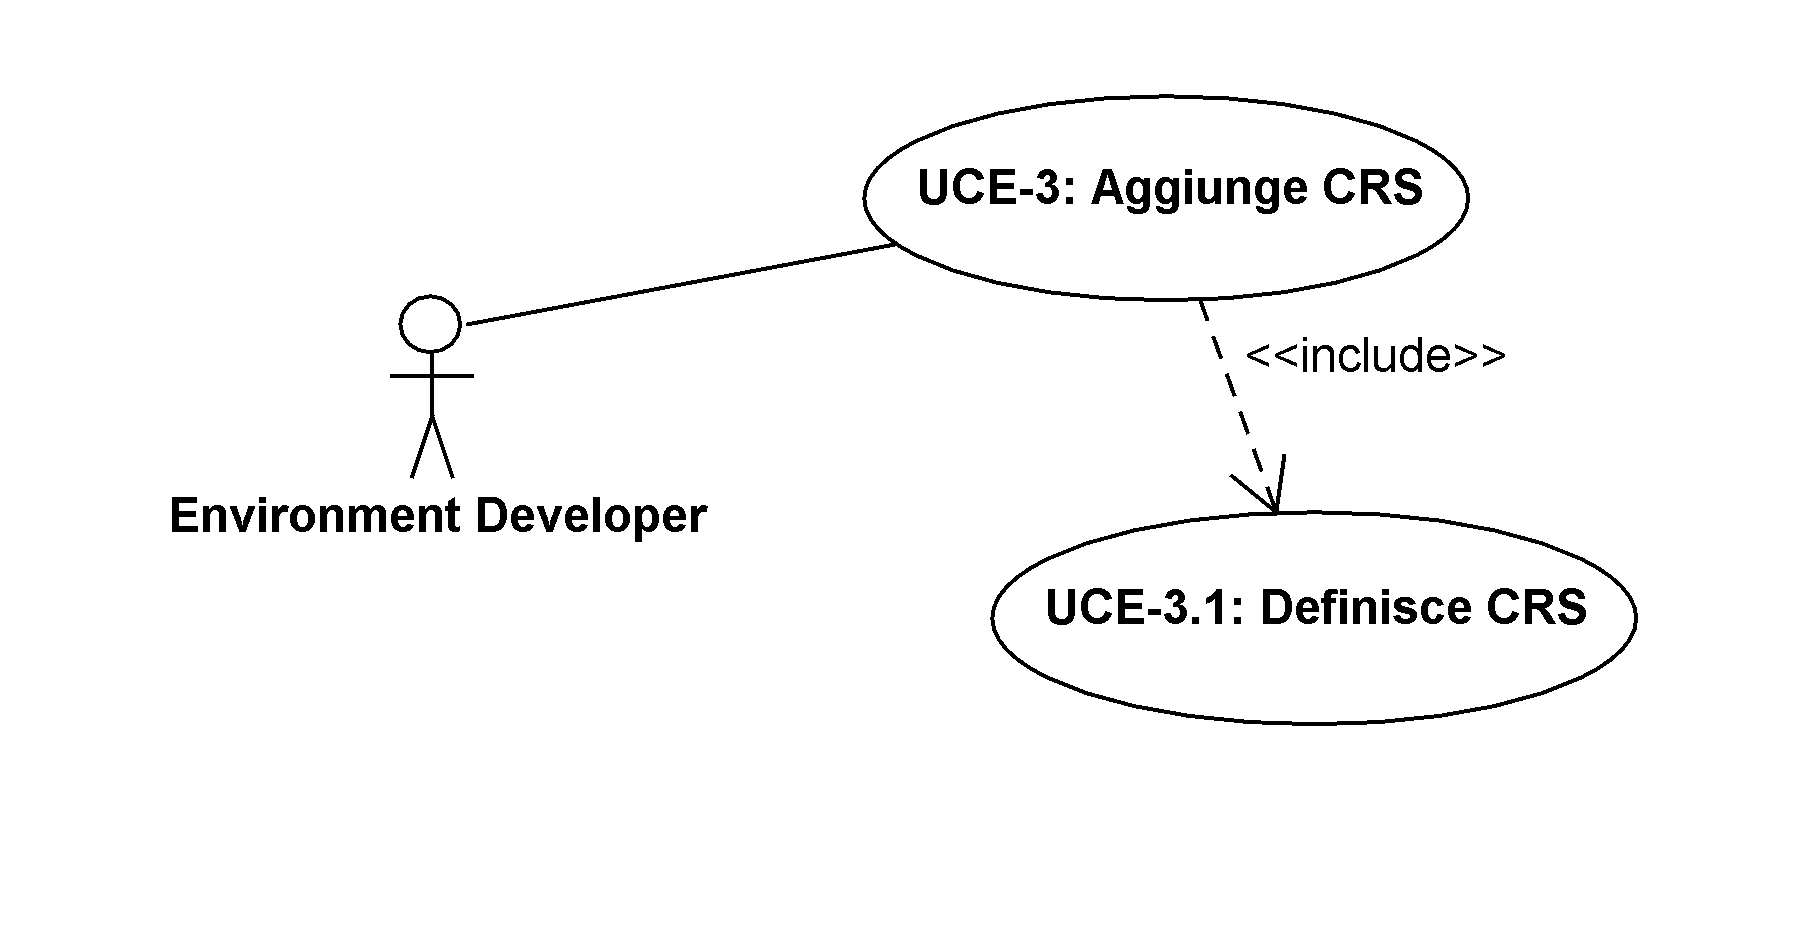
\includegraphics[width=1.1\textwidth]{Immagini/Capitolo2/UseCases/UCE-3.png}
\caption{Diagramma dei casi d'uso UCE-3}\label{fig:uc-uce-3}
\end{figure}


\begin{itemize}
	\item \textbf{Attori:} ED
	\item \textbf{Scopo e descrizione:} l'ED deve essere in grado di definire ed aggiungere una nuova \emph{strategia di risoluzione dei conflitti} (CRS)
	\item \textbf{Pre-condizioni:} il software fornisce meccanismi per la definizione e l'aggiunta di CRS, il sistema non è attivo
	\item \textbf{Post-condizioni:} il sistema è attivo e la una nuova CRS è disponibile
	\item \textbf{Flusso principale degli eventi:}
		\begin{enumerate}
			\item l'ED definisce una nuova CRS attraverso i meccanismi previsti dal sistema (si guardi il caso d'uso \emph{UCE-3.1})
			\item l'ED aggiunge la nuova CRS al sistema
			\item l'ED avvia il sistema
		\end{enumerate}
\end{itemize}


\paragraph{UCE-3.1: Definisce CRS}

\begin{itemize}
	\item \textbf{Attori:} ED
	\item \textbf{Scopo e descrizione:} l'ED deve essere in grado di definire una nuova CRS
	\item \textbf{Pre-condizioni:} il sistema è stato configurato correttamente. Il sistema non è attivo. Il sistema offre meccanismi per la definizione di una nuova CRS.
	\item \textbf{Post-condizioni:} una nuova CRS è disponibile per l'integrazione al sistema
	\item \textbf{Flusso principale degli eventi:}
		\begin{enumerate}
			\item l'ED definisce una nuova CRS
			\item l'ED realizza la CRS in una unità di elaborazione separata e raggiungibile al software
		\end{enumerate}
	
\end{itemize}

\pagebreak

\subsubsection{UCE-4: Testa environment}

%UCE-4: Testa environment

\begin{figure}
\centering
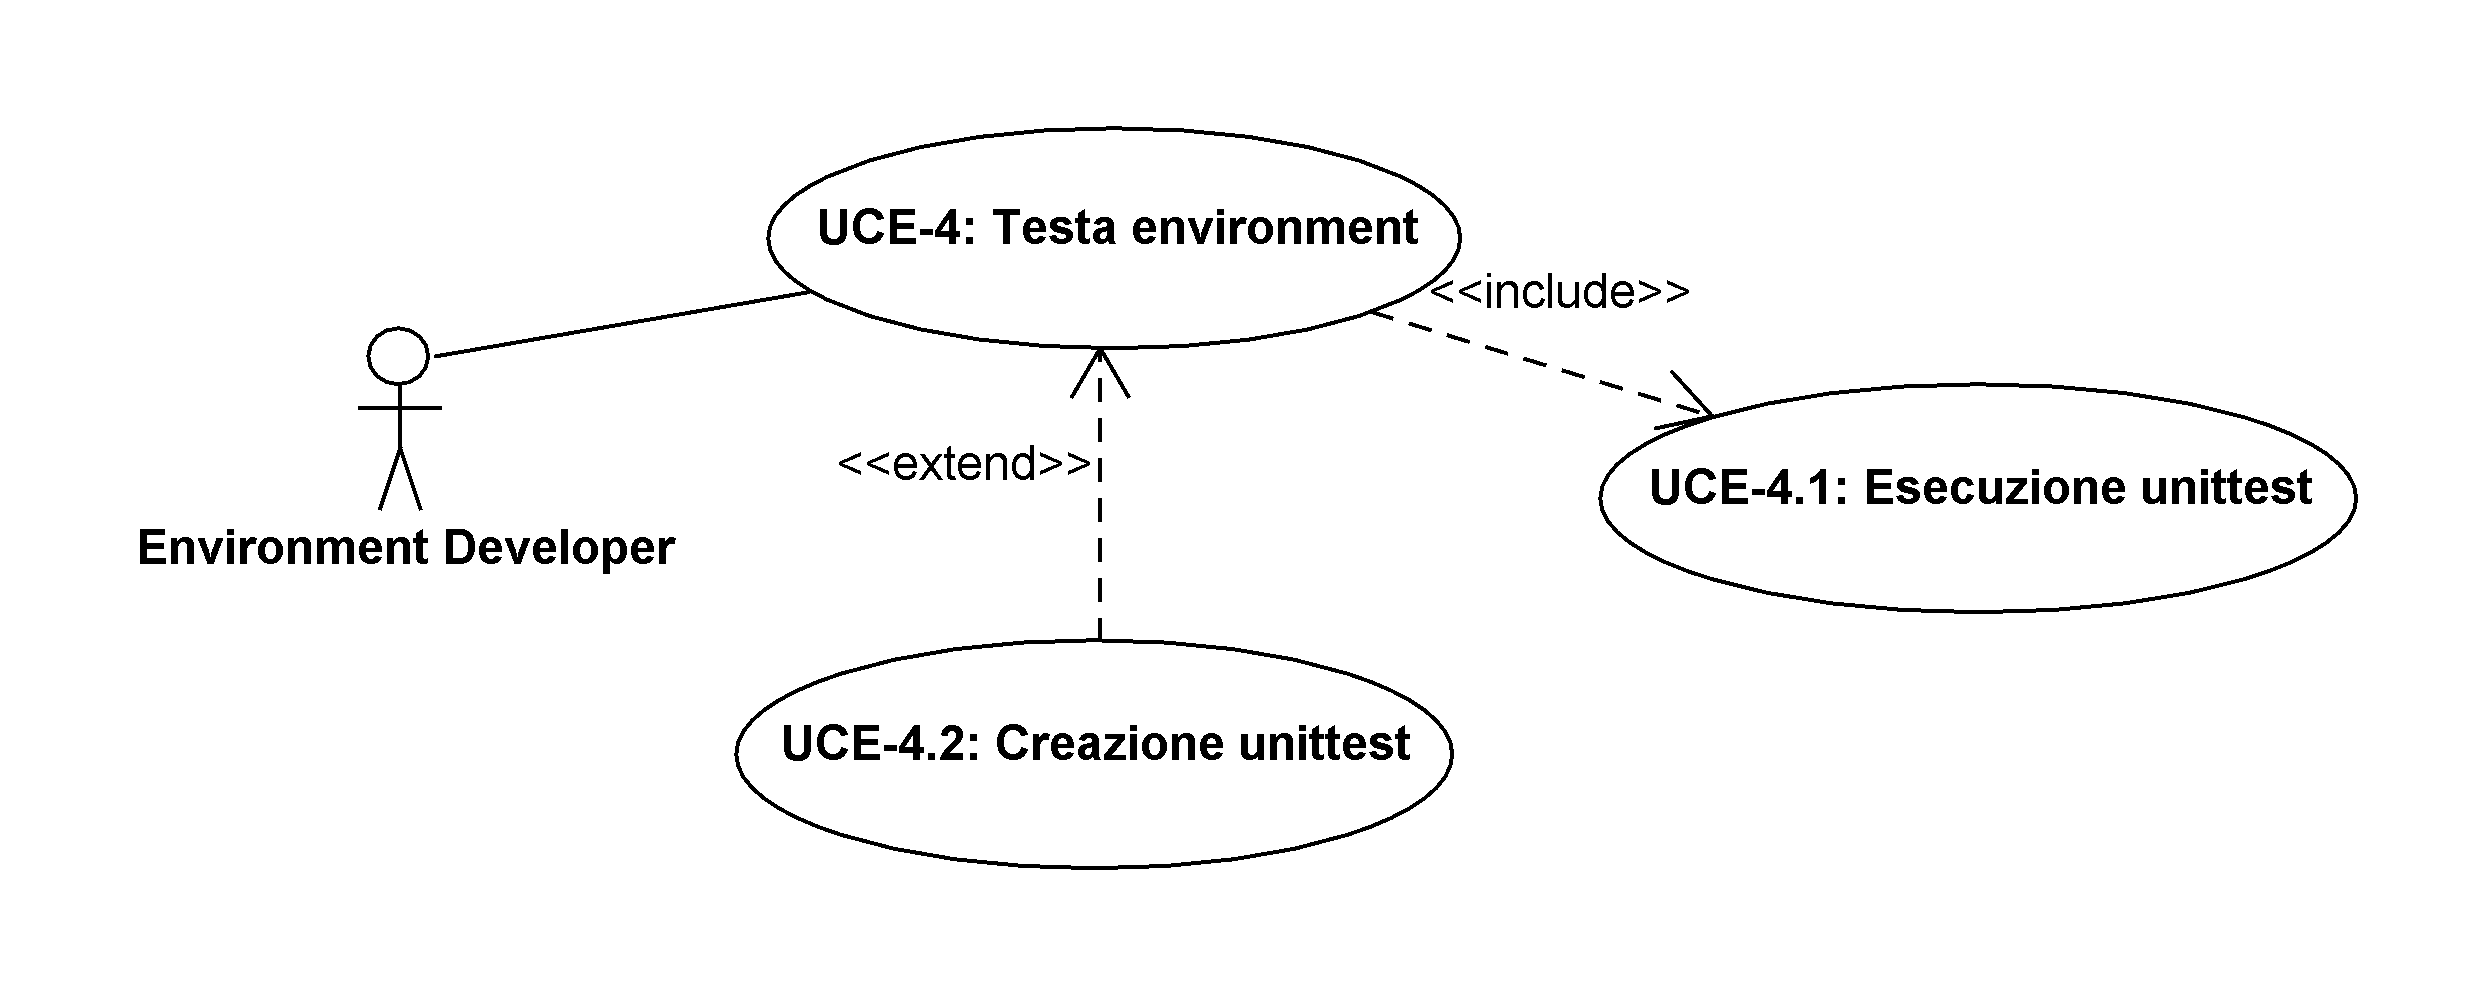
\includegraphics[width=1.1\textwidth]{Immagini/Capitolo2/UseCases/UCE-4.png}
\caption{Diagramma dei casi d'uso UCE-4}\label{fig:uc-uce-4}
\end{figure}

La descrizione comprende quella del caso d'uso \emph{UCE-4.1}.

\begin{itemize}
	\item \textbf{Attori:} ED
	\item \textbf{Scopo e descrizione:} l'ED deve essere in grado di verificare il funzionamento dell'environment utilizzando dei test d'unità. L'ED deve avere la possibilità di realizzare dei test d'unità per le funzionalità aggiunte
	\item \textbf{Pre-condizioni:} il software fornisce meccanismi per l'esecuzione di test d'unità in grado di verificare il comportamento dei componenti di sistema. Il software fornisce un framework per la definizione di nuovi test d'unità per le funzionalità introdotte
	\item \textbf{Post-condizioni:} l'ED ottiene dal software un riepilogo sul funzionamento delle componenti
	\item \textbf{Flusso principale degli eventi:}
		\begin{enumerate}
			\item l'ED avvia l'esecuzione dei test d'unità (\emph{UCE-4.1})
			\item l'ED ottiene un riepilogo dei risultati dei test
				\begin{itemize}
					\item il riepilogo indica eventuali test falliti
					\item il riepilogo indica il motivo del fallimento dei test
				\end{itemize}
		\end{enumerate}
\end{itemize}


\paragraph{UCE-4.1: Creazione unittest}

\begin{itemize}
	\item \textbf{Attori:} ED
	\item \textbf{Scopo e descrizione:} l'ED deve avere la possibilità di definire ed eseguire test d'unità in grado di verificare il corretto funzionamento delle caratteristiche aggiunte
	\item \textbf{Pre-condizioni:} il sistema è stato configurato correttamente. Il software offre meccanismi per l'integrazione di nuovi test d'unità a quelli forniti con il sistema
	\item \textbf{Post-condizioni:} un nuovo test d'unità è integrato con quelli forniti dal sistema
	\item \textbf{Flusso principale degli eventi:}
		\begin{enumerate}
			\item l'ED realizza un nuovo test d'unità
			\item l'ED registra il nuovo test d'unità insieme a quelli forniti dal software
		\end{enumerate}
\end{itemize}

\pagebreak

\subsubsection{UCA-1: Avvia Server}

%UCA-1: Avvia server

\begin{itemize}
	\item \textbf{Attori:} Server Administrator
	\item \textbf{Scopo e descrizione:} il Server Administrator deve essere in inizializzare un'istanza server del software
	\item \textbf{Pre-condizioni:} il sistema è correttamente configurato. Il software è correttamente configurato
	\item \textbf{Post-condizioni:} un'istanza server del software è attiva e attende connessioni
	\item \textbf{Flusso principale degli eventi:}
		\begin{enumerate}
			\item il Server Administrator avvia un'istanza del software
			\item la configurazione del software viene valutata (si guardi caso d'uso \emph{UCA-3})
		\end{enumerate}
	\item \textbf{Flusso alternativo \#1:}
		\begin{enumerate}
			\setcounter{enumi}{1}
			\item se una specifica di configurazione non è disponibile, il software notifica l'errore
			\item vengono utilizzati dei parametri di default
		\end{enumerate}
	\item \textbf{Flusso alternativo \#2:}
		\begin{enumerate}
			\setcounter{enumi}{1}
			\item se la specifica di configurazione non è valida, il software notifica l'errore
			\item l'esecuzione viene terminata
		\end{enumerate}
\end{itemize}
\pagebreak

\subsubsection{UCA-2: Arresta Server}

%UCA-2: Arresta Server

\begin{itemize}
	\item \textbf{Attori:} Server Administrator
	\item \textbf{Scopo e descrizione:} il Server Administrator deve essere in terminare l'esecuzione di un'istanza del software
	\item \textbf{Pre-condizioni:} un'istanza del software è attiva
	\item \textbf{Post-condizioni:} l'istanza del software non è più attiva
	\item \textbf{Flusso principale degli eventi:}
		\begin{enumerate}
			\item il Server Administrator richiede l'arresto del software
			\item tutte le sessioni vengono chiuse
			\item il software viene arrestato
		\end{enumerate}
	\item \textbf{Flusso alternativo:}
		\begin{enumerate}
			\setcounter{enumi}{1}
			\item se si verifica un errore durante la chiusura di una sessione (o un tempo limite per l'operazione viene superato), la sessione viene distrutta forzatamente
			\item lo scenario prosegue dal punto 3 del flusso principale
		\end{enumerate}
\end{itemize}
\pagebreak

\subsubsection{UCA-3: Configura Server}

%UCA-3: Configura Server

\begin{figure}
\centering
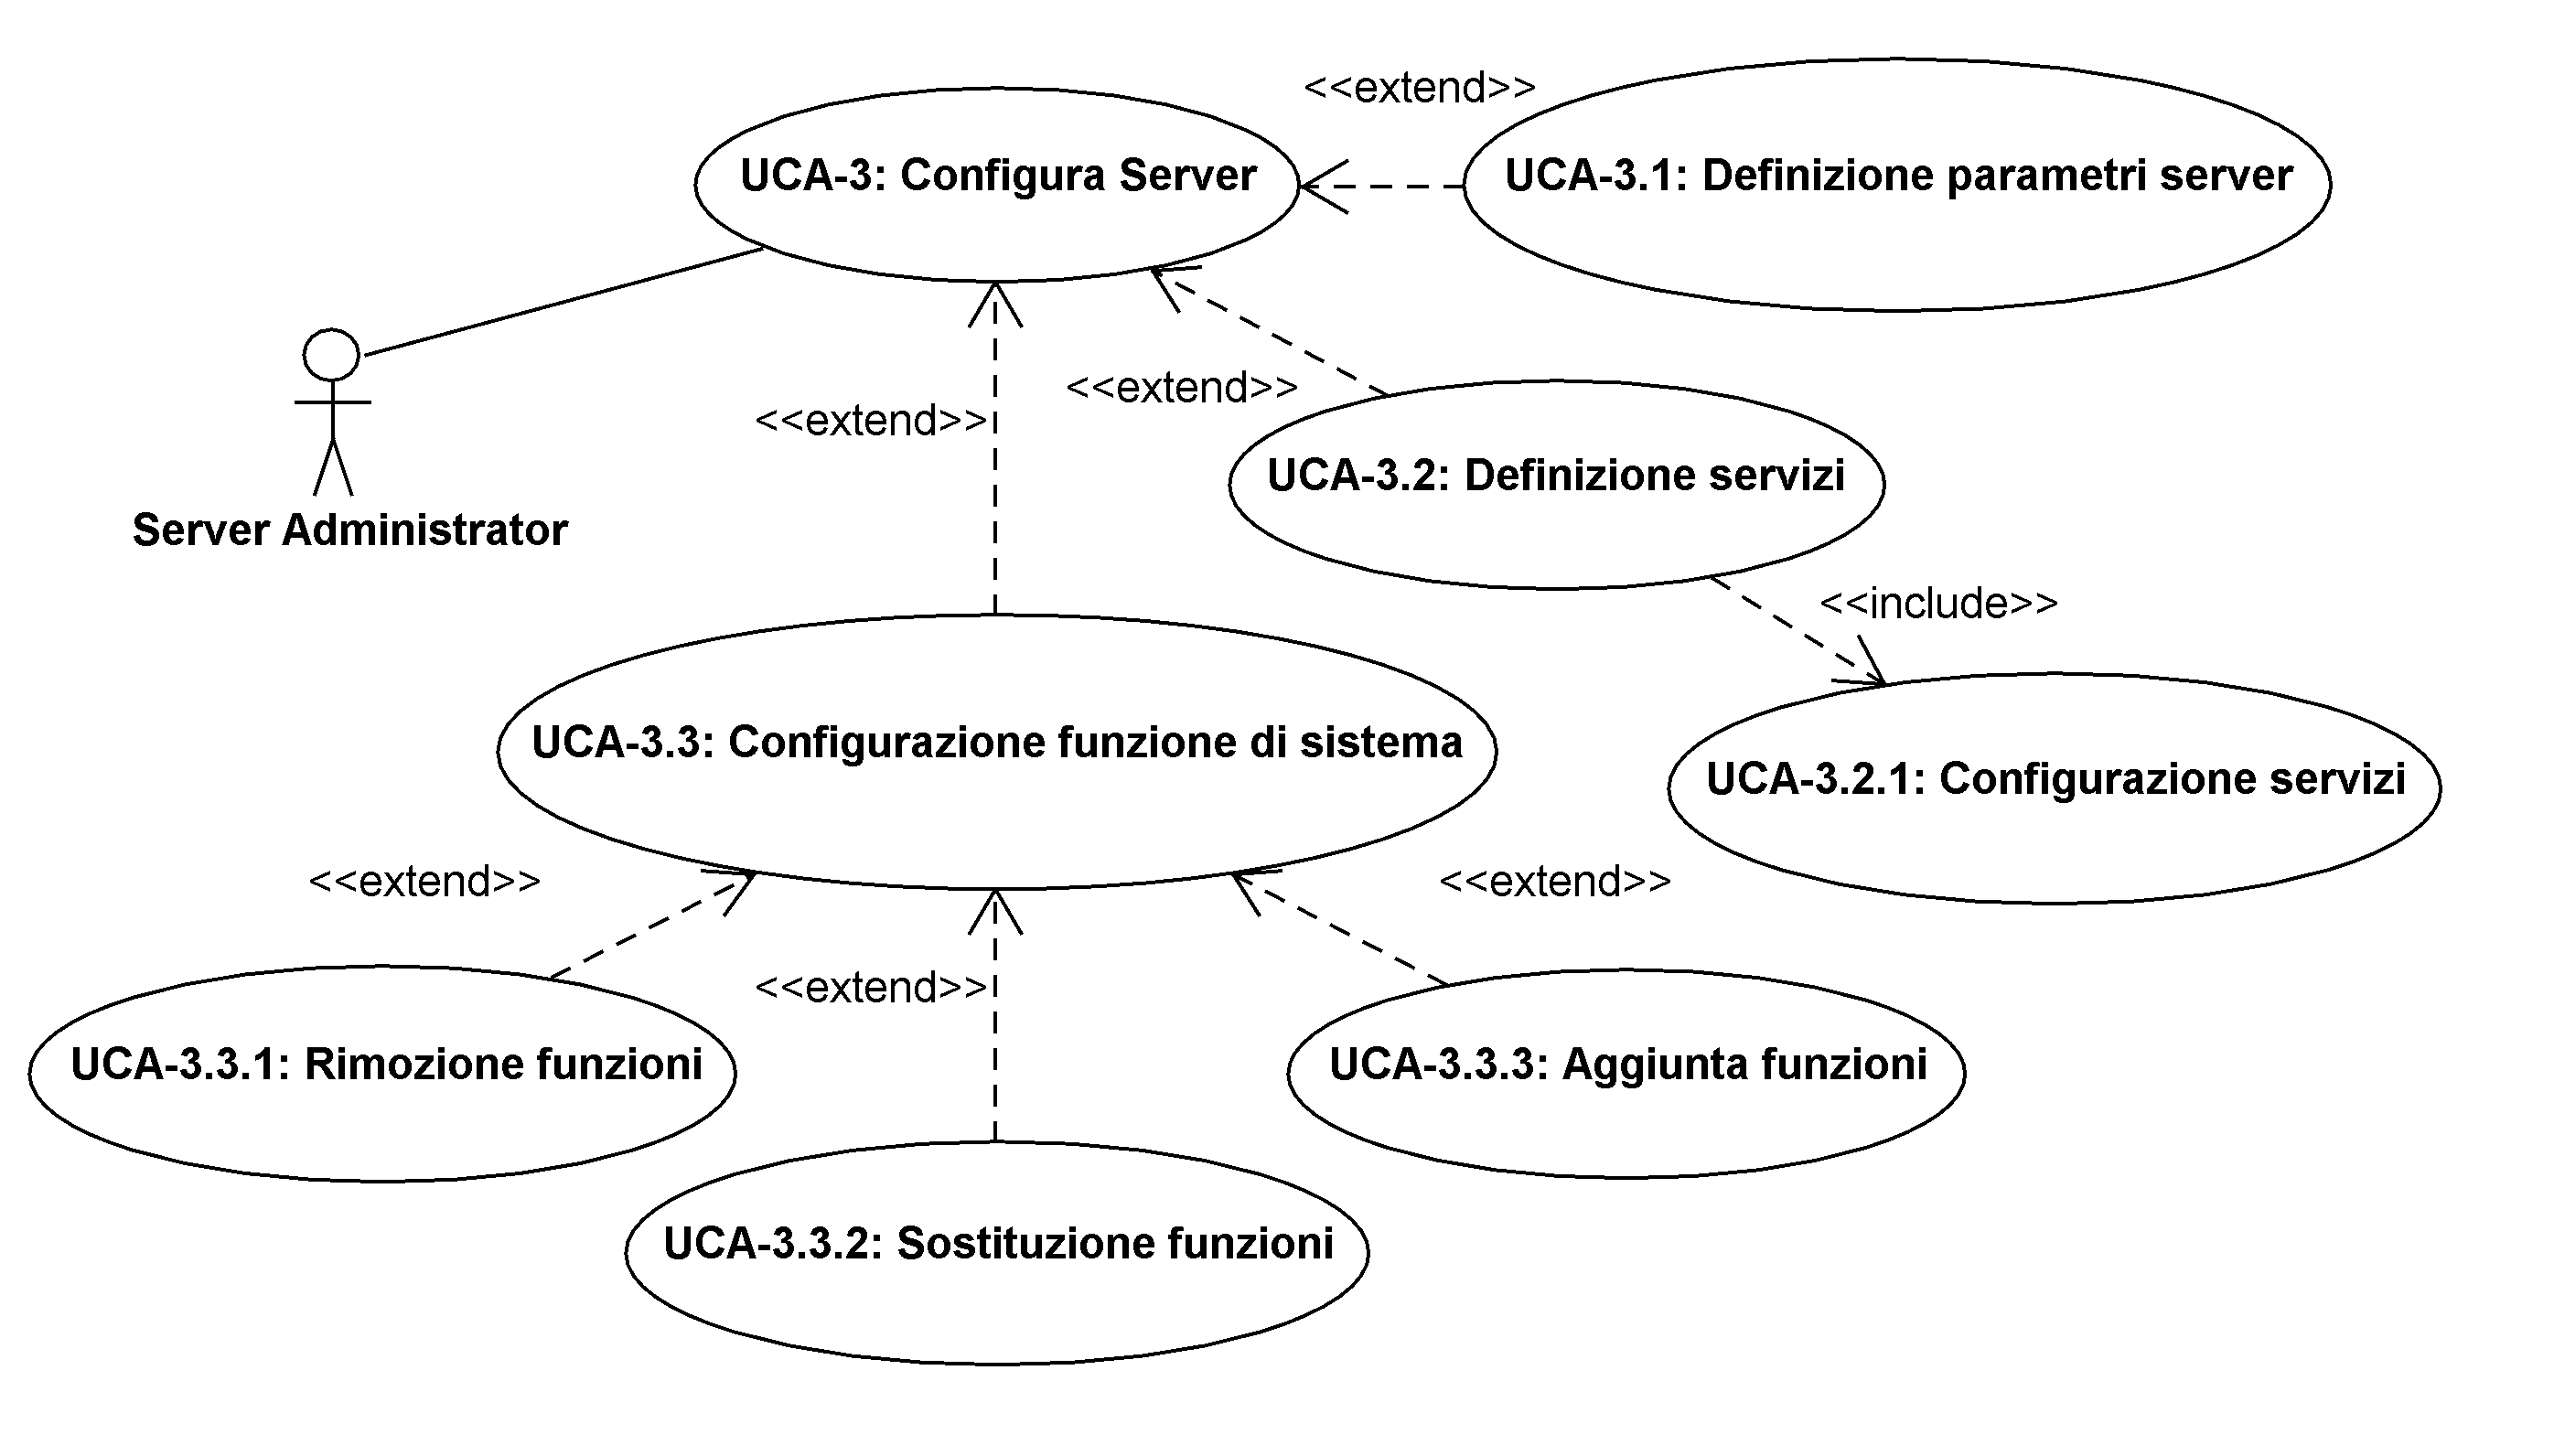
\includegraphics[width=1.1\textwidth]{Immagini/Capitolo2/UseCases/UCA-3.png}
\caption{Diagramma dei casi d'uso UCA-3}\label{fig:uc-uca-3}
\end{figure}

\begin{itemize}
	\item \textbf{Attori:} Server Administrator
	\item \textbf{Scopo e descrizione:} il Server Administrator deve avere la possibilità di configurare le funzioni del software MyCLIPS utilizzabili dai client, i servizi offerti dal server e i parametri di base del modulo server attraverso un file di configurazione
	\item \textbf{Pre-condizioni:} il sistema offre un formato di specifica delle configurazioni e un meccanismo di caricamento delle stesse
	\item \textbf{Post-condizioni:} il funzionamento del software rispecchia i parametri definiti del file di configurazione
	\item \textbf{Flusso principale degli eventi:}
		\begin{enumerate}
			\item il Server Administrator apre il file di configurazione attraverso un programma di \emph{text-editing}
			\item il Server Administrator modifica i parametri di configurazione del server
				\begin{itemize}
					\item il Server Administrator modifica le funzioni di MyCLIPS utilizzabili dai client (si guardi il caso d'uso \emph{UCA-3.3})
					\item il Server Administrator modifica i servizi attivi offerti dal server (si guardi il caso d'uso \emph{UCA-3.2})
					\item il Server Administrator modifica i parametri di base del server (si guardi il caso d'uso \emph{UCA-3.1})
				\end{itemize}
			\item il Server Administrator salva le modifiche
		\end{enumerate}
\end{itemize}


\paragraph{UCA-3.1: Configurazione parametri server}

\begin{itemize}
	\item \textbf{Attori:} Server Administrator
	\item \textbf{Scopo e descrizione:} il Server Administrator deve avere la possibilità di modificare i parametri di configurazione di base del server
	\item \textbf{Pre-condizioni:} \emph{nessuna}
	\item \textbf{Post-condizioni:} i parametri di configurazione risultano modificati secondo le aspettative del Server Administrator
	\item \textbf{Flusso principale degli eventi:}
		\begin{enumerate}
			\item il Server Administrator modifica i parametri di base del server. Può configurare:
				\begin{itemize}
					\item l'indirizzo di ascolto (\emph{bind-address})
					\item la porta di ascolto (\emph{bind-port})
					\item la creazione di un registro delle richieste (\emph{log-requests})
					\item il livello di dettaglio del registro delle richieste (\emph{log-level})
				\end{itemize}
		\end{enumerate}
\end{itemize}


\paragraph{UCA-3.2: Definizione servizi}

La descrizione comprende anche quella del caso d'uso \emph{UCA-3.2.1}.

\begin{itemize}
	\item \textbf{Attori:} Server Administrator
	\item \textbf{Scopo e descrizione:} il Server Administrator deve avere la possibilità di definire i servizi attivi offerti dal server e configurare i parametri di funzionamento dei servizi
	\item \textbf{Pre-condizioni:} \emph{nessuna}
	\item \textbf{Post-condizioni:} i parametri di configurazione risultano modificati secondo le aspettative del Server Administrator
	\item \textbf{Flusso principale degli eventi:}
		\begin{enumerate}
			\item il Server Administrator modifica i servizi attivi offerti dal server specificando:
				\begin{itemize}
					\item l'interfaccia offerta dal servizio
					\item un'implementazione del servizio
				\end{itemize}
			\item il Server Administrator specifica i parametri relativi ai servizi attivi (\emph{UCA-3.2.1)}: il formato, il tipo e i valori delle configurazioni sono definite dalla specifica implementazione del servizio
		\end{enumerate}
\end{itemize}





\pagebreak

\subsubsection{UCS-1: Analisi dei risultati}

%UCS-1: Analisi dei risultati

\begin{figure}
\centering
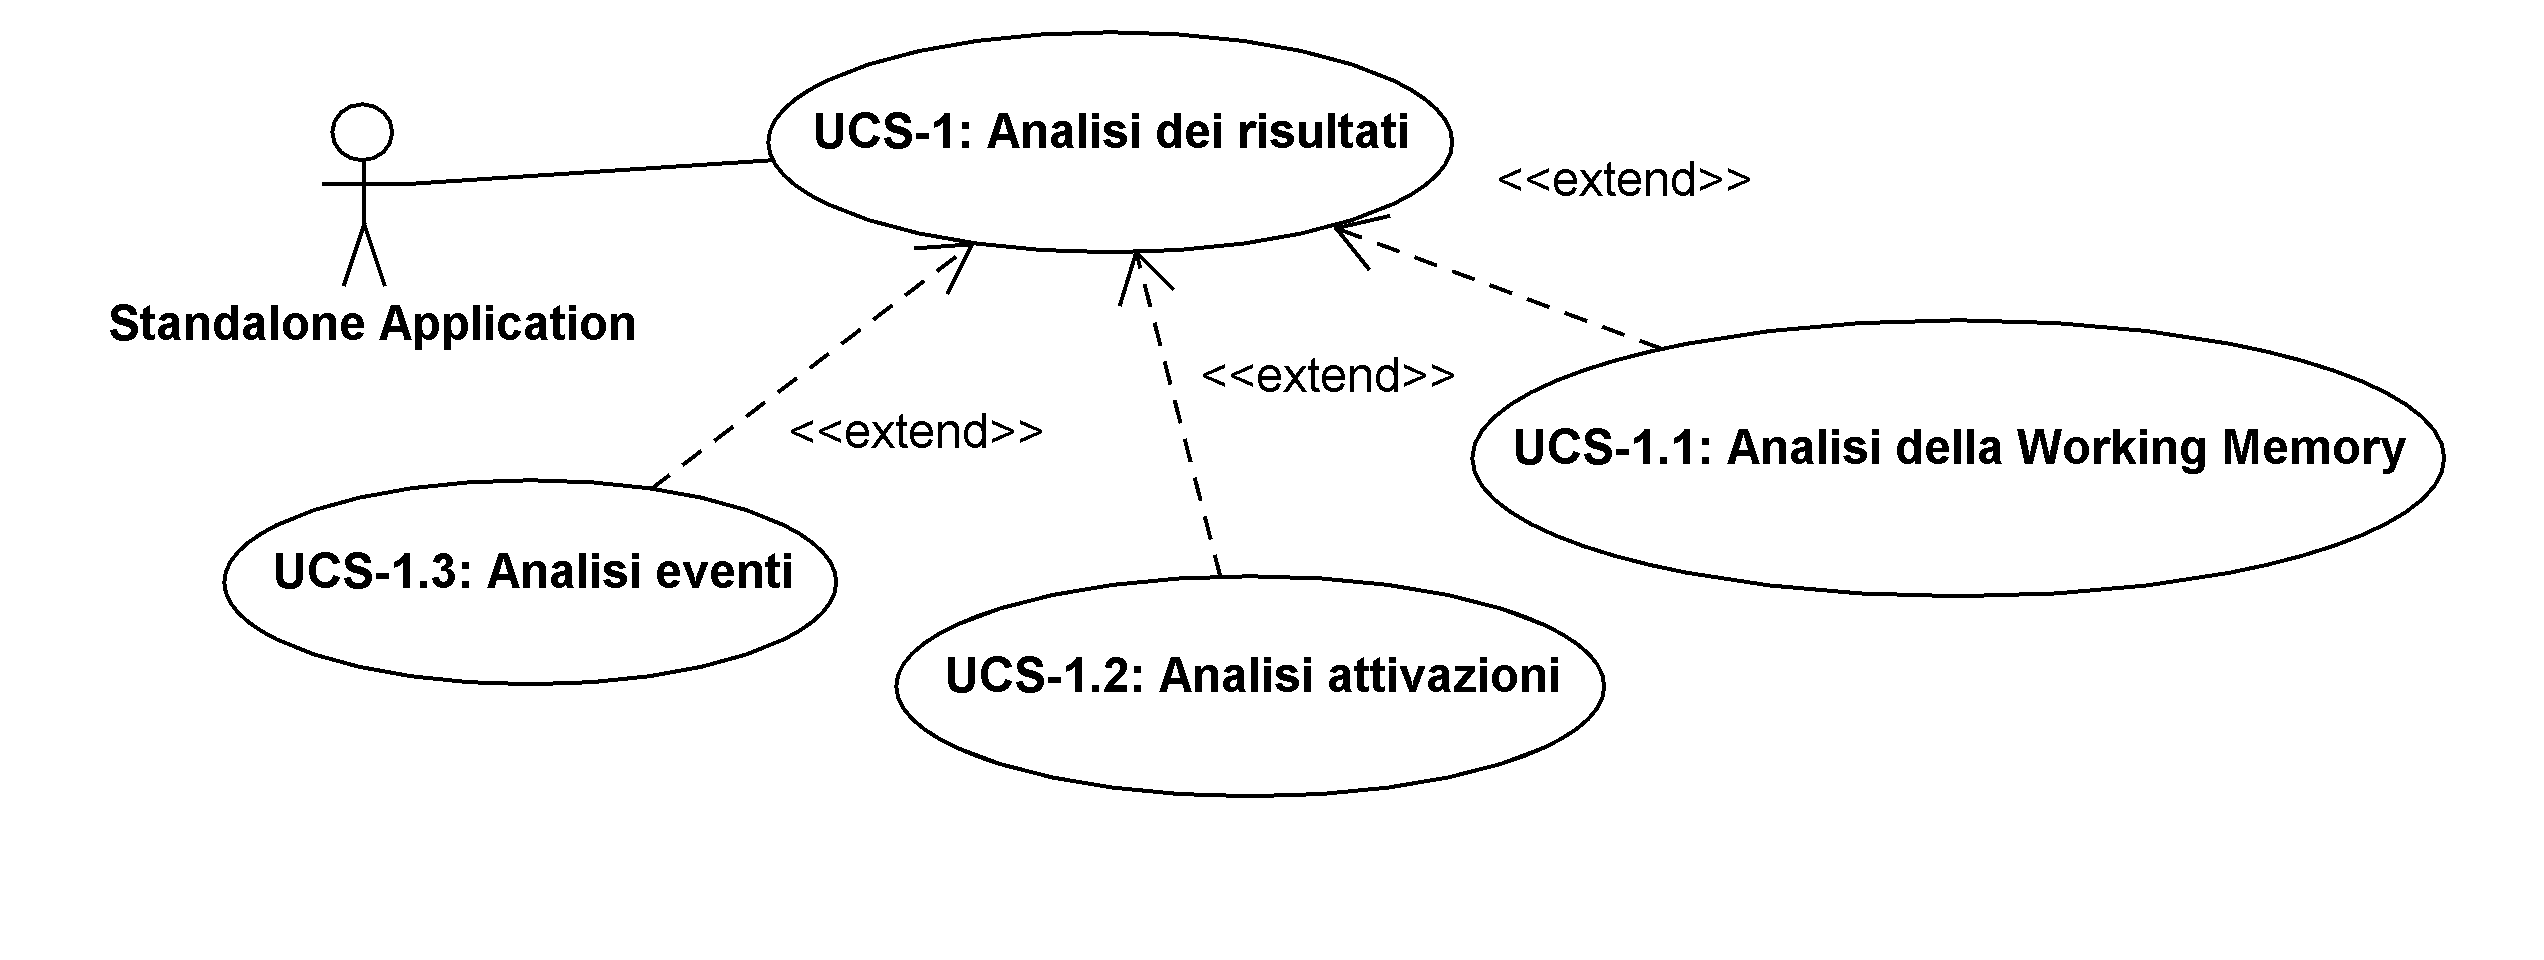
\includegraphics[width=1.1\textwidth]{Immagini/Capitolo2/UseCases/UCS-1.png}
\caption{Diagramma dei casi d'uso UCS-1}\label{fig:uc-ucs-1}
\end{figure}

\begin{itemize}
	\item \textbf{Attori:} Standalone Application
	\item \textbf{Scopo e descrizione:} la Standalone Application deve avere la possibilità di accedere alle informazioni riguardanti lo stato finale di un'elaborazione eseguita dal software e ricevere notifica del verificarsi di eventi durante l'elaborazione
	\item \textbf{Pre-condizioni:} la Standalone Application ha eseguito con successo il caso d'uso \emph{UCC-1.2}
	\item \textbf{Post-condizioni:} la Standalone Application ha ottenuto le informazioni necessarie
	\item \textbf{Flusso principale degli eventi:}
		\begin{enumerate}
			\item la Standalone Application richiede informazioni sullo stato terminale di elaborazione del software
				\begin{itemize}
					\item la Standalone Application richiede informazioni sullo stato della \emph{working-memory} (si guardi il caso d'uso \emph{UCS-1.1})
					\item la Standalone Application richiede informazioni sullo stato delle attivazioni ancora presenti (si guardi il caso d'uso \emph{UCS-1.2})
					\item la Standalone Application valuta il verificarsi di un evento (si guardi il caso d'uso \emph{UCS-1.3})
				\end{itemize}
			\item la Standalone Application ottiene le informazioni richieste
		\end{enumerate}
\end{itemize}


\paragraph{UCS-1.1: Analisi della Working-Memory}

\begin{itemize}
	\item \textbf{Attori:} Standalone Application
	\item \textbf{Scopo e descrizione:} la Standalone Application deve avere accesso alle informazioni presenti nella \emph{Working Memory}
	\item \textbf{Pre-condizioni:} la Standalone Application ha eseguito con successo il caso d'uso \emph{UCC-1.2}
	\item \textbf{Post-condizioni:} la Standalone Application ottiene le informazioni sui fatti presenti nella \emph{Working Memory}
	\item \textbf{Flusso principale degli eventi:}
		\begin{enumerate}
			\item la Standalone Application richiede una vista dei dati presenti nella \emph{Working Memory}
				\begin{itemize}
					\item la Standalone Application può limitare la ricerca solo ai fatti relativi ad un sottogruppo dei moduli specificati
					\item la Standalone Application può richiedere tutti i fatti presenti nella \emph{Working Memory}
				\end{itemize}
			\item la Standalone Application ottiene l'elenco dei fatti richiesti
		\end{enumerate}
\end{itemize}


\paragraph{UCS-1.2: Analisi attivazioni}

\begin{itemize}
	\item \textbf{Attori:} Standalone Application
	\item \textbf{Scopo e descrizione:} la Standalone Application deve avere accesso alle informazioni presenti nell'agenda delle attivazioni
	\item \textbf{Pre-condizioni:} la Standalone Application ha eseguito con successo il caso d'uso \emph{UCC-1.1}
	\item \textbf{Post-condizioni:} la Standalone Application ottiene l'elenco di attivazioni disponibili nell'agenda delle attivazioni nelle modalità che ha indicato
	\item \textbf{Flusso principale degli eventi:}
		\begin{enumerate}
			\item la Standalone Application richiede una vista sulle attivazioni presenti nell'agenda delle attivazioni.
				\begin{itemize}
					\item la Standalone Application può limitare la ricerca solo alle attivazioni relative ad un sottogruppo dei moduli specificati
					\item la Standalone Application può richiedere l'intera lista delle attivazioni presenti in agenda
				\end{itemize}
			\item la Standalone Application ottiene l'elenco delle attivazioni richieste
		\end{enumerate}
\end{itemize}


\paragraph{UCS-1.3: Analisi eventi}

\begin{itemize}
	\item \textbf{Attori:} Standalone Application
	\item \textbf{Scopo e descrizione:} la Standalone Application deve ricevere notifica del verificarsi di un evento per il quale ha espresso interesse nelle modalità previste dal software
	\item \textbf{Pre-condizioni:} la Standalone Application ha eseguito con successo il caso d'uso \emph{UCC-1.2.3}
	\item \textbf{Post-condizioni:} la Standalone Application ha eseguito il comportamento associato ad un determinato evento
	\item \textbf{Flusso principale degli eventi:}
		\begin{enumerate}
			\item la Standalone Application esprime interesse relativamente al verificarsi di un evento (si guardi caso d'uso \emph{UCC-1.2.3})
			\item la Standalone Application osserva la notifica del verificarsi di un evento
			\item la Standalone Application analizza i parametri relativi all'evento
			\item la Standalone Application esegue il comportamento associato all'evento con i parametri forniti
		\end{enumerate}
\end{itemize}





\pagebreak

\subsubsection{UCR-1: Inizializza sessione}

%UCR-1: Inizializza sessione

\begin{figure}
\centering
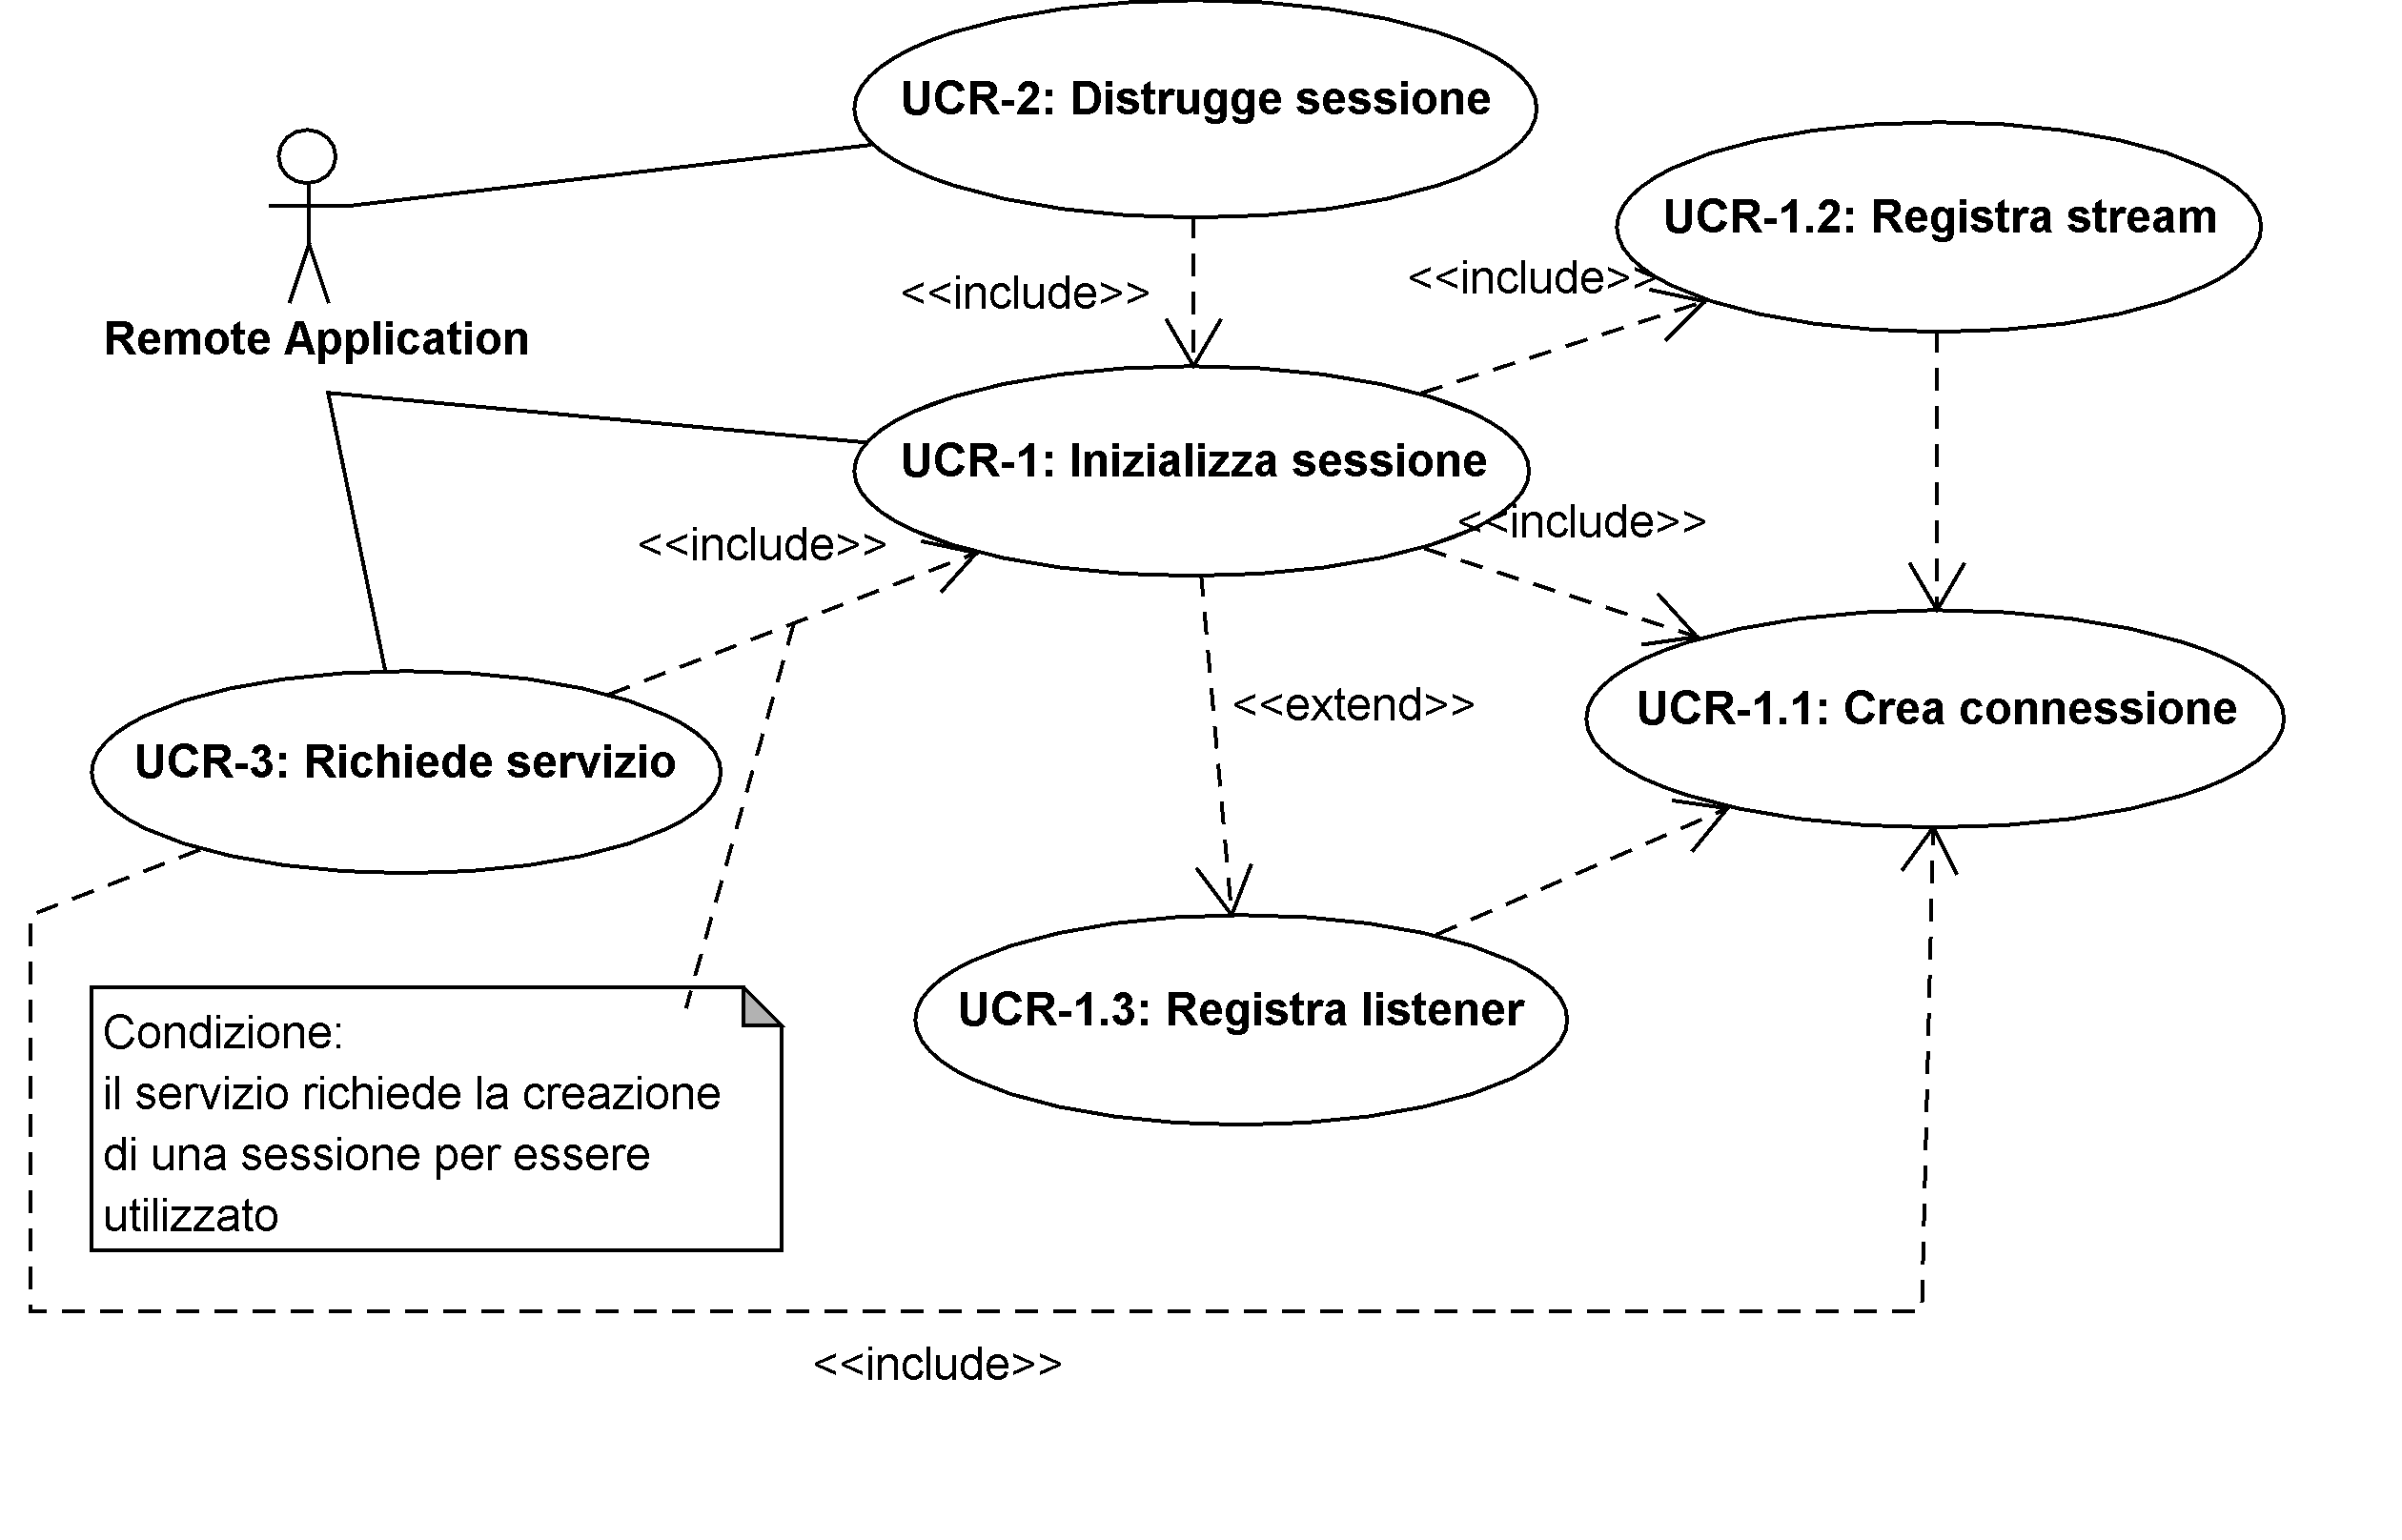
\includegraphics[width=1.1\textwidth]{Immagini/Capitolo2/UseCases/UCR-generale.png}
\caption{Diagramma dei casi d'uso UCR-1, UCR-2, UCR-3}\label{fig:uc-ucr-generale}
\end{figure}

Nel proseguo dei paragrafi relativi ai casi d'uso \emph{UCR}, il nome dell'attore \emph{Remote Application} verrà abbreviato con la sigla \emph{RA}.

\begin{itemize}
	\item \textbf{Attori:} Remote Application (\emph{RA})
	\item \textbf{Scopo e descrizione:} la RA deve avere la possibilità di inizializzare una sessione persistente con il software server che memorizzi le informazioni i dati che devono essere conservati fra richieste differenti
	\item \textbf{Pre-condizioni:} la RA ha conoscenza dei parametri di connessione relativi ad una istanza del software server
	\item \textbf{Post-condizioni:} la RA ottiene un codice univoco che identifica la sessione creata
	\item \textbf{Flusso principale degli eventi:}
		\begin{enumerate}
			\item la RA esegue una connessione con il server (si guardi il caso d'uso \emph{UCR-1.1})
			\item la RA richiede l'inizializzazione di una sessione
				\begin{itemize}
					\item la RA può fornire al server i parametri di connessione di uno stream (si guardi il caso d'uso \emph{UCR-1.2})
					\item la RA può fornire al server i parametri di connessione di un listener (si guardi il caso d'uso \emph{UCR-1.3})
				\end{itemize}
			\item la RA memorizza l'identificativo di sessione
		\end{enumerate}
	\item \textbf{Flusso alternativo:}
		\begin{enumerate}
			\setcounter{enumi}{1}
			\item se la RA non ottiene l'identificativo di sessione, lo scenario prosegue dal punto 1 del flusso principale
		\end{enumerate}
\end{itemize}


\paragraph{UCR-1.1: Crea connessione}

\begin{itemize}
	\item \textbf{Attori:} RA
	\item \textbf{Scopo e descrizione:} la RA deve avere la possibilità di stabilire una connessione con il server tramite protocollo XML-RPC
	\item \textbf{Pre-condizioni:} la RA ha conoscenza dei parametri di connessione relativi ad una istanza del software server
	\item \textbf{Post-condizioni:} la RA ha stabilito una connessione. Permette l'esecuzione dei casi d'uso \emph{UCR-1}, \emph{UCR-1.2}, \emph{UCR-1.3}, \emph{UCR-3}
	\item \textbf{Flusso principale degli eventi:}
		\begin{enumerate}
			\item la RA stabilisce una connessione seguendo le specifiche del protocollo XML-RPC
		\end{enumerate}
	\item \textbf{Flusso alternativo:}
		\begin{enumerate}
			\item se la connessione fallisce, la RA attiva un protocollo di gestione dell'errore (la definizione del protocollo è materia della RA)
		\end{enumerate}
\end{itemize}


\paragraph{UCR-1.2: Registra stream}

\begin{itemize}
	\item \textbf{Attori:} RA
	\item \textbf{Scopo e descrizione:} la RA deve essere in grado di registrare uno stream remoto utilizzabile dal software server 
	\item \textbf{Pre-condizioni:} la RA ha eseguito con successo il caso d'uso \emph{UCR-1.1}
	\item \textbf{Post-condizioni:} il software server può utilizzare lo stream remoto come sostituto di uno locale. Permette l'esecuzione dei casi d'uso \emph{UCC-1.2.1} e \emph{UCC-1.2.2} anche per l'attore RA
	\item \textbf{Flusso principale degli eventi:}
		\begin{enumerate}
			\item la RA fornisce al software server i parametri di connessione di uno stream remoto
			\item la RA indica:
				\begin{enumerate}
					\item indirizzo e porta di connessione dello stream
					\item nome dello stream remoto
					\item nome dello stream per il software server
					\item un codice di controllo
				\end{enumerate}
			\item la RA riceve un segnale di conferma all'indirizzo indicato usando i parametri forniti
			\item lo stream remoto è indicato come sostituto di uno stream locale
		\end{enumerate}
	\item \textbf{Flusso alternativo:}
		\begin{enumerate}
			\setcounter{enumi}{2}
			\item se la RA non ottiene un segnale di conferma dopo un tempo massimo stabilito, la RA attiva un protocollo di gestione dell'errore (la definizione del protocollo è materia della RA)
			\item lo stream remoto viene ignorato
		\end{enumerate}
\end{itemize}


\paragraph{UCR-1.3: Registra listener}

\begin{itemize}
	\item \textbf{Attori:} RA
	\item \textbf{Scopo e descrizione:} la RA deve essere in grado di registrare un listener remoto utilizzabile dal software server 
	\item \textbf{Pre-condizioni:} la RA ha eseguito con successo il caso d'uso \emph{UCR-1.1}
	\item \textbf{Post-condizioni:} il software server può utilizzare il listener remoto come sostituto di uno locale. Permette l'esecuzione del caso d'uso \emph{UCC-1.2.3} anche per l'attore RA
	\item \textbf{Flusso principale degli eventi:}
		\begin{enumerate}
			\item la RA fornisce al software server i parametri di connessione di un listener remoto
			\item la RA indica:
				\begin{enumerate}
					\item indirizzo e porta di connessione del listener
					\item nome del listener remoto
					\item nome del listener per il software server
					\item il nome degli eventi per i quali registrare il listener
					\item un codice di controllo
				\end{enumerate}
			\item la RA riceve un segnale di conferma all'indirizzo indicato usando i parametri forniti
			\item il listener remoto è indicato come sostituto di uno locale
		\end{enumerate}
	\item \textbf{Flusso alternativo:}
		\begin{enumerate}
			\setcounter{enumi}{2}
			\item se la RA non ottiene un segnale di conferma dopo un tempo massimo stabilito, la RA attiva un protocollo di gestione dell'errore (la definizione del protocollo è materia della RA)
			\item il listener remoto viene ignorato
		\end{enumerate}
\end{itemize}



\pagebreak

\subsubsection{UCR-2: Distrugge sessione}

%UCR-2: Distrugge sessione

Il diagramma relativo al caso d'uso \emph{UCR-2}, data la natura complessa dello stesso, è accorpato a quello del caso d'uso \emph{UCR-1} fornito in \figurename~\ref{fig:uc-ucr-generale}.

\begin{itemize}
	\item \textbf{Attori:} RA
	\item \textbf{Scopo e descrizione:} la RA deve avere la possibilità di terminare e distruggere una sessione precedentemente inizializzata
	\item \textbf{Pre-condizioni:} la RA ha eseguito il caso d'uso \emph{UCR-1}
	\item \textbf{Post-condizioni:} il codice univoco ottenuto dall'esecuzione del caso d'uso \emph{UCR-1} non è più valido
	\item \textbf{Flusso principale degli eventi:}
		\begin{enumerate}
			\item la RA notifica la volontà di terminare la sessione al software server
			\item la RA riceve notifica di avvenuta chiusura della sessione
			\item la RA cancella dalla propria memoria il codice univoco di sessione
		\end{enumerate}
	\item \textbf{Flusso alternativo:}
		\begin{enumerate}
			\setcounter{enumi}{1}
			\item se la RA non riceve notifica di avvenuta chiusura della sessione dopo un tempo stabilito, notifica un avviso non invasivo
			\item lo scenario prosegue dal punto 3 del flusso principale
		\end{enumerate}
\end{itemize}
\pagebreak

\subsubsection{UCR-3: Richiede servizio}

%UCR-3: Richiede servizio

Il diagramma relativo al caso d'uso \emph{UCR-3}, data la natura complessa dello stesso, è accorpato a quello del caso d'uso \emph{UCR-1} fornito in \figurename~\ref{fig:uc-ucr-generale}.

\begin{itemize}
	\item \textbf{Attori:} RA
	\item \textbf{Scopo e descrizione:} la RA deve avere la possibilità di richiedere un servizio al software server
	\item \textbf{Pre-condizioni:} la RA ha eseguito il caso d'uso \emph{UCR-1.1}. La RA ha eseguito il caso d'uso \emph{UCR-1} se il servizio richiesto richiede l'inizializzazione di una sessione
	\item \textbf{Post-condizioni:} la RA ha ottenuto il risultato dell'elaborazione effettuata da un servizio
	\item \textbf{Flusso principale degli eventi:}
		\begin{enumerate}
			\item la RA richiede un servizio al software server
				\begin{itemize}
					\item la RA indica il nome del servizio richiesto
					\item la RA indica i parametri di esecuzione del servizio
					\item la RA può indicare il codice univoco di una sessione precedentemente inizializzata, se necessario
				\end{itemize}
			\item la RA attende il completamento dell'elaborazione
		\end{enumerate}
	\item \textbf{Flusso alternativo \#1:}
		\begin{enumerate}
			\item se la RA richiede un servizio non disponibile, la RA riceve un messaggio d'errore
			\item la RA attiva un protocollo di gestione dell'errore (la definizione del protocollo è materia della RA)
		\end{enumerate}

	\item \textbf{Flusso alternativo \#2:}
		\begin{enumerate}
			\item se la RA richiede un servizio disponibile, ma il codice di sessione è scaduto
			\item la RA esegue il caso d'uso \emph{UCR-1}
			\item lo scenario prosegue dal punto 1 del flusso principale
		\end{enumerate}

		
	\item \textbf{Flusso alternativo \#3:}
		\begin{enumerate}
			\setcounter{enumi}{1}
			\item se la RA non riceve risposta entro un tempo limite, la RA attiva un protocollo di gestione dell'errore (la definizione del protocollo è materia della RA)
		\end{enumerate}
\end{itemize}
\pagebreak


%\section{Requisiti}

%\subsection{Generale}

